\documentclass[a4paper,12pt]{report}

\usepackage{alltt, fancyvrb, url}
\usepackage{graphicx}
\usepackage[utf8]{inputenc}
\usepackage{float}
\usepackage{hyperref}
\usepackage{tikz}

% Questo commentalo se vuoi scrivere in inglese.
\usepackage[italian]{babel}

\usepackage[italian]{cleveref}

\title{Progetto di Programmazione ad Oggetti\\``The Exiled''}

\author{Luca Casadei, Francesco Pazzaglia, Marco Magnani, Manuel Baldoni}
\date{\today}


\begin{document}

\maketitle

\tableofcontents

\chapter{Analisi}

\section{Requisiti}
L'applicazione è un gioco che presenta un personaggio controllato dal giocatore con la possibilità di muoversi nella mappa in 4 direzioni e di combattere contro dei nemici utilizzando magie elementali. I nemici sconfitti potrebbero rilasciare delle cure o dei potenziamenti che favoriscono il giocatore. Per concludere il gioco, il giocatore deve entrare in possesso di 4 cristalli che vengono consegnati una volta sconfitti i 4 boss del gioco che sono nemici più difficili da sconfiggere.
\subsection*{Requisiti funzionali}
\begin{itemize}
    \item Movimento del giocatore.
    \item Movimento dei nemici.
    \item Presenza di oggetti ottenibili dal giocatore (Cure, potenziamenti e cristalli).
    \item Terminazione del gioco una volta raccolti 4 cristalli o se il giocatore viene sconfitto.
    \item Rilascio degli oggetti da parte dei nemici.
    \item Possibilità di fare battaglie tra giocatore e nemici.
    \item Nemici più forti (boss) che se sconfitti rilasciano i cristalli per terminare il gioco.
    \item Possibilità di utilizzo di magie in battaglia di diverso tipo (Fuoco, Acqua, Fulmine, Erba).
    \item Aumento di livello tramite guadagno di esperienza sconfiggendo i nemici.
\end{itemize}

\subsection*{Requisiti non funzionali}
\begin{itemize}
    \item Il gioco deve essere multipiattaforma.
    \item L'interfaccia deve essere ridimensionabile.
\end{itemize}

\section{Analisi e modello del dominio}

\subsection{Inizio del gioco} \label{ss:iniziogioco}
All'inizio al giocatore viene chiesto di che tipo elementale sarà il personaggio da controllare (vedi \textit{\nameref{ss:tipi}}), quando verrà posizionato sulla mappa gli verrà assegnata una mossa generica di tipo normale, quelle invece del suo stesso tipo potranno essere imparate in maniera automatica all'aumentare di livello.\\

\subsection{Movimento}
Il giocatore può muoversi di una cella alla volta in una mappa a griglia in 4 direzioni (Nord, Est, Sud, Ovest), mentre si muove il giocatore, si muovono sempre di cella in cella anche i nemici, che non seguono un pattern di movimento specifico ma seguono una direzione casuale, questo a meno che non sia presente il giocatore nel loro range di visibilità (Configurabile da costante), in tal caso seguiranno il giocatore.\\ Il movimento del giocatore è libero su tutta la mappa, mentre i nemici sono costretti a stare nella zona del loro stesso tipo e non ne potranno uscire anche se in fase di inseguimento del player.\\

\subsection{Battaglia}
Una battaglia inizia se il giocatore e un nemico si ritrovano nella stessa cella a seguito di un movimento. Per affrontare un nemico in battaglia il giocatore ha a disposizione massimo 4 mosse (non per forza dello stesso tipo del giocatore). Il combattimento avviene a turni alternati, il primo è il giocatore, poi il nemico e così via finché uno dei due viene sconfitto, se è il giocatore, il gioco termina.\\
Allo sconfiggere dei nemici viene conferita al giocatore una certa quantità di esperienza (a seconda del nemico sconfitto) che serve ad aumentare di livello e vi è una certa probabilità che il nemico possa rilasciare un oggetto casuale (la probabilità maggiore è però quella di non ricevere nulla).

\subsection{Oggetti} \label{ss:oggetti}
Qualora venga rilasciato, l'oggetto verrà automaticamente messo nell'inventario del giocatore e potrà essere usato direttamente dalla mappa oppure in battaglia. Ci sono diversi tipi di oggetto, quelli utilizzabili dalla mappa generalmente sono oggetti di cura (rappresentati con il colore \colorbox{green}{verde}), altri possono essere oggetti che aumentano il danno del giocatore (colore \colorbox{red}{rosso}) oppure la difesa (colore \colorbox{cyan}{blu-azzurro}). Nessun nemico generico potrà rilasciare un \textit{Cristallo}, che è un oggetto esclusivo dei boss e serve per concludere il gioco.

\subsection{Livello ed esperienza}
L'aumento di livello comporta un incremento generale delle statistiche del giocatore, ovvero attacco, difesa e vita di un valore moltiplicativo o incrementale costante. Ogni $\mathit{n}$ livelli verrà presentata al giocatore la possibilità di imparare una nuova mossa, dove $\mathit{n}$ è una costante configurabile. se il giocatore ha già 4 mosse potrà decidere di scambiare quella nuova con una di quelle che conosce già. All'aumentare di livello sarà richiesta sempre più esperienza per passare a quello successivo.

\subsection{Nemici}
I nemici si dividono in nemici generici, ovvero quelli presenti sulla mappa con capacità di movimento, questi possono essere anche ripetuti e una volta sconfitti non ricompaiono. Ciascuno di questi ha un suo tipo elementale e quindi un'area della mappa a cui è confinato.
Per vedere i possibili oggetti rilasciati dai nemici, vedi \textit{\nameref{ss:oggetti}}.\\
I 4 boss sono posizionati agli angoli della mappa, e ciascuno di loro si trova nella parte di mappa che corrisponde al tipo elementale che rappresentano, i boss non hanno capacità di movimento e staranno in quella posizione finché non verranno sconfitti dal giocatore.

\subsection{Elenco dei tipi elementali} \label{ss:tipi}
I seguenti sono i tipi elementali presenti, ognuno è efficace rispetto ad un altro, quindi quando vengono usate mosse di un certo tipo risultante essere efficace rispetto al tipo di un nemico (non delle mosse che ha, proprio il tipo del nemico), si avranno dei moltiplicatori del danno. Lo stesso vale per i nemici che usano mosse di un tipo efficace rispetto a quello scelto dal giocatore all'inizio (la sua classe, vedi \textit{\nameref{ss:iniziogioco}}).
\\
Ad esempio, nel seguente schema si vede che Fulmine è efficace contro Acqua, Erba contro Fulmine etc\dots Se si capovolge la freccia si notano invece le debolezze di un tipo rispetto ad un altro.

\begin{center}
\begin{tabular}{ c c c }
    Fulmine & $\longrightarrow$ & Acqua \\
    Erba & $\longrightarrow$ & Fulmine \\
    Acqua & $\longrightarrow$ & Fuoco \\
    Fuoco & $\longrightarrow$ & Erba \\
\end{tabular}
\end{center}

\subsection{UML}
\begin{figure}[H]
	\centering
	% generated by Plantuml 1.2023.13      
\definecolor{plantucolor0000}{RGB}{241,241,241}
\definecolor{plantucolor0001}{RGB}{24,24,24}
\definecolor{plantucolor0002}{RGB}{180,167,229}
\definecolor{plantucolor0003}{RGB}{0,0,0}
\definecolor{plantucolor0004}{RGB}{132,190,132}
\definecolor{plantucolor0005}{RGB}{3,128,72}
\definecolor{plantucolor0006}{RGB}{235,147,127}
\scalebox{0.5}{
\begin{tikzpicture}[yscale=-1
,pstyle0/.style={color=plantucolor0001,fill=plantucolor0000,line width=0.5pt}
,pstyle1/.style={color=plantucolor0001,fill=plantucolor0002,line width=1.0pt}
,pstyle2/.style={color=plantucolor0001,line width=0.5pt}
,pstyle3/.style={color=plantucolor0005,fill=plantucolor0004,line width=1.0pt}
,pstyle5/.style={color=plantucolor0001,line width=1.0pt}
,pstyle6/.style={color=plantucolor0001,fill=plantucolor0001,line width=1.0pt}
]
\draw[pstyle0] (232.02pt,155pt) arc (180:270:5pt) -- (237.02pt,150pt) -- (302.8795pt,150pt) arc (270:360:5pt) -- (307.8795pt,155pt) -- (307.8795pt,193pt) arc (0:90:5pt) -- (302.8795pt,198pt) -- (237.02pt,198pt) arc (90:180:5pt) -- (232.02pt,193pt) -- cycle;
\draw[pstyle1] (247.02pt,166pt) ellipse (11pt and 11pt);
\node at (247.02pt,166pt)[]{\textbf{\Large I}};
\node at (261.02pt,157.127pt)[below right,color=black]{\textit{Player}};
\draw[pstyle2] (233.02pt,182pt) -- (306.8795pt,182pt);
\draw[pstyle2] (233.02pt,190pt) -- (306.8795pt,190pt);
\draw[pstyle0] (96.52pt,155pt) arc (180:270:5pt) -- (101.52pt,150pt) -- (168.0674pt,150pt) arc (270:360:5pt) -- (173.0674pt,155pt) -- (173.0674pt,193pt) arc (0:90:5pt) -- (168.0674pt,198pt) -- (101.52pt,198pt) arc (90:180:5pt) -- (96.52pt,193pt) -- cycle;
\draw[pstyle1] (111.52pt,166pt) ellipse (11pt and 11pt);
\node at (111.52pt,166pt)[]{\textbf{\Large I}};
\node at (125.52pt,157.127pt)[below right,color=black]{\textit{Enemy}};
\draw[pstyle2] (97.52pt,182pt) -- (172.0674pt,182pt);
\draw[pstyle2] (97.52pt,190pt) -- (172.0674pt,190pt);
\draw[pstyle0] (455.02pt,280.5pt) arc (180:270:5pt) -- (460.02pt,275.5pt) -- (545.6348pt,275.5pt) arc (270:360:5pt) -- (550.6348pt,280.5pt) -- (550.6348pt,318.5pt) arc (0:90:5pt) -- (545.6348pt,323.5pt) -- (460.02pt,323.5pt) arc (90:180:5pt) -- (455.02pt,318.5pt) -- cycle;
\draw[pstyle1] (470.02pt,291.5pt) ellipse (11pt and 11pt);
\node at (470.02pt,291.5pt)[]{\textbf{\Large I}};
\node at (484.02pt,282.627pt)[below right,color=black]{\textit{Inventory}};
\draw[pstyle2] (456.02pt,307.5pt) -- (549.6348pt,307.5pt);
\draw[pstyle2] (456.02pt,315.5pt) -- (549.6348pt,315.5pt);
\draw[pstyle0] (472.52pt,406pt) arc (180:270:5pt) -- (477.52pt,401pt) -- (528.56pt,401pt) arc (270:360:5pt) -- (533.56pt,406pt) -- (533.56pt,444pt) arc (0:90:5pt) -- (528.56pt,449pt) -- (477.52pt,449pt) arc (90:180:5pt) -- (472.52pt,444pt) -- cycle;
\draw[pstyle1] (487.52pt,417pt) ellipse (11pt and 11pt);
\node at (487.52pt,417pt)[]{\textbf{\Large I}};
\node at (501.52pt,408.127pt)[below right,color=black]{\textit{Item}};
\draw[pstyle2] (473.52pt,433pt) -- (532.56pt,433pt);
\draw[pstyle2] (473.52pt,441pt) -- (532.56pt,441pt);
\draw[pstyle0] (203.02pt,406pt) arc (180:270:5pt) -- (208.02pt,401pt) -- (309.8553pt,401pt) arc (270:360:5pt) -- (314.8553pt,406pt) -- (314.8553pt,444pt) arc (0:90:5pt) -- (309.8553pt,449pt) -- (208.02pt,449pt) arc (90:180:5pt) -- (203.02pt,444pt) -- cycle;
\draw[pstyle1] (218.02pt,417pt) ellipse (11pt and 11pt);
\node at (218.02pt,417pt)[]{\textbf{\Large I}};
\node at (232.02pt,408.127pt)[below right,color=black]{\textit{MagicMove}};
\draw[pstyle2] (204.02pt,433pt) -- (313.8553pt,433pt);
\draw[pstyle2] (204.02pt,441pt) -- (313.8553pt,441pt);
\draw[pstyle0] (155.02pt,12pt) arc (180:270:5pt) -- (160.02pt,7pt) -- (222.4671pt,7pt) arc (270:360:5pt) -- (227.4671pt,12pt) -- (227.4671pt,85.4922pt) arc (0:90:5pt) -- (222.4671pt,90.4922pt) -- (160.02pt,90.4922pt) arc (90:180:5pt) -- (155.02pt,85.4922pt) -- cycle;
\draw[pstyle1] (170.02pt,23pt) ellipse (11pt and 11pt);
\node at (170.02pt,23pt)[]{\textbf{\Large I}};
\node at (184.02pt,14.127pt)[below right,color=black]{\textit{Battle}};
\draw[pstyle2] (156.02pt,39pt) -- (226.4671pt,39pt);
\draw[pstyle2] (156.02pt,47pt) -- (226.4671pt,47pt);
\draw[pstyle3] (166.02pt,61.373pt) ellipse (3pt and 3pt);
\node at (175.02pt,51pt)[below right,color=black]{start()};
\draw[pstyle3] (166.02pt,79.1191pt) ellipse (3pt and 3pt);
\node at (175.02pt,68.7461pt)[below right,color=black]{end()};
\draw[pstyle0] (123.02pt,514pt) arc (180:270:5pt) -- (128.02pt,509pt) -- (247.8851pt,509pt) arc (270:360:5pt) -- (252.8851pt,514pt) -- (252.8851pt,552pt) arc (0:90:5pt) -- (247.8851pt,557pt) -- (128.02pt,557pt) arc (90:180:5pt) -- (123.02pt,552pt) -- cycle;
\draw[color=plantucolor0001,fill=plantucolor0006,line width=1.0pt] (138.02pt,525pt) ellipse (11pt and 11pt);
\node at (138.02pt,525pt)[]{\textbf{\Large E}};
\node at (152.02pt,516.127pt)[below right,color=black]{ElementalType};
\draw[pstyle2] (124.02pt,541pt) -- (251.8851pt,541pt);
\draw[pstyle2] (124.02pt,549pt) -- (251.8851pt,549pt);
\draw[pstyle0] (66.02pt,406pt) arc (180:270:5pt) -- (71.02pt,401pt) -- (162.7353pt,401pt) arc (270:360:5pt) -- (167.7353pt,406pt) -- (167.7353pt,444pt) arc (0:90:5pt) -- (162.7353pt,449pt) -- (71.02pt,449pt) arc (90:180:5pt) -- (66.02pt,444pt) -- cycle;
\draw[pstyle1] (81.02pt,417pt) ellipse (11pt and 11pt);
\node at (81.02pt,417pt)[]{\textbf{\Large I}};
\node at (95.02pt,408.127pt)[below right,color=black]{\textit{TypeTable}};
\draw[pstyle2] (67.02pt,433pt) -- (166.7353pt,433pt);
\draw[pstyle2] (67.02pt,441pt) -- (166.7353pt,441pt);
\draw[pstyle0] (66.02pt,280.5pt) arc (180:270:5pt) -- (71.02pt,275.5pt) -- (150.6771pt,275.5pt) arc (270:360:5pt) -- (155.6771pt,280.5pt) -- (155.6771pt,318.5pt) arc (0:90:5pt) -- (150.6771pt,323.5pt) -- (71.02pt,323.5pt) arc (90:180:5pt) -- (66.02pt,318.5pt) -- cycle;
\draw[pstyle1] (81.02pt,291.5pt) ellipse (11pt and 11pt);
\node at (81.02pt,291.5pt)[]{\textbf{\Large I}};
\node at (95.02pt,282.627pt)[below right,color=black]{\textit{MoveSet}};
\draw[pstyle2] (67.02pt,307.5pt) -- (154.6771pt,307.5pt);
\draw[pstyle2] (67.02pt,315.5pt) -- (154.6771pt,315.5pt);
\draw[pstyle0] (191.02pt,263pt) arc (180:270:5pt) -- (196.02pt,258pt) -- (344.4557pt,258pt) arc (270:360:5pt) -- (349.4557pt,263pt) -- (349.4557pt,336.4922pt) arc (0:90:5pt) -- (344.4557pt,341.4922pt) -- (196.02pt,341.4922pt) arc (90:180:5pt) -- (191.02pt,336.4922pt) -- cycle;
\draw[pstyle1] (233.4124pt,274pt) ellipse (11pt and 11pt);
\node at (233.4124pt,274pt)[]{\textbf{\Large I}};
\node at (253.4996pt,265.127pt)[below right,color=black]{\textit{Attributes}};
\draw[pstyle2] (192.02pt,290pt) -- (348.4557pt,290pt);
\draw[pstyle2] (192.02pt,298pt) -- (348.4557pt,298pt);
\draw[pstyle3] (202.02pt,312.373pt) ellipse (3pt and 3pt);
\node at (211.02pt,302pt)[below right,color=black]{getHealth()};
\draw[pstyle3] (202.02pt,330.1191pt) ellipse (3pt and 3pt);
\node at (211.02pt,319.7461pt)[below right,color=black]{getAttackModifier()};
\draw[pstyle5] (318.1338pt,202.8076pt) ..controls (339.7638pt,217.1376pt) and (354.88pt,231.63pt) .. (367.02pt,258pt) ..controls (382.45pt,291.51pt) and (372.63pt,304.54pt) .. (367.02pt,341pt) ..controls (359.38pt,390.74pt) and (364.59pt,409.81pt) .. (333.02pt,449pt) ..controls (311.56pt,475.66pt) and (279.07pt,495.38pt) .. (250.29pt,508.89pt);
\draw[pstyle6] (308.13pt,196.18pt) -- (310.9227pt,202.8284pt) -- (318.1338pt,202.8076pt) -- (315.3411pt,196.1592pt) -- (308.13pt,196.18pt) -- cycle;
\draw[pstyle5] (89.875pt,205.3659pt) ..controls (70.755pt,219.9759pt) and (58.54pt,233.44pt) .. (48.02pt,258pt) ..controls (14.62pt,336.04pt) and (6pt,375.24pt) .. (48.02pt,449pt) ..controls (64.25pt,477.48pt) and (94.51pt,497.19pt) .. (122.77pt,510.23pt);
\draw[pstyle6] (99.41pt,198.08pt) -- (92.2139pt,198.5446pt) -- (89.875pt,205.3659pt) -- (97.0711pt,204.9013pt) -- (99.41pt,198.08pt) -- cycle;
\draw[pstyle5] (167.5756pt,101.2095pt) ..controls (158.5956pt,121.0195pt) and (153.08pt,133.18pt) .. (145.49pt,149.91pt);
\draw[pstyle6] (172.53pt,90.28pt) -- (166.4096pt,94.0933pt) -- (167.5756pt,101.2095pt) -- (173.696pt,97.3962pt) -- (172.53pt,90.28pt) -- cycle;
\draw[pstyle5] (223.5756pt,100.3892pt) ..controls (236.2456pt,120.1992pt) and (244.55pt,133.18pt) .. (255.26pt,149.91pt);
\draw[pstyle6] (217.11pt,90.28pt) -- (216.9731pt,97.4898pt) -- (223.5756pt,100.3892pt) -- (223.7125pt,93.1794pt) -- (217.11pt,90.28pt) -- cycle;
\draw[pstyle5] (139.1085pt,458.9698pt) ..controls (150.9385pt,476.6298pt) and (160.52pt,490.94pt) .. (172.4pt,508.68pt);
\draw[pstyle5] (132.43pt,449pt) -- (132.446pt,456.2111pt) -- (139.1085pt,458.9698pt) -- (139.0925pt,451.7587pt) -- (132.43pt,449pt) -- cycle;
\draw[pstyle5] (503.02pt,335.73pt) ..controls (503.02pt,357.81pt) and (503.02pt,378.83pt) .. (503.02pt,400.87pt);
\draw[pstyle5] (503.02pt,323.73pt) -- (499.02pt,329.73pt) -- (503.02pt,335.73pt) -- (507.02pt,329.73pt) -- (503.02pt,323.73pt) -- cycle;
\draw[pstyle5] (318.7172pt,200.3943pt) ..controls (350.7572pt,217.1243pt) and (387.14pt,236.22pt) .. (428.02pt,258pt) ..controls (438.6pt,263.63pt) and (450pt,269.76pt) .. (460.63pt,275.5pt);
\draw[pstyle6] (308.08pt,194.84pt) -- (311.5472pt,201.1629pt) -- (318.7172pt,200.3943pt) -- (315.25pt,194.0714pt) -- (308.08pt,194.84pt) -- cycle;
\draw[pstyle5] (230.6426pt,205.5906pt) ..controls (202.2126pt,227.6706pt) and (169.18pt,253.33pt) .. (140.8pt,275.37pt);
\draw[pstyle6] (240.12pt,198.23pt) -- (232.9278pt,198.7512pt) -- (230.6426pt,205.5906pt) -- (237.8348pt,205.0694pt) -- (240.12pt,198.23pt) -- cycle;
\draw[pstyle5] (236.9415pt,458.9698pt) ..controls (225.1115pt,476.6298pt) and (215.53pt,490.94pt) .. (203.64pt,508.68pt);
\draw[pstyle6] (243.62pt,449pt) -- (236.9575pt,451.7587pt) -- (236.9415pt,458.9698pt) -- (243.604pt,456.2111pt) -- (243.62pt,449pt) -- cycle;
\draw[pstyle5] (128.2213pt,210.0097pt) ..controls (123.9313pt,232.0897pt) and (119.8pt,253.33pt) .. (115.52pt,275.37pt);
\draw[pstyle6] (130.51pt,198.23pt) -- (125.4391pt,203.357pt) -- (128.2213pt,210.0097pt) -- (133.2922pt,204.8828pt) -- (130.51pt,198.23pt) -- cycle;
\draw[pstyle5] (148.0735pt,331.4184pt) ..controls (174.5335pt,353.4984pt) and (204.89pt,378.83pt) .. (231.31pt,400.87pt);
\draw[pstyle5] (138.86pt,323.73pt) -- (140.904pt,330.6454pt) -- (148.0735pt,331.4184pt) -- (146.0295pt,324.503pt) -- (138.86pt,323.73pt) -- cycle;
\draw[pstyle5] (270.02pt,210.23pt) ..controls (270.02pt,227pt) and (270.02pt,238.08pt) .. (270.02pt,257.87pt);
\draw[pstyle6] (270.02pt,198.23pt) -- (266.02pt,204.23pt) -- (270.02pt,210.23pt) -- (274.02pt,204.23pt) -- (270.02pt,198.23pt) -- cycle;
\draw[pstyle5] (169.2737pt,206.3302pt) ..controls (187.6037pt,223.1002pt) and (203.98pt,238.08pt) .. (225.61pt,257.87pt);
\draw[pstyle6] (160.42pt,198.23pt) -- (162.1468pt,205.2313pt) -- (169.2737pt,206.3302pt) -- (167.5469pt,199.3289pt) -- (160.42pt,198.23pt) -- cycle;
\end{tikzpicture}
}

	\caption{Schema UML del dominio.} \label{fig:Schema UML del dominio.}
\end{figure}

\chapter{Design}

Qui entriamo nel dettaglio della struttura ad alto livello del gioco.

\section{Architettura}
\subsection{Model entry point}
La struttura del progetto segue il modello MVC, questa divisione ha come entry point del model la classe \textit{GameModelImpl} che implementa \textit{GameModel}, essa ha il ruolo di dare accesso agli altri componenti del model, tra cui:
\begin{itemize}
	\item \textit{CharacterModel}: Model che gestisce il player, nemici e relativi attributi.
	\item \textit{CombatModel}: Fornisce la gestione del combattimento tra player e nemico.
	\item \textit{ItemsModel}: Fornisce la gestione degli item del gioco.
	\item \textit{MapModel}: Fornisce la gestione della mappa e le relative celle.
	\item \textit{MenuModel}: Fornisce la gestione interna del menu di gioco.
\end{itemize}
\subsection{Controller entry point}
A questo punto di accesso si collega il controller, che è composto anch'esso da un punto di accesso principale che è \textit{GameController}, questo fornisce accesso alle seguenti sottoparti del controller:
\begin{itemize}
	\item \textit{CharacterController}: Gestisce il collegamento tra view e model per movimento azioni compibili dalle entità del gioco (nemici e giocatore).
	\item \textit{CombatController}: Collega la view con il model per il combattimento.
	\item \textit{ItemsController}: Collega la view con il model per la gestione degli oggetti dell'inventario.
	\item \textit{MapController}: Collega la view con il model gestendo la mappa e le celle.
	\item \textit{MenuController}: Collega view e model per la gestione del menu di gioco.
\end{itemize}
\subsection{Relazione tra View e Controller}
La view viene suddivisa in diverse sottoparti come le precedenti componenti architetturali, l'entry point è la classe \textit{GameView} che è quella che fa partire il motore grafico del gioco. Le sottoparti sono:
\begin{itemize}
	\item \textit{CharacterView}: Visualizzazione dei nemici e del giocatore.
	\item \textit{CombatView}: Visualizzazione del combattimento tra un giocatore e un nemico.
	\item \textit{InventoryView}: Visualizzazione dell'inventario e uso degli item.
	\item \textit{PlayerClassView}: Visualizzazione iniziale per la scelta della classe del giocatore tra gli elementi disponibili.
	\item \textit{GameOverView}: Schermata di Game Over.
	\item \textit{GameVictoryView}: Schermata di vittoria del gioco.
	\item \textit{NewGameView}: Schermata di avvio.
\end{itemize}
Alcuni elementi grafici sono stati realizzati con apposite classi di view che hanno quindi un comportamento molto specifico e non comportano necessariamente un collegamento con il controller, ad esempio: \textit{HUDView}, \textit{GameGridView}, \textit{GameMoveChangeView}.

\subsection{Schema MVC}
\begin{figure}[H]
	\centering
	% generated by Plantuml 1.2024.0       
\definecolor{plantucolor0000}{RGB}{0,0,0}
\definecolor{plantucolor0001}{RGB}{254,255,221}
\definecolor{plantucolor0002}{RGB}{24,24,24}
\definecolor{plantucolor0003}{RGB}{241,241,241}
\definecolor{plantucolor0004}{RGB}{173,209,178}
\definecolor{plantucolor0005}{RGB}{132,190,132}
\definecolor{plantucolor0006}{RGB}{3,128,72}
\definecolor{plantucolor0007}{RGB}{180,167,229}
\definecolor{plantucolor0008}{RGB}{235,147,127}
\scalebox{0.45}{
\begin{tikzpicture}[yscale=-1
,pstyle0/.style={color=black,line width=1.5pt}
,pstyle1/.style={color=plantucolor0002,fill=plantucolor0001,line width=0.5pt}
,pstyle3/.style={color=plantucolor0002,fill=plantucolor0003,line width=0.5pt}
,pstyle4/.style={color=plantucolor0002,fill=plantucolor0004,line width=1.0pt}
,pstyle5/.style={color=plantucolor0002,line width=0.5pt}
,pstyle6/.style={color=plantucolor0006,fill=plantucolor0005,line width=1.0pt}
,pstyle7/.style={color=plantucolor0002,fill=plantucolor0007,line width=1.0pt}
,pstyle9/.style={color=plantucolor0002,line width=1.0pt,dash pattern=on 7.0pt off 7.0pt}
,pstyle10/.style={color=plantucolor0002,line width=1.0pt}
,pstyle11/.style={color=plantucolor0002,fill=plantucolor0002,line width=1.0pt}
]
\draw[pstyle0] (8.5pt,6pt) -- (91.0027pt,6pt) arc(270:360:3.75pt)  -- (100.5027pt,29.7461pt) -- (681.5pt,29.7461pt) arc(270:360:2.5pt)  -- (684pt,1085.5pt) arc(0:90:2.5pt)  -- (8.5pt,1088pt) arc(90:180:2.5pt)  -- (6pt,8.5pt) arc(180:270:2.5pt) ;
\draw[pstyle0] (6pt,29.7461pt) -- (100.5027pt,29.7461pt);
\node at (10pt,8pt)[below right,color=black]{\textbf{unibo.exiled}};
\draw[pstyle0] (318.5pt,50pt) -- (347.7519pt,50pt) arc(270:360:3.75pt)  -- (357.2519pt,73.7461pt) -- (447.5pt,73.7461pt) arc(270:360:2.5pt)  -- (450pt,165.5pt) arc(0:90:2.5pt)  -- (318.5pt,168pt) arc(90:180:2.5pt)  -- (316pt,52.5pt) arc(180:270:2.5pt) ;
\draw[pstyle0] (316pt,73.7461pt) -- (357.2519pt,73.7461pt);
\node at (320pt,52pt)[below right,color=black]{\textbf{view}};
\draw[pstyle0] (223.5pt,192pt) -- (293.5pt,192pt) arc(270:360:3.75pt)  -- (303pt,215.7461pt) -- (657.5pt,215.7461pt) arc(270:360:2.5pt)  -- (660pt,559.5pt) arc(0:90:2.5pt)  -- (223.5pt,562pt) arc(90:180:2.5pt)  -- (221pt,194.5pt) arc(180:270:2.5pt) ;
\draw[pstyle0] (221pt,215.7461pt) -- (303pt,215.7461pt);
\node at (225pt,194pt)[below right,color=black]{\textbf{controller}};
\draw[pstyle0] (32.5pt,586pt) -- (73.5757pt,586pt) arc(270:360:3.75pt)  -- (83.0757pt,609.7461pt) -- (657.5pt,609.7461pt) arc(270:360:2.5pt)  -- (660pt,1061.5pt) arc(0:90:2.5pt)  -- (32.5pt,1064pt) arc(90:180:2.5pt)  -- (30pt,588.5pt) arc(180:270:2.5pt) ;
\draw[pstyle0] (30pt,609.7461pt) -- (83.0757pt,609.7461pt);
\node at (34pt,588pt)[below right,color=black]{\textbf{model}};
\draw[pstyle0] (231.5pt,630pt) -- (299.3414pt,630pt) arc(270:360:3.75pt)  -- (308.8414pt,653.7461pt) -- (633.5pt,653.7461pt) arc(270:360:2.5pt)  -- (636pt,1037.5pt) arc(0:90:2.5pt)  -- (231.5pt,1040pt) arc(90:180:2.5pt)  -- (229pt,632.5pt) arc(180:270:2.5pt) ;
\draw[pstyle0] (229pt,653.7461pt) -- (308.8414pt,653.7461pt);
\node at (233pt,632pt)[below right,color=black]{\textbf{character}};
\draw[pstyle0] (255.5pt,674pt) -- (323.8333pt,674pt) arc(270:360:3.75pt)  -- (333.3333pt,697.7461pt) -- (434.5pt,697.7461pt) arc(270:360:2.5pt)  -- (437pt,771.5pt) arc(0:90:2.5pt)  -- (255.5pt,774pt) arc(90:180:2.5pt)  -- (253pt,676.5pt) arc(180:270:2.5pt) ;
\draw[pstyle0] (253pt,697.7461pt) -- (333.3333pt,697.7461pt);
\node at (257pt,676pt)[below right,color=black]{\textbf{attributes}};
\draw[pstyle1] (22.5pt,81pt) -- (22.5pt,156.9141pt) -- (297.9489pt,156.9141pt) -- (297.9489pt,91pt) -- (287.9489pt,81pt) -- (22.5pt,81pt);
\draw[color=plantucolor0002,fill=plantucolor0001,line width=1.0pt] (287.9489pt,81pt) -- (287.9489pt,91pt) -- (297.9489pt,91pt) -- (287.9489pt,81pt);
\node at (28.5pt,86pt)[below right,color=black]{Questo UML mostra come viene tradotto };
\node at (28.5pt,102.4785pt)[below right,color=black]{ un metodo dal model alla view, senza };
\node at (28.5pt,118.957pt)[below right,color=black]{ creare dipendenze che impediscano };
\node at (28.5pt,135.4355pt)[below right,color=black]{ di cambiare la view se necessario.};
\draw[pstyle3] (332.5pt,91pt) arc (180:270:5pt) -- (337.5pt,86pt) -- (428.4806pt,86pt) arc (270:360:5pt) -- (433.4806pt,91pt) -- (433.4806pt,146.7461pt) arc (0:90:5pt) -- (428.4806pt,151.7461pt) -- (337.5pt,151.7461pt) arc (90:180:5pt) -- (332.5pt,146.7461pt) -- cycle;
\draw[pstyle4] (347.5pt,102pt) ellipse (11pt and 11pt);
\node at (347.5pt,102pt)[]{\textbf{\Large C}};
\node at (361.5pt,93.127pt)[below right,color=black]{GameView};
\draw[pstyle5] (333.5pt,118pt) -- (432.4806pt,118pt);
\draw[pstyle5] (333.5pt,126pt) -- (432.4806pt,126pt);
\draw[pstyle6] (343.5pt,140.373pt) ellipse (3pt and 3pt);
\node at (352.5pt,130pt)[below right,color=black]{draw()};
\draw[pstyle3] (270.5pt,233pt) arc (180:270:5pt) -- (275.5pt,228pt) -- (438.9261pt,228pt) arc (270:360:5pt) -- (443.9261pt,233pt) -- (443.9261pt,288.7461pt) arc (0:90:5pt) -- (438.9261pt,293.7461pt) -- (275.5pt,293.7461pt) arc (90:180:5pt) -- (270.5pt,288.7461pt) -- cycle;
\draw[pstyle7] (300.4765pt,244pt) ellipse (11pt and 11pt);
\node at (300.4765pt,244pt)[]{\textbf{\Large I}};
\node at (317.8046pt,235.127pt)[below right,color=black]{\textit{GameController}};
\draw[pstyle5] (271.5pt,260pt) -- (442.9261pt,260pt);
\draw[pstyle5] (271.5pt,268pt) -- (442.9261pt,268pt);
\node at (276.5pt,272pt)[below right,color=black]{getCharacterController()};
\draw[pstyle3] (237.5pt,359pt) arc (180:270:5pt) -- (242.5pt,354pt) -- (419.9261pt,354pt) arc (270:360:5pt) -- (424.9261pt,359pt) -- (424.9261pt,414.7461pt) arc (0:90:5pt) -- (419.9261pt,419.7461pt) -- (242.5pt,419.7461pt) arc (90:180:5pt) -- (237.5pt,414.7461pt) -- cycle;
\draw[pstyle4] (262.533pt,370pt) ellipse (11pt and 11pt);
\node at (262.533pt,370pt)[]{\textbf{\Large C}};
\node at (278.7626pt,361.127pt)[below right,color=black]{GameControllerImpl};
\draw[pstyle5] (238.5pt,386pt) -- (423.9261pt,386pt);
\draw[pstyle5] (238.5pt,394pt) -- (423.9261pt,394pt);
\draw[pstyle6] (248.5pt,408.373pt) ellipse (3pt and 3pt);
\node at (257.5pt,398pt)[below right,color=black]{getCharacterController()};
\draw[pstyle3] (460pt,359pt) arc (180:270:5pt) -- (465pt,354pt) -- (638.5172pt,354pt) arc (270:360:5pt) -- (643.5172pt,359pt) -- (643.5172pt,414.7461pt) arc (0:90:5pt) -- (638.5172pt,419.7461pt) -- (465pt,419.7461pt) arc (90:180:5pt) -- (460pt,414.7461pt) -- cycle;
\draw[pstyle7] (481.6228pt,370pt) ellipse (11pt and 11pt);
\node at (481.6228pt,370pt)[]{\textbf{\Large I}};
\node at (497.0945pt,361.127pt)[below right,color=black]{\textit{CharacterController}};
\draw[pstyle5] (461pt,386pt) -- (642.5172pt,386pt);
\draw[pstyle5] (461pt,394pt) -- (642.5172pt,394pt);
\node at (466pt,398pt)[below right,color=black]{getPlayerHealth() : double};
\draw[pstyle3] (446pt,485pt) arc (180:270:5pt) -- (451pt,480pt) -- (638.5172pt,480pt) arc (270:360:5pt) -- (643.5172pt,485pt) -- (643.5172pt,540.7461pt) arc (0:90:5pt) -- (638.5172pt,545.7461pt) -- (451pt,545.7461pt) arc (90:180:5pt) -- (446pt,540.7461pt) -- cycle;
\draw[pstyle4] (463.6049pt,496pt) ellipse (11pt and 11pt);
\node at (463.6049pt,496pt)[]{\textbf{\Large C}};
\node at (478.1838pt,487.127pt)[below right,color=black]{CharacterControllerImpl};
\draw[pstyle5] (447pt,512pt) -- (642.5172pt,512pt);
\draw[pstyle5] (447pt,520pt) -- (642.5172pt,520pt);
\draw[pstyle6] (457pt,534.373pt) ellipse (3pt and 3pt);
\node at (466pt,524pt)[below right,color=black]{getPlayerHealth() : double};
\draw[pstyle3] (53pt,706pt) arc (180:270:5pt) -- (58pt,701pt) -- (197.7333pt,701pt) arc (270:360:5pt) -- (202.7333pt,706pt) -- (202.7333pt,761.7461pt) arc (0:90:5pt) -- (197.7333pt,766.7461pt) -- (58pt,766.7461pt) arc (90:180:5pt) -- (53pt,761.7461pt) -- cycle;
\draw[pstyle7] (84.5026pt,717pt) ellipse (11pt and 11pt);
\node at (84.5026pt,717pt)[]{\textbf{\Large I}};
\node at (102.1699pt,708.127pt)[below right,color=black]{\textit{GameModel}};
\draw[pstyle5] (54pt,733pt) -- (201.7333pt,733pt);
\draw[pstyle5] (54pt,741pt) -- (201.7333pt,741pt);
\node at (59pt,745pt)[below right,color=black]{getCharacterModel()};
\draw[pstyle3] (46pt,837pt) arc (180:270:5pt) -- (51pt,832pt) -- (204.7333pt,832pt) arc (270:360:5pt) -- (209.7333pt,837pt) -- (209.7333pt,892.7461pt) arc (0:90:5pt) -- (204.7333pt,897.7461pt) -- (51pt,897.7461pt) arc (90:180:5pt) -- (46pt,892.7461pt) -- cycle;
\draw[pstyle4] (70.9945pt,848pt) ellipse (11pt and 11pt);
\node at (70.9945pt,848pt)[]{\textbf{\Large C}};
\node at (87.2155pt,839.127pt)[below right,color=black]{GameModelImpl};
\draw[pstyle5] (47pt,864pt) -- (208.7333pt,864pt);
\draw[pstyle5] (47pt,872pt) -- (208.7333pt,872pt);
\draw[pstyle6] (57pt,886.373pt) ellipse (3pt and 3pt);
\node at (66pt,876pt)[below right,color=black]{getCharacterModel()};
\draw[pstyle3] (282.5pt,837pt) arc (180:270:5pt) -- (287.5pt,832pt) -- (614.2854pt,832pt) arc (270:360:5pt) -- (619.2854pt,837pt) -- (619.2854pt,892.7461pt) arc (0:90:5pt) -- (614.2854pt,897.7461pt) -- (287.5pt,897.7461pt) arc (90:180:5pt) -- (282.5pt,892.7461pt) -- cycle;
\draw[pstyle7] (391.7253pt,848pt) ellipse (11pt and 11pt);
\node at (391.7253pt,848pt)[]{\textbf{\Large I}};
\node at (412.2253pt,839.127pt)[below right,color=black]{\textit{CharacterModel}};
\draw[pstyle5] (283.5pt,864pt) -- (618.2854pt,864pt);
\draw[pstyle5] (283.5pt,872pt) -- (618.2854pt,872pt);
\node at (288.5pt,876pt)[below right,color=black]{getPlayerAttributeOf(AttributeIdentifier) : double};
\draw[pstyle1] (456pt,696pt) -- (456pt,771.9141pt) -- (456pt,771.9141pt) -- (486.09pt,771.9141pt) -- (464.82pt,831.59pt) -- (494.09pt,771.9141pt) -- (556.4286pt,771.9141pt) -- (556.4286pt,771.9141pt) -- (556.4286pt,706pt) -- (546.4286pt,696pt) -- (456pt,696pt) -- (456pt,696pt);
\draw[pstyle1] (546.4286pt,696pt) -- (546.4286pt,706pt) -- (556.4286pt,706pt) -- (546.4286pt,696pt);
\node at (462pt,701pt)[below right,color=black]{Analogo per };
\node at (462pt,717.4785pt)[below right,color=black]{ le altre };
\node at (462pt,733.957pt)[below right,color=black]{ interfacce };
\node at (462pt,750.4355pt)[below right,color=black]{ del model.};
\draw[pstyle3] (256.5pt,963pt) arc (180:270:5pt) -- (261.5pt,958pt) -- (602.2854pt,958pt) arc (270:360:5pt) -- (607.2854pt,963pt) -- (607.2854pt,1018.7461pt) arc (0:90:5pt) -- (602.2854pt,1023.7461pt) -- (261.5pt,1023.7461pt) arc (90:180:5pt) -- (256.5pt,1018.7461pt) -- cycle;
\draw[pstyle4] (359.6117pt,974pt) ellipse (11pt and 11pt);
\node at (359.6117pt,974pt)[]{\textbf{\Large C}};
\node at (380.1117pt,965.127pt)[below right,color=black]{CharacterModelImpl};
\draw[pstyle5] (257.5pt,990pt) -- (606.2854pt,990pt);
\draw[pstyle5] (257.5pt,998pt) -- (606.2854pt,998pt);
\draw[pstyle6] (267.5pt,1012.373pt) ellipse (3pt and 3pt);
\node at (276.5pt,1002pt)[below right,color=black]{getPlayerAttributeOf(AttributeIdentifier) : double};
\draw[pstyle3] (269.5pt,715pt) arc (180:270:5pt) -- (274.5pt,710pt) -- (415.54pt,710pt) arc (270:360:5pt) -- (420.54pt,715pt) -- (420.54pt,753pt) arc (0:90:5pt) -- (415.54pt,758pt) -- (274.5pt,758pt) arc (90:180:5pt) -- (269.5pt,753pt) -- cycle;
\draw[color=plantucolor0002,fill=plantucolor0008,line width=1.0pt] (284.5pt,726pt) ellipse (11pt and 11pt);
\node at (284.5pt,726pt)[]{\textbf{\Large E}};
\node at (298.5pt,717.127pt)[below right,color=black]{AttributeIdentifier};
\draw[pstyle5] (270.5pt,742pt) -- (419.54pt,742pt);
\draw[pstyle5] (270.5pt,750pt) -- (419.54pt,750pt);
\draw[pstyle9] (346.5386pt,311.8753pt) ..controls (342.6786pt,330.2453pt) and (341.58pt,335.56pt) .. (337.73pt,353.91pt);
\draw[pstyle10] (350.24pt,294.26pt) -- (340.6668pt,310.6415pt) -- (352.4104pt,313.1091pt) -- (350.24pt,294.26pt) -- cycle;
\draw[pstyle9] (549.1626pt,438.2312pt) ..controls (548.1226pt,456.6012pt) and (547.85pt,461.56pt) .. (546.81pt,479.91pt);
\draw[pstyle10] (550.18pt,420.26pt) -- (543.1722pt,437.8921pt) -- (555.153pt,438.5704pt) -- (550.18pt,420.26pt) -- cycle;
\draw[pstyle9] (128pt,785.22pt) ..controls (128pt,804.92pt) and (128pt,812.04pt) .. (128pt,831.74pt);
\draw[pstyle10] (128pt,767.22pt) -- (122pt,785.22pt) -- (134pt,785.22pt) -- (128pt,767.22pt) -- cycle;
\draw[pstyle9] (443.3288pt,916.0516pt) ..controls (440.5088pt,934.4216pt) and (439.73pt,939.56pt) .. (436.92pt,957.91pt);
\draw[pstyle10] (446.06pt,898.26pt) -- (437.3983pt,915.1412pt) -- (449.2593pt,916.962pt) -- (446.06pt,898.26pt) -- cycle;
\draw[pstyle10] (374.8475pt,163.918pt) ..controls (370.6475pt,186.518pt) and (367.24pt,204.87pt) .. (363.03pt,227.55pt);
\draw[pstyle11] (377.04pt,152.12pt) -- (372.0111pt,157.2881pt) -- (374.8475pt,163.918pt) -- (379.8764pt,158.7498pt) -- (377.04pt,152.12pt) -- cycle;
\draw[pstyle10] (436.67pt,387pt) ..controls (448.44pt,387pt) and (448.21pt,387pt) .. (459.98pt,387pt);
\draw[pstyle11] (424.67pt,387pt) -- (430.67pt,391pt) -- (436.67pt,387pt) -- (430.67pt,383pt) -- (424.67pt,387pt) -- cycle;
\draw[pstyle10] (567.8778pt,557.1813pt) ..controls (572.4478pt,567.0613pt) and (571.68pt,567.27pt) .. (574pt,578pt) ..controls (593.14pt,666.62pt) and (616.78pt,702.06pt) .. (574pt,782pt) ..controls (562.8pt,802.93pt) and (543.63pt,819.44pt) .. (523.72pt,831.99pt);
\draw[pstyle11] (562.84pt,546.29pt) -- (561.7285pt,553.4149pt) -- (567.8778pt,557.1813pt) -- (568.9893pt,550.0564pt) -- (562.84pt,546.29pt) -- cycle;
\draw[pstyle10] (222.01pt,865pt) ..controls (246.17pt,865pt) and (258.33pt,865pt) .. (282.5pt,865pt);
\draw[pstyle11] (210.01pt,865pt) -- (216.01pt,869pt) -- (222.01pt,865pt) -- (216.01pt,861pt) -- (210.01pt,865pt) -- cycle;
\draw[pstyle9] (367.7591pt,762.6958pt) ..controls (384.6691pt,783.2758pt) and (405.8pt,808.99pt) .. (424.65pt,831.93pt);
\draw[pstyle11] (363.95pt,758.06pt) -- (366.5731pt,767.5531pt) -- (367.1243pt,761.9232pt) -- (372.7542pt,762.4743pt) -- (363.95pt,758.06pt) -- cycle;
\draw[pstyle9] (314.443pt,762.4476pt) ..controls (281.433pt,794.6176pt) and (236.62pt,849.96pt) .. (265pt,898pt) ..controls (280.66pt,924.5pt) and (306.98pt,943.89pt) .. (334.15pt,957.84pt);
\draw[pstyle11] (318.74pt,758.26pt) -- (309.5028pt,761.6768pt) -- (315.1592pt,761.7497pt) -- (315.0863pt,767.4061pt) -- (318.74pt,758.26pt) -- cycle;
\end{tikzpicture}
}

	\caption{Schema UML che rappresenta l'architettura MVC} 
	\label{fig:Schema UML che rappresenta l'architettura MVC}
\end{figure}

In conclusione, anche rimpiazzando totalmente il framework di Swing per la view con un altro (es. JavaFX) non è necessario fare alcun tipo di alterazione al controller e tantomeno al model.

\section{Design dettagliato}
\subsection{Luca Casadei}
Personalmente mi sono occupato di parte della realizzazione delle mosse, della realizzazione di parte dell'entità \textit{GameCharacter}, della realizzazione dei nemici e della loro distribuzione sulla mappa in base al tipo, della creazione della mappa e relativa suddivisione in aree, della creazione ed assegnazione degli attributi dei \textit{GameCharacter}. Per ciascuno di questi elementi del model è stato realizzato un controller apposito per poter utilizzare il pattern MVC.
\subsubsection{Entità "Nemico"} \label{ss:enemy}
\textbf{Problema:} Definire il concetto di nemico e come omologarlo al giocatore per evitare ripetizioni di codice (DRY).
Questa difficoltà è riassumibile nel dover suddividere i nemici in comuni e boss finali, divisi ciascuno in base al proprio "tipo elementale" e con la propria quantità di esperienza rilasciata alla sconfitta. Ogni nemico deve inoltre avere un set di mosse personalizzato che varia anch'esso in base al tipo.\\
\textbf{Soluzione:} La soluzione adottata è stata quella di estendere un concetto di \textit{GameCharacter}, che contenesse tutte le informazioni e le azioni condivise tra giocatore e nemici, e successivamente effettuare la relativa divisione costruendo due interfacce diverse, una per il giocatore e una per il nemico. Per quest'ultimo è stata realizzata un'apposita interfaccia implementata da una classe astratta, che poi verrà utilizzata attraverso un pattern creazionale descritto successivamente per generare e distribuire i nemici sulla mappa. I nemici vengono infine divisi ulteriormente in generici e boss.
\subsubsection{UML dell'entità "Nemico"}
\begin{figure}[H]
	\centering
	% generated by Plantuml 1.2024.0       
\definecolor{plantucolor0000}{RGB}{0,0,0}
\definecolor{plantucolor0001}{RGB}{241,241,241}
\definecolor{plantucolor0002}{RGB}{24,24,24}
\definecolor{plantucolor0003}{RGB}{180,167,229}
\definecolor{plantucolor0004}{RGB}{132,190,132}
\definecolor{plantucolor0005}{RGB}{3,128,72}
\definecolor{plantucolor0006}{RGB}{169,220,223}
\definecolor{plantucolor0007}{RGB}{200,41,48}
\scalebox{0.65}{
\begin{tikzpicture}[yscale=-1
,pstyle0/.style={color=black,line width=1.5pt}
,pstyle1/.style={color=plantucolor0002,fill=plantucolor0001,line width=0.5pt}
,pstyle2/.style={color=plantucolor0002,fill=plantucolor0003,line width=1.0pt}
,pstyle3/.style={color=plantucolor0002,line width=0.5pt}
,pstyle4/.style={color=plantucolor0005,fill=plantucolor0004,line width=1.0pt}
,pstyle5/.style={color=plantucolor0002,line width=1.0pt,dash pattern=on 1.0pt off 2.0pt}
,pstyle6/.style={color=plantucolor0002,line width=1.0pt}
,pstyle7/.style={color=plantucolor0002,fill=plantucolor0006,line width=1.0pt}
,pstyle8/.style={color=plantucolor0007,line width=1.0pt}
,pstyle9/.style={color=plantucolor0002,line width=1.0pt,dash pattern=on 7.0pt off 7.0pt}
]
\draw[pstyle0] (8.5pt,6pt) -- (206.239pt,6pt) arc(270:360:3.75pt)  -- (215.739pt,29.7461pt) -- (505.5pt,29.7461pt) arc(270:360:2.5pt)  -- (508pt,640.5pt) arc(0:90:2.5pt)  -- (8.5pt,643pt) arc(90:180:2.5pt)  -- (6pt,8.5pt) arc(180:270:2.5pt) ;
\draw[pstyle0] (6pt,29.7461pt) -- (215.739pt,29.7461pt);
\node at (10pt,8pt)[below right,color=black]{\textbf{unibo.exiled.model.character}};
\draw[pstyle0] (208.5pt,307.5pt) -- (254.0171pt,307.5pt) arc(270:360:3.75pt)  -- (263.5171pt,331.2461pt) -- (481.5pt,331.2461pt) arc(270:360:2.5pt)  -- (484pt,616.5pt) arc(0:90:2.5pt)  -- (208.5pt,619pt) arc(90:180:2.5pt)  -- (206pt,310pt) arc(180:270:2.5pt) ;
\draw[pstyle0] (206pt,331.2461pt) -- (263.5171pt,331.2461pt);
\node at (210pt,309.5pt)[below right,color=black]{\textbf{enemy}};
\draw[pstyle1] (153pt,47pt) arc (180:270:5pt) -- (158pt,42pt) -- (285.6315pt,42pt) arc (270:360:5pt) -- (290.6315pt,47pt) -- (290.6315pt,244.7148pt) arc (0:90:5pt) -- (285.6315pt,249.7148pt) -- (158pt,249.7148pt) arc (90:180:5pt) -- (153pt,244.7148pt) -- cycle;
\draw[pstyle2] (168pt,58pt) ellipse (11pt and 11pt);
\node at (168pt,58pt)[]{\textbf{\Large I}};
\node at (182pt,49.127pt)[below right,color=black]{\textit{GameCharacter}};
\draw[pstyle3] (154pt,74pt) -- (289.6315pt,74pt);
\draw[pstyle4] (164pt,110.1191pt) ellipse (3pt and 3pt);
\node at (173pt,99.7461pt)[below right,color=black]{getPosition()};
\draw[pstyle4] (164pt,127.8652pt) ellipse (3pt and 3pt);
\node at (173pt,117.4922pt)[below right,color=black]{getType()};
\draw[pstyle4] (164pt,145.6113pt) ellipse (3pt and 3pt);
\node at (173pt,135.2383pt)[below right,color=black]{getHealth()};
\draw[pstyle4] (164pt,163.3574pt) ellipse (3pt and 3pt);
\node at (173pt,152.9844pt)[below right,color=black]{getName()};
\draw[pstyle4] (164pt,181.1035pt) ellipse (3pt and 3pt);
\node at (173pt,170.7305pt)[below right,color=black]{...()};
\draw[pstyle5] (154pt,90.873pt) -- (179.2824pt,90.873pt);
\node at (179.2824pt,81.5pt)[below right,color=black]{Basic getters};
\draw[pstyle5] (264.3491pt,90.873pt) -- (289.6315pt,90.873pt);
\draw[pstyle4] (164pt,220.5957pt) ellipse (3pt and 3pt);
\node at (173pt,210.2227pt)[below right,color=black]{move(Position)};
\draw[pstyle4] (164pt,238.3418pt) ellipse (3pt and 3pt);
\node at (173pt,227.9688pt)[below right,color=black]{...()};
\draw[pstyle6] (154pt,201.3496pt) -- (196.0157pt,201.3496pt);
\node at (196.0157pt,191.9766pt)[below right,color=black]{Actions};
\draw[pstyle6] (247.6157pt,201.3496pt) -- (289.6315pt,201.3496pt);
\draw[pstyle1] (22pt,315pt) arc (180:270:5pt) -- (27pt,310pt) -- (184.7739pt,310pt) arc (270:360:5pt) -- (189.7739pt,315pt) -- (189.7739pt,455.4766pt) arc (0:90:5pt) -- (184.7739pt,460.4766pt) -- (27pt,460.4766pt) arc (90:180:5pt) -- (22pt,455.4766pt) -- cycle;
\draw[pstyle7] (37pt,326pt) ellipse (11pt and 11pt);
\node at (37pt,326pt)[]{\textbf{\Large A}};
\node at (51pt,317.127pt)[below right,color=black]{\textit{GameCharacterImpl}};
\draw[pstyle3] (23pt,342pt) -- (188.7739pt,342pt);
\draw[pstyle8] (30pt,353.373pt) rectangle (36pt,359.373pt);
\node at (42pt,346pt)[below right,color=black]{attributes};
\draw[pstyle8] (30pt,371.1191pt) rectangle (36pt,377.1191pt);
\node at (42pt,363.7461pt)[below right,color=black]{position};
\draw[pstyle8] (30pt,388.8652pt) rectangle (36pt,394.8652pt);
\node at (42pt,381.4922pt)[below right,color=black]{name};
\draw[pstyle8] (30pt,406.6113pt) rectangle (36pt,412.6113pt);
\node at (42pt,399.2383pt)[below right,color=black]{moveSet};
\draw[pstyle4] (33pt,449.1035pt) ellipse (3pt and 3pt);
\node at (42pt,438.7305pt)[below right,color=black]{...()};
\draw[pstyle6] (23pt,429.8574pt) -- (33.8431pt,429.8574pt);
\node at (33.8431pt,420.4844pt)[below right,color=black]{Shared methods impl.};
\draw[pstyle6] (177.9309pt,429.8574pt) -- (188.7739pt,429.8574pt);
\draw[pstyle1] (230.5pt,348.5pt) arc (180:270:5pt) -- (235.5pt,343.5pt) -- (442.2411pt,343.5pt) arc (270:360:5pt) -- (447.2411pt,348.5pt) -- (447.2411pt,421.9922pt) arc (0:90:5pt) -- (442.2411pt,426.9922pt) -- (235.5pt,426.9922pt) arc (90:180:5pt) -- (230.5pt,421.9922pt) -- cycle;
\draw[pstyle2] (312.3469pt,359.5pt) ellipse (11pt and 11pt);
\node at (312.3469pt,359.5pt)[]{\textbf{\Large I}};
\node at (332.8469pt,350.627pt)[below right,color=black]{\textit{Enemy}};
\draw[pstyle3] (231.5pt,375.5pt) -- (446.2411pt,375.5pt);
\draw[pstyle3] (231.5pt,383.5pt) -- (446.2411pt,383.5pt);
\draw[pstyle4] (241.5pt,397.873pt) ellipse (3pt and 3pt);
\node at (250.5pt,387.5pt)[below right,color=black]{getDroppedExperience() : int};
\draw[pstyle4] (241.5pt,415.6191pt) ellipse (3pt and 3pt);
\node at (250.5pt,405.2461pt)[below right,color=black]{getHeldItem() : Item};
\draw[pstyle1] (222.5pt,525pt) arc (180:270:5pt) -- (227.5pt,520pt) -- (462.4882pt,520pt) arc (270:360:5pt) -- (467.4882pt,525pt) -- (467.4882pt,598.4922pt) arc (0:90:5pt) -- (462.4882pt,603.4922pt) -- (227.5pt,603.4922pt) arc (90:180:5pt) -- (222.5pt,598.4922pt) -- cycle;
\draw[pstyle7] (303.3441pt,536pt) ellipse (11pt and 11pt);
\node at (303.3441pt,536pt)[]{\textbf{\Large A}};
\node at (323.8441pt,527.127pt)[below right,color=black]{\textit{EnemyImpl}};
\draw[pstyle3] (223.5pt,552pt) -- (466.4882pt,552pt);
\draw[pstyle3] (223.5pt,560pt) -- (466.4882pt,560pt);
\draw[pstyle4] (233.5pt,574.373pt) ellipse (3pt and 3pt);
\node at (242.5pt,564pt)[below right,color=black]{\textit{getDroppedExperience() : int}};
\draw[pstyle4] (233.5pt,592.1191pt) ellipse (3pt and 3pt);
\node at (242.5pt,581.7461pt)[below right,color=black]{\textit{getHeldItem() : Optional\textless Item\textgreater }};
\draw[pstyle9] (163.5489pt,266.4283pt) ..controls (153.7189pt,286.5183pt) and (151.51pt,291.02pt) .. (142.25pt,309.93pt);
\draw[pstyle6] (171.46pt,250.26pt) -- (158.1594pt,263.7913pt) -- (168.9383pt,269.0653pt) -- (171.46pt,250.26pt) -- cycle;
\draw[pstyle6] (280.9454pt,266.4016pt) ..controls (297.1954pt,299.3316pt) and (306.28pt,317.72pt) .. (318.98pt,343.44pt);
\draw[pstyle6] (272.98pt,250.26pt) -- (275.5649pt,269.0568pt) -- (286.326pt,263.7465pt) -- (272.98pt,250.26pt) -- cycle;
\draw[pstyle6] (204.741pt,459.1176pt) ..controls (210.061pt,463.0376pt) and (200.86pt,456.24pt) .. (206pt,460pt) ..controls (233.04pt,479.78pt) and (263.16pt,501.58pt) .. (288.43pt,519.81pt);
\draw[pstyle6] (190.25pt,448.44pt) -- (201.1818pt,463.9479pt) -- (208.3002pt,454.2872pt) -- (190.25pt,448.44pt) -- cycle;
\draw[pstyle9] (341.0266pt,444.8994pt) ..controls (341.9866pt,472.9094pt) and (342.64pt,491.89pt) .. (343.6pt,519.84pt);
\draw[pstyle6] (340.41pt,426.91pt) -- (335.0301pt,445.105pt) -- (347.023pt,444.6939pt) -- (340.41pt,426.91pt) -- cycle;
\end{tikzpicture}
}

	\caption{Schema UML che rappresenta la gestione dell'entità "Nemico"} 
	\label{fig:Schema UML dell'entità nemico}
\end{figure}
La classe \textit{EnemyImpl} contiene metodi astratti in modo tale da poter gestire la singola implementazione a seconda del diverso nemico del gioco, come spiegato successivamente.

\subsubsection{Creazione dei nemici}
\textbf{Problema}: Generare i nemici in modo scalabile (l'aggiunta di un nuovo nemico al gioco deve essere meno complesso e tedioso possibile).\\
\textbf{Soluzione:} Come introdotto precedentemente, il nemico è rappresentato da una classe astratta \textit{EnemyImpl} che viene sfruttata attraverso l'uso del pattern \href{https://refactoring.guru/design-patterns/factory-method}{\textit{Factory Method}}.
Ci sono diversi tipi di nemico nel gioco, quelli generici e i Boss. La classe che fa uso di questo pattern è \textit{EnemyFactory} e la relativa implementazione \textit{EnemyFactoryImpl}.\\ \textbf{Alternative:} Un'alternativa possibile era quella di creare una classe che ereditasse da \textit{EnemyImpl} per ogni nemico presente nel gioco ed assegnarli manualmente le mosse, l'esperienza rilasciata ecc..., in questo caso il codice sarebbe risultato meno scalabile e avrebbe reso l'aggiunta di nemici tediosa.\\
Segue uno schema UML che rappresenta il metodo generazionale dei nemici (Esclusa la divisione tra nemici generici e Boss che viene trattata separatamente in una sottosezione successiva).\\

\begin{figure}[H]
	\centering
	% generated by Plantuml 1.2024.0       
\definecolor{plantucolor0000}{RGB}{0,0,0}
\definecolor{plantucolor0001}{RGB}{241,241,241}
\definecolor{plantucolor0002}{RGB}{24,24,24}
\definecolor{plantucolor0003}{RGB}{169,220,223}
\definecolor{plantucolor0004}{RGB}{132,190,132}
\definecolor{plantucolor0005}{RGB}{3,128,72}
\definecolor{plantucolor0006}{RGB}{180,167,229}
\definecolor{plantucolor0007}{RGB}{173,209,178}
\definecolor{plantucolor0008}{RGB}{242,77,92}
\definecolor{plantucolor0009}{RGB}{200,41,48}
\definecolor{plantucolor0010}{RGB}{254,255,221}
\scalebox{0.65}{
\begin{tikzpicture}[yscale=-1
,pstyle0/.style={color=black,line width=1.5pt}
,pstyle1/.style={color=plantucolor0002,fill=plantucolor0001,line width=0.5pt}
,pstyle3/.style={color=plantucolor0002,line width=0.5pt}
,pstyle4/.style={color=plantucolor0005,fill=plantucolor0004,line width=1.0pt}
,pstyle5/.style={color=plantucolor0002,line width=1.0pt,dash pattern=on 1.0pt off 2.0pt}
,pstyle6/.style={color=plantucolor0002,fill=plantucolor0006,line width=1.0pt}
,pstyle9/.style={color=plantucolor0002,fill=plantucolor0010,line width=0.5pt}
,pstyle10/.style={color=plantucolor0002,line width=1.0pt,dash pattern=on 7.0pt off 7.0pt}
,pstyle11/.style={color=plantucolor0002,line width=1.0pt}
,pstyle12/.style={color=plantucolor0002,fill=plantucolor0002,line width=1.0pt}
]
\draw[pstyle0] (8.5pt,6pt) -- (254.7108pt,6pt) arc(270:360:3.75pt)  -- (264.2108pt,29.7461pt) -- (679.5pt,29.7461pt) arc(270:360:2.5pt)  -- (682pt,834.5pt) arc(0:90:2.5pt)  -- (8.5pt,837pt) arc(90:180:2.5pt)  -- (6pt,8.5pt) arc(180:270:2.5pt) ;
\draw[pstyle0] (6pt,29.7461pt) -- (264.2108pt,29.7461pt);
\node at (10pt,8pt)[below right,color=black]{\textbf{unibo.exiled.model.character.enemy}};
\draw[pstyle0] (286.5pt,149pt) -- (336.3093pt,149pt) arc(270:360:3.75pt)  -- (345.8093pt,172.7461pt) -- (655.5pt,172.7461pt) arc(270:360:2.5pt)  -- (658pt,810.5pt) arc(0:90:2.5pt)  -- (286.5pt,813pt) arc(90:180:2.5pt)  -- (284pt,151.5pt) arc(180:270:2.5pt) ;
\draw[pstyle0] (284pt,172.7461pt) -- (345.8093pt,172.7461pt);
\node at (288pt,151pt)[below right,color=black]{\textbf{factory}};
\draw[pstyle1] (22.5pt,198.5pt) arc (180:270:5pt) -- (27.5pt,193.5pt) -- (262.4882pt,193.5pt) arc (270:360:5pt) -- (267.4882pt,198.5pt) -- (267.4882pt,325.2305pt) arc (0:90:5pt) -- (262.4882pt,330.2305pt) -- (27.5pt,330.2305pt) arc (90:180:5pt) -- (22.5pt,325.2305pt) -- cycle;
\draw[color=plantucolor0002,fill=plantucolor0003,line width=1.0pt] (103.3441pt,209.5pt) ellipse (11pt and 11pt);
\node at (103.3441pt,209.5pt)[]{\textbf{\Large A}};
\node at (123.8441pt,200.627pt)[below right,color=black]{\textit{EnemyImpl}};
\draw[pstyle3] (23.5pt,225.5pt) -- (266.4882pt,225.5pt);
\draw[pstyle4] (33.5pt,261.6191pt) ellipse (3pt and 3pt);
\node at (42.5pt,251.2461pt)[below right,color=black]{EnemyImpl(...)};
\draw[pstyle5] (23.5pt,242.373pt) -- (45.5052pt,242.373pt);
\node at (45.5052pt,233pt)[below right,color=black]{Generic character constructor};
\draw[pstyle5] (244.483pt,242.373pt) -- (266.4882pt,242.373pt);
\draw[pstyle4] (33.5pt,301.1113pt) ellipse (3pt and 3pt);
\node at (42.5pt,290.7383pt)[below right,color=black]{\textit{getHeldItem() : Optional\textless Item\textgreater }};
\draw[pstyle4] (33.5pt,318.8574pt) ellipse (3pt and 3pt);
\node at (42.5pt,308.4844pt)[below right,color=black]{\textit{getDroppedExperience() : int}};
\draw[pstyle5] (23.5pt,281.8652pt) -- (35.1043pt,281.8652pt);
\node at (35.1043pt,272.4922pt)[below right,color=black]{Abstract methods for the factory};
\draw[pstyle5] (254.884pt,281.8652pt) -- (266.4882pt,281.8652pt);
\draw[pstyle1] (182.5pt,47pt) arc (180:270:5pt) -- (187.5pt,42pt) -- (396.9652pt,42pt) arc (270:360:5pt) -- (401.9652pt,47pt) -- (401.9652pt,120.4922pt) arc (0:90:5pt) -- (396.9652pt,125.4922pt) -- (187.5pt,125.4922pt) arc (90:180:5pt) -- (182.5pt,120.4922pt) -- cycle;
\draw[pstyle6] (265.7089pt,58pt) ellipse (11pt and 11pt);
\node at (265.7089pt,58pt)[]{\textbf{\Large I}};
\node at (286.2089pt,49.127pt)[below right,color=black]{\textit{Enemy}};
\draw[pstyle3] (183.5pt,74pt) -- (400.9652pt,74pt);
\draw[pstyle3] (183.5pt,82pt) -- (400.9652pt,82pt);
\node at (188.5pt,86pt)[below right,color=black]{getHeldItem() : Optional\textless Item\textgreater };
\node at (188.5pt,103.7461pt)[below right,color=black]{getDroppedExperience() : int};
\draw[pstyle1] (335pt,190pt) arc (180:270:5pt) -- (340pt,185pt) -- (537.6994pt,185pt) arc (270:360:5pt) -- (542.6994pt,190pt) -- (542.6994pt,334.4766pt) arc (0:90:5pt) -- (537.6994pt,339.4766pt) -- (340pt,339.4766pt) arc (90:180:5pt) -- (335pt,334.4766pt) -- cycle;
\draw[pstyle6] (386.2046pt,201pt) ellipse (11pt and 11pt);
\node at (386.2046pt,201pt)[]{\textbf{\Large I}};
\node at (406.7046pt,192.127pt)[below right,color=black]{\textit{EnemyFactory}};
\draw[pstyle3] (336pt,217pt) -- (541.6994pt,217pt);
\draw[pstyle3] (336pt,225pt) -- (541.6994pt,225pt);
\node at (341pt,229pt)[below right,color=black]{createGoblin() : Enemy};
\node at (341pt,246.7461pt)[below right,color=black]{createBrutus() : Enemy};
\node at (341pt,264.4922pt)[below right,color=black]{createWaveBreaker() : Enemy};
\node at (341pt,282.2383pt)[below right,color=black]{...};
\node at (341pt,299.9844pt)[below right,color=black]{createWaterBoss() : Enemy};
\node at (341pt,317.7305pt)[below right,color=black]{...};
\draw[pstyle1] (300.5pt,404pt) arc (180:270:5pt) -- (305.5pt,399pt) -- (636.5496pt,399pt) arc (270:360:5pt) -- (641.5496pt,404pt) -- (641.5496pt,672.6992pt) arc (0:90:5pt) -- (636.5496pt,677.6992pt) -- (305.5pt,677.6992pt) arc (90:180:5pt) -- (300.5pt,672.6992pt) -- cycle;
\draw[color=plantucolor0002,fill=plantucolor0007,line width=1.0pt] (403.3565pt,415pt) ellipse (11pt and 11pt);
\node at (403.3565pt,415pt)[]{\textbf{\Large C}};
\node at (423.8565pt,406.127pt)[below right,color=black]{EnemyFactoryImpl};
\draw[pstyle3] (301.5pt,431pt) -- (640.5496pt,431pt);
\draw[color=plantucolor0009,fill=plantucolor0008,line width=1.0pt] (308.5pt,508.4844pt) rectangle (314.5pt,514.4844pt);
\node at (320.5pt,456.7461pt)[below right,color=black]{createFromValues( };
\node at (320.5pt,474.4922pt)[below right,color=black]{ name : String };
\node at (320.5pt,492.2383pt)[below right,color=black]{ moveSet : MoveSet };
\node at (320.5pt,509.9844pt)[below right,color=black]{ attributes : Map\textless AttributeItentifier, Attribute\textgreater  };
\node at (320.5pt,527.7305pt)[below right,color=black]{ type : ElementalType };
\node at (320.5pt,545.4766pt)[below right,color=black]{ droppedExperience : int)};
\draw[pstyle5] (301.5pt,447.873pt) -- (333.3879pt,447.873pt);
\node at (333.3879pt,438.5pt)[below right,color=black]{Private method to prevent code repetition};
\draw[pstyle5] (608.6617pt,447.873pt) -- (640.5496pt,447.873pt);
\draw[pstyle4] (311.5pt,595.3418pt) ellipse (3pt and 3pt);
\node at (320.5pt,584.9688pt)[below right,color=black]{createBrutus() : Enemy};
\draw[pstyle4] (311.5pt,613.0879pt) ellipse (3pt and 3pt);
\node at (320.5pt,602.7148pt)[below right,color=black]{createGoblin() : Enemy};
\draw[pstyle4] (311.5pt,630.834pt) ellipse (3pt and 3pt);
\node at (320.5pt,620.4609pt)[below right,color=black]{...()};
\draw[pstyle4] (311.5pt,648.5801pt) ellipse (3pt and 3pt);
\node at (320.5pt,638.207pt)[below right,color=black]{createWaterBoss() : Enemy};
\draw[pstyle4] (311.5pt,666.3262pt) ellipse (3pt and 3pt);
\node at (320.5pt,655.9531pt)[below right,color=black]{...()};
\draw[pstyle5] (301.5pt,576.0957pt) -- (319.1692pt,576.0957pt);
\node at (319.1692pt,566.7227pt)[below right,color=black]{Implementation of the creation of the enemeis};
\draw[pstyle5] (622.8804pt,576.0957pt) -- (640.5496pt,576.0957pt);
\draw[pstyle9] (311pt,738pt) -- (311pt,797.4355pt) -- (311pt,797.4355pt) -- (630.9916pt,797.4355pt) -- (630.9916pt,797.4355pt) -- (630.9916pt,748pt) -- (620.9916pt,738pt) -- (475pt,738pt) -- (471pt,678.09pt) -- (467pt,738pt) -- (311pt,738pt) -- (311pt,738pt);
\draw[pstyle9] (620.9916pt,738pt) -- (620.9916pt,748pt) -- (630.9916pt,748pt) -- (620.9916pt,738pt);
\node at (317pt,743pt)[below right,color=black]{La classe al suo interno genera i nemici };
\node at (317pt,759.4785pt)[below right,color=black]{ con i relativi metodi usando "createFromValues" };
\node at (317pt,775.957pt)[below right,color=black]{ per evitare ripetizioni di codice.};
\draw[pstyle10] (246.3867pt,139.268pt) ..controls (229.5867pt,159.428pt) and (220.42pt,170.44pt) .. (201.36pt,193.33pt);
\draw[pstyle11] (257.91pt,125.44pt) -- (241.7774pt,135.4269pt) -- (250.996pt,143.1091pt) -- (257.91pt,125.44pt) -- cycle;
\draw[pstyle10] (329.9301pt,130.0502pt) ..controls (344.6901pt,147.7702pt) and (358.62pt,164.49pt) .. (375.65pt,184.93pt);
\draw[pstyle12] (326.09pt,125.44pt) -- (328.7767pt,134.9153pt) -- (329.2901pt,129.2818pt) -- (334.9236pt,129.7952pt) -- (326.09pt,125.44pt) -- cycle;
\draw[pstyle10] (449.9514pt,356.9793pt) ..controls (452.1214pt,375.6193pt) and (452.44pt,378.28pt) .. (454.84pt,398.85pt);
\draw[pstyle11] (447.87pt,339.1pt) -- (443.9917pt,357.6731pt) -- (455.9112pt,356.2854pt) -- (447.87pt,339.1pt) -- cycle;
\draw[pstyle10] (229.7587pt,334.3657pt) ..controls (254.4487pt,355.1657pt) and (278.02pt,375pt) .. (306.24pt,398.77pt);
\draw[pstyle12] (225.17pt,330.5pt) -- (229.4759pt,339.3577pt) -- (228.9939pt,333.7214pt) -- (234.6302pt,333.2395pt) -- (225.17pt,330.5pt) -- cycle;
\end{tikzpicture}
}

	\caption{Schema UML della factory di nemici (Boss esclusi)}
	\label{fig:Schema UML della factory di nemici}
\end{figure}

\textbf{Problema:} Divisione dei boss dai nemici generici, per evitare che l'oggetto rilasciato al giocatore venga scelto casualmente.\\
\textbf{Soluzione:} In questo caso è stato necessario considerare i boss come una specializzazione di nemici generici, quindi come sottoclassi di \textit{EnemyImpl} ma con una loro classe specifica dedicata che consenta di scegliere manualmente il tipo di oggetto rilasciato alla sconfitta. Segue uno schema UML che aggiunge il concetto di nemico.\\

\begin{figure}[H]
	\centering
	% generated by Plantuml 1.2024.0       
\definecolor{plantucolor0000}{RGB}{0,0,0}
\definecolor{plantucolor0001}{RGB}{241,241,241}
\definecolor{plantucolor0002}{RGB}{24,24,24}
\definecolor{plantucolor0003}{RGB}{180,167,229}
\definecolor{plantucolor0004}{RGB}{169,220,223}
\definecolor{plantucolor0005}{RGB}{132,190,132}
\definecolor{plantucolor0006}{RGB}{3,128,72}
\definecolor{plantucolor0007}{RGB}{254,255,221}
\definecolor{plantucolor0008}{RGB}{173,209,178}
\scalebox{0.55}{
\begin{tikzpicture}[yscale=-1
,pstyle0/.style={color=black,line width=1.5pt}
,pstyle1/.style={color=plantucolor0002,fill=plantucolor0001,line width=0.5pt}
,pstyle3/.style={color=plantucolor0002,line width=0.5pt}
,pstyle4/.style={color=plantucolor0002,fill=plantucolor0004,line width=1.0pt}
,pstyle5/.style={color=plantucolor0006,fill=plantucolor0005,line width=1.0pt}
,pstyle6/.style={color=plantucolor0002,fill=plantucolor0007,line width=0.5pt}
,pstyle7/.style={color=plantucolor0002,fill=plantucolor0008,line width=1.0pt}
,pstyle9/.style={color=plantucolor0002,line width=1.0pt}
]
\draw[pstyle0] (8.5pt,6pt) -- (254.7108pt,6pt) arc(270:360:3.75pt)  -- (264.2108pt,29.7461pt) -- (853.5pt,29.7461pt) arc(270:360:2.5pt)  -- (856pt,567.5pt) arc(0:90:2.5pt)  -- (8.5pt,570pt) arc(90:180:2.5pt)  -- (6pt,8.5pt) arc(180:270:2.5pt) ;
\draw[pstyle0] (6pt,29.7461pt) -- (264.2108pt,29.7461pt);
\node at (10pt,8pt)[below right,color=black]{\textbf{unibo.exiled.model.character.enemy}};
\draw[pstyle0] (32.5pt,292pt) -- (62.8538pt,292pt) arc(270:360:3.75pt)  -- (72.3538pt,315.7461pt) -- (829.5pt,315.7461pt) arc(270:360:2.5pt)  -- (832pt,543.5pt) arc(0:90:2.5pt)  -- (32.5pt,546pt) arc(90:180:2.5pt)  -- (30pt,294.5pt) arc(180:270:2.5pt) ;
\draw[pstyle0] (30pt,315.7461pt) -- (72.3538pt,315.7461pt);
\node at (34pt,294pt)[below right,color=black]{\textbf{boss}};
\draw[pstyle1] (343.5pt,47pt) arc (180:270:5pt) -- (348.5pt,42pt) -- (557.9652pt,42pt) arc (270:360:5pt) -- (562.9652pt,47pt) -- (562.9652pt,120.4922pt) arc (0:90:5pt) -- (557.9652pt,125.4922pt) -- (348.5pt,125.4922pt) arc (90:180:5pt) -- (343.5pt,120.4922pt) -- cycle;
\draw[color=plantucolor0002,fill=plantucolor0003,line width=1.0pt] (426.7089pt,58pt) ellipse (11pt and 11pt);
\node at (426.7089pt,58pt)[]{\textbf{\Large I}};
\node at (447.2089pt,49.127pt)[below right,color=black]{\textit{Enemy}};
\draw[pstyle3] (344.5pt,74pt) -- (561.9652pt,74pt);
\node at (349.5pt,78pt)[below right,color=black]{getDroppedExperience : int};
\draw[pstyle3] (344.5pt,99.7461pt) -- (561.9652pt,99.7461pt);
\node at (349.5pt,103.7461pt)[below right,color=black]{getHeldItem() : Optional\textless Item\textgreater };
\draw[pstyle1] (330.5pt,190pt) arc (180:270:5pt) -- (335.5pt,185pt) -- (570.4882pt,185pt) arc (270:360:5pt) -- (575.4882pt,190pt) -- (575.4882pt,263.4922pt) arc (0:90:5pt) -- (570.4882pt,268.4922pt) -- (335.5pt,268.4922pt) arc (90:180:5pt) -- (330.5pt,263.4922pt) -- cycle;
\draw[pstyle4] (411.3441pt,201pt) ellipse (11pt and 11pt);
\node at (411.3441pt,201pt)[]{\textbf{\Large A}};
\node at (431.8441pt,192.127pt)[below right,color=black]{\textit{EnemyImpl}};
\draw[pstyle3] (331.5pt,217pt) -- (574.4882pt,217pt);
\draw[pstyle3] (331.5pt,225pt) -- (574.4882pt,225pt);
\draw[pstyle5] (341.5pt,239.373pt) ellipse (3pt and 3pt);
\node at (350.5pt,229pt)[below right,color=black]{\textit{getHeldItem() : Optional\textless Item\textgreater }};
\draw[pstyle5] (341.5pt,257.1191pt) ellipse (3pt and 3pt);
\node at (350.5pt,246.7461pt)[below right,color=black]{\textit{getDroppedExperience() : int}};
\draw[pstyle1] (359.5pt,338pt) arc (180:270:5pt) -- (364.5pt,333pt) -- (541.9261pt,333pt) arc (270:360:5pt) -- (546.9261pt,338pt) -- (546.9261pt,393.7461pt) arc (0:90:5pt) -- (541.9261pt,398.7461pt) -- (364.5pt,398.7461pt) arc (90:180:5pt) -- (359.5pt,393.7461pt) -- cycle;
\draw[pstyle4] (411.4068pt,349pt) ellipse (11pt and 11pt);
\node at (411.4068pt,349pt)[]{\textbf{\Large A}};
\node at (431.9068pt,340.127pt)[below right,color=black]{\textit{BossEnemy}};
\draw[pstyle3] (360.5pt,365pt) -- (545.9261pt,365pt);
\draw[pstyle3] (360.5pt,373pt) -- (545.9261pt,373pt);
\draw[pstyle5] (370.5pt,387.373pt) ellipse (3pt and 3pt);
\node at (379.5pt,377pt)[below right,color=black]{getDroppedExperience()};
\draw[pstyle6] (46pt,328pt) -- (46pt,403.9141pt) -- (46pt,403.9141pt) -- (323.7579pt,403.9141pt) -- (323.7579pt,403.9141pt) -- (323.7579pt,370pt) -- (359.44pt,366pt) -- (323.7579pt,362pt) -- (323.7579pt,338pt) -- (313.7579pt,328pt) -- (46pt,328pt) -- (46pt,328pt);
\draw[pstyle6] (313.7579pt,328pt) -- (313.7579pt,338pt) -- (323.7579pt,338pt) -- (313.7579pt,328pt);
\node at (52pt,333pt)[below right,color=black]{La classe astratta del boss ritorna gia' };
\node at (52pt,349.4785pt)[below right,color=black]{ l'esperienza da dare al giocatore in caso di };
\node at (52pt,365.957pt)[below right,color=black]{ vittoria, l'oggetto viene invece dato dalle };
\node at (52pt,382.4355pt)[below right,color=black]{ sottoclassi.};
\draw[pstyle1] (46.5pt,469pt) arc (180:270:5pt) -- (51.5pt,464pt) -- (274.9652pt,464pt) arc (270:360:5pt) -- (279.9652pt,469pt) -- (279.9652pt,524.7461pt) arc (0:90:5pt) -- (274.9652pt,529.7461pt) -- (51.5pt,529.7461pt) arc (90:180:5pt) -- (46.5pt,524.7461pt) -- cycle;
\draw[pstyle7] (106.7962pt,480pt) ellipse (11pt and 11pt);
\node at (106.7962pt,480pt)[]{\textbf{\Large C}};
\node at (127.2962pt,471.127pt)[below right,color=black]{BoltBossEnemy};
\draw[pstyle3] (47.5pt,496pt) -- (278.9652pt,496pt);
\draw[pstyle3] (47.5pt,504pt) -- (278.9652pt,504pt);
\draw[pstyle5] (57.5pt,518.373pt) ellipse (3pt and 3pt);
\node at (66.5pt,508pt)[below right,color=black]{getHeldItem() : Optional\textless Item\textgreater };
\draw[pstyle1] (314.5pt,469pt) arc (180:270:5pt) -- (319.5pt,464pt) -- (542.9652pt,464pt) arc (270:360:5pt) -- (547.9652pt,469pt) -- (547.9652pt,524.7461pt) arc (0:90:5pt) -- (542.9652pt,529.7461pt) -- (319.5pt,529.7461pt) arc (90:180:5pt) -- (314.5pt,524.7461pt) -- cycle;
\draw[pstyle7] (375.3189pt,480pt) ellipse (11pt and 11pt);
\node at (375.3189pt,480pt)[]{\textbf{\Large C}};
\node at (395.8189pt,471.127pt)[below right,color=black]{FireBossEnemy};
\draw[pstyle3] (315.5pt,496pt) -- (546.9652pt,496pt);
\draw[pstyle3] (315.5pt,504pt) -- (546.9652pt,504pt);
\draw[pstyle5] (325.5pt,518.373pt) ellipse (3pt and 3pt);
\node at (334.5pt,508pt)[below right,color=black]{getHeldItem() : Optional\textless Item\textgreater };
\draw[pstyle1] (582.5pt,469pt) arc (180:270:5pt) -- (587.5pt,464pt) -- (810.9652pt,464pt) arc (270:360:5pt) -- (815.9652pt,469pt) -- (815.9652pt,524.7461pt) arc (0:90:5pt) -- (810.9652pt,529.7461pt) -- (587.5pt,529.7461pt) arc (90:180:5pt) -- (582.5pt,524.7461pt) -- cycle;
\draw[pstyle7] (635.8626pt,480pt) ellipse (11pt and 11pt);
\node at (635.8626pt,480pt)[]{\textbf{\Large C}};
\node at (656.3626pt,471.127pt)[below right,color=black]{WaterBossEnemy};
\draw[pstyle3] (583.5pt,496pt) -- (814.9652pt,496pt);
\draw[pstyle3] (583.5pt,504pt) -- (814.9652pt,504pt);
\draw[pstyle5] (593.5pt,518.373pt) ellipse (3pt and 3pt);
\node at (602.5pt,508pt)[below right,color=black]{getHeldItem() : Optional\textless Item\textgreater };
\draw[pstyle1] (581.5pt,338pt) arc (180:270:5pt) -- (586.5pt,333pt) -- (809.9652pt,333pt) arc (270:360:5pt) -- (814.9652pt,338pt) -- (814.9652pt,393.7461pt) arc (0:90:5pt) -- (809.9652pt,398.7461pt) -- (586.5pt,398.7461pt) arc (90:180:5pt) -- (581.5pt,393.7461pt) -- cycle;
\draw[pstyle7] (635.9159pt,349pt) ellipse (11pt and 11pt);
\node at (635.9159pt,349pt)[]{\textbf{\Large C}};
\node at (656.4159pt,340.127pt)[below right,color=black]{GrassBossEnemy};
\draw[pstyle3] (582.5pt,365pt) -- (813.9652pt,365pt);
\draw[pstyle3] (582.5pt,373pt) -- (813.9652pt,373pt);
\draw[pstyle5] (592.5pt,387.373pt) ellipse (3pt and 3pt);
\node at (601.5pt,377pt)[below right,color=black]{getHeldItem() : Optional\textless Item\textgreater };
\draw[color=plantucolor0002,line width=1.0pt,dash pattern=on 7.0pt off 7.0pt] (453pt,143.28pt) ..controls (453pt,161.99pt) and (453pt,166.11pt) .. (453pt,184.81pt);
\draw[pstyle9] (453pt,125.28pt) -- (447pt,143.28pt) -- (459pt,143.28pt) -- (453pt,125.28pt) -- cycle;
\draw[pstyle9] (564.79pt,366pt) ..controls (576.31pt,366pt) and (569.83pt,366pt) .. (581.34pt,366pt);
\draw[pstyle9] (546.79pt,366pt) -- (564.79pt,372pt) -- (564.79pt,360pt) -- (546.79pt,366pt) -- cycle;
\draw[pstyle9] (530.0693pt,407.4129pt) ..controls (567.7693pt,427.1929pt) and (600.03pt,444.1pt) .. (637.76pt,463.89pt);
\draw[pstyle9] (514.13pt,399.05pt) -- (527.2817pt,412.726pt) -- (532.857pt,402.0998pt) -- (514.13pt,399.05pt) -- cycle;
\draw[pstyle9] (444.4837pt,416.9638pt) ..controls (441.1237pt,436.6638pt) and (439.86pt,444.04pt) .. (436.5pt,463.74pt);
\draw[pstyle9] (447.51pt,399.22pt) -- (438.5691pt,415.955pt) -- (450.3982pt,417.9725pt) -- (447.51pt,399.22pt) -- cycle;
\draw[pstyle9] (364.4934pt,406.3649pt) ..controls (319.9534pt,426.1749pt) and (279.45pt,444.2pt) .. (234.94pt,464pt);
\draw[pstyle9] (380.94pt,399.05pt) -- (362.0551pt,400.8827pt) -- (366.9317pt,411.8472pt) -- (380.94pt,399.05pt) -- cycle;
\draw[pstyle9] (453pt,286.01pt) ..controls (453pt,306.61pt) and (453pt,313.3pt) .. (453pt,332.61pt);
\draw[pstyle9] (453pt,268.01pt) -- (447pt,286.01pt) -- (459pt,286.01pt) -- (453pt,268.01pt) -- cycle;
\end{tikzpicture}
}

	\caption{Schema UML della gestione dei Boss.}
	\label{fig:Schema UML della gestione dei boss.}
\end{figure}

In maniera analoga nella "Factory" di nemici descritta precedentemente vengono utilizzate le classi dei boss per la loro generazione.

\subsubsection{Raggruppare i nemici in collezione}
\textbf{Problema:} Come raggruppare assieme tutti i nemici generati per poterli disporre sulla mappa?\\
\textbf{Soluzione:} In questo caso ho creato un'interfaccia apposita \textit{EnemyCollection} che segue il pattern \href{https://refactoring.guru/design-patterns/iterator}{Iterator} per poter scorrere tutti i nemici indipendentemente da come venga implementata la collezione. Segue uno schema UML della struttura.\\

\begin{figure}[H]
	\centering
	% generated by Plantuml 1.2024.2       
\definecolor{plantucolor0000}{RGB}{0,0,0}
\definecolor{plantucolor0001}{RGB}{241,241,241}
\definecolor{plantucolor0002}{RGB}{24,24,24}
\definecolor{plantucolor0003}{RGB}{180,167,229}
\definecolor{plantucolor0004}{RGB}{255,255,255}
\definecolor{plantucolor0005}{RGB}{254,255,221}
\definecolor{plantucolor0006}{RGB}{173,209,178}
\definecolor{plantucolor0007}{RGB}{200,41,48}
\definecolor{plantucolor0008}{RGB}{132,190,132}
\definecolor{plantucolor0009}{RGB}{3,128,72}
\scalebox{0.7}{
\begin{tikzpicture}[yscale=-1
,pstyle0/.style={color=black,line width=1.5pt}
,pstyle1/.style={color=plantucolor0002,fill=plantucolor0001,line width=0.5pt}
,pstyle2/.style={color=plantucolor0002,fill=plantucolor0003,line width=1.0pt}
,pstyle3/.style={color=plantucolor0002,line width=0.5pt}
,pstyle5/.style={color=plantucolor0002,fill=plantucolor0005,line width=0.5pt}
,pstyle8/.style={color=plantucolor0009,fill=plantucolor0008,line width=1.0pt}
,pstyle9/.style={color=plantucolor0002,line width=1.0pt}
,pstyle10/.style={color=plantucolor0002,line width=1.0pt,dash pattern=on 7.0pt off 7.0pt}
]
\draw[pstyle0] (8.5pt,6pt) -- (183.35pt,6pt) arc(270:360:3.75pt)  -- (192.85pt,29.7461pt) -- (556.5pt,29.7461pt) arc(270:360:2.5pt)  -- (559pt,616.5pt) arc(0:90:2.5pt)  -- (8.5pt,619pt) arc(90:180:2.5pt)  -- (6pt,8.5pt) arc(180:270:2.5pt) ;
\draw[pstyle0] (6pt,29.7461pt) -- (192.85pt,29.7461pt);
\node at (10pt,8pt)[below right,color=black]{\textbf{unibo.exiled.model.enemy}};
\draw[pstyle1] (229.5pt,542pt) arc (180:270:5pt) -- (234.5pt,537pt) -- (301.0474pt,537pt) arc (270:360:5pt) -- (306.0474pt,542pt) -- (306.0474pt,597.7461pt) arc (0:90:5pt) -- (301.0474pt,602.7461pt) -- (234.5pt,602.7461pt) arc (90:180:5pt) -- (229.5pt,597.7461pt) -- cycle;
\draw[pstyle2] (244.5pt,553pt) ellipse (11pt and 11pt);
\node at (244.5pt,553pt)[]{\textbf{\Large I}};
\node at (258.5pt,544.127pt)[below right,color=black]{\textit{Enemy}};
\draw[pstyle3] (230.5pt,569pt) -- (305.0474pt,569pt);
\draw[pstyle3] (230.5pt,577pt) -- (305.0474pt,577pt);
\node at (235.5pt,581pt)[below right,color=black]{...};
\draw[pstyle1] (103.5pt,47pt) arc (180:270:5pt) -- (108.5pt,42pt) -- (225.1545pt,42pt) arc (270:360:5pt) -- (230.1545pt,47pt) -- (230.1545pt,102.7461pt) arc (0:90:5pt) -- (225.1545pt,107.7461pt) -- (108.5pt,107.7461pt) arc (90:180:5pt) -- (103.5pt,102.7461pt) -- cycle;
\draw[pstyle2] (118.5pt,58pt) ellipse (11pt and 11pt);
\node at (118.5pt,58pt)[]{\textbf{\Large I}};
\node at (132.5pt,49.127pt)[below right,color=black]{\textit{Iterable}};
\draw[color=plantucolor0002,fill=white,line width=1.0pt] (192.7545pt,39pt) rectangle (233.1545pt,56.2109pt);
\node at (193.7545pt,40pt)[below right,color=black]{\textit{Enemy}};
\draw[pstyle3] (104.5pt,74pt) -- (229.1545pt,74pt);
\draw[pstyle3] (104.5pt,82pt) -- (229.1545pt,82pt);
\node at (109.5pt,86pt)[below right,color=black]{...};
\draw[pstyle1] (22pt,173pt) arc (180:270:5pt) -- (27pt,168pt) -- (307.189pt,168pt) arc (270:360:5pt) -- (312.189pt,173pt) -- (312.189pt,292.9414pt) arc (0:90:5pt) -- (307.189pt,297.9414pt) -- (27pt,297.9414pt) arc (90:180:5pt) -- (22pt,292.9414pt) -- cycle;
\draw[pstyle2] (105.7028pt,189.4785pt) ellipse (11pt and 11pt);
\node at (105.7028pt,189.4785pt)[]{\textbf{\Large I}};
\node at (154.3119pt,173pt)[below right,color=black]{\textit{\guillemotleft Iterable\guillemotright }};
\node at (126.2028pt,188.2109pt)[below right,color=black]{\textit{EnemyCollection}};
\draw[pstyle3] (23pt,210.957pt) -- (311.189pt,210.957pt);
\draw[pstyle3] (23pt,218.957pt) -- (311.189pt,218.957pt);
\node at (28pt,222.957pt)[below right,color=black]{addEnemy() : void};
\node at (28pt,240.7031pt)[below right,color=black]{removeEnemy() : void};
\node at (28pt,258.4492pt)[below right,color=black]{getEnemies() : Collection\textless Enemy\textgreater };
\node at (28pt,276.1953pt)[below right,color=black]{getEnemyFromPosition(Position) : Enemy};
\draw[pstyle5] (347.5pt,203.5pt) -- (347.5pt,229pt) -- (312.24pt,233pt) -- (347.5pt,237pt) -- (347.5pt,262.9355pt) -- (347.5pt,262.9355pt) -- (542.4948pt,262.9355pt) -- (542.4948pt,262.9355pt) -- (542.4948pt,213.5pt) -- (532.4948pt,203.5pt) -- (347.5pt,203.5pt) -- (347.5pt,203.5pt);
\draw[pstyle5] (532.4948pt,203.5pt) -- (532.4948pt,213.5pt) -- (542.4948pt,213.5pt) -- (532.4948pt,203.5pt);
\node at (353.5pt,208.5pt)[below right,color=black]{Questa interfacca e iterabile, };
\node at (353.5pt,224.9785pt)[below right,color=black]{ quindi si possono scorrere i };
\node at (353.5pt,241.457pt)[below right,color=black]{ nemici in un foreach.};
\draw[pstyle1] (22pt,363pt) arc (180:270:5pt) -- (27pt,358pt) -- (321.189pt,358pt) arc (270:360:5pt) -- (326.189pt,363pt) -- (326.189pt,471.9844pt) arc (0:90:5pt) -- (321.189pt,476.9844pt) -- (27pt,476.9844pt) arc (90:180:5pt) -- (22pt,471.9844pt) -- cycle;
\draw[color=plantucolor0002,fill=plantucolor0006,line width=1.0pt] (98.8313pt,374pt) ellipse (11pt and 11pt);
\node at (98.8313pt,374pt)[]{\textbf{\Large C}};
\node at (119.3313pt,365.127pt)[below right,color=black]{EnemyCollectionImpl};
\draw[pstyle3] (23pt,390pt) -- (325.189pt,390pt);
\draw[color=plantucolor0007,line width=1.0pt] (30pt,401.373pt) rectangle (36pt,407.373pt);
\node at (42pt,394pt)[below right,color=black]{enemies : Collection\textless Enemy\textgreater };
\draw[pstyle3] (23pt,415.7461pt) -- (325.189pt,415.7461pt);
\draw[pstyle8] (33pt,430.1191pt) ellipse (3pt and 3pt);
\node at (42pt,419.7461pt)[below right,color=black]{addEnemy() : void};
\draw[pstyle8] (33pt,447.8652pt) ellipse (3pt and 3pt);
\node at (42pt,437.4922pt)[below right,color=black]{removeEnemy() : void};
\draw[pstyle8] (33pt,465.6113pt) ellipse (3pt and 3pt);
\node at (42pt,455.2383pt)[below right,color=black]{getEnemyFromPosition(Position) : Enemy};
\draw[pstyle9] (167pt,126.32pt) ..controls (167pt,143.55pt) and (167pt,147.36pt) .. (167pt,167.85pt);
\draw[pstyle9] (167pt,108.32pt) -- (161pt,126.32pt) -- (173pt,126.32pt) -- (167pt,108.32pt) -- cycle;
\draw[pstyle10] (170.1457pt,316.0769pt) ..controls (170.8857pt,335.4869pt) and (171.02pt,338.71pt) .. (171.75pt,357.76pt);
\draw[pstyle9] (169.46pt,298.09pt) -- (164.1501pt,316.3055pt) -- (176.1414pt,315.8484pt) -- (169.46pt,298.09pt) -- cycle;
\draw[pstyle10] (308.1711pt,532.4982pt) ..controls (323.6411pt,516.2782pt) and (335.87pt,499.61pt) .. (344pt,477pt) ..controls (361.9pt,427.23pt) and (368.42pt,404.92pt) .. (344pt,358pt) ..controls (331.79pt,334.54pt) and (312.88pt,314.59pt) .. (291.89pt,298.01pt);
\draw[color=plantucolor0002,fill=plantucolor0002,line width=1.0pt] (304.03pt,536.84pt) -- (313.1362pt,533.088pt) -- (307.4809pt,533.2218pt) -- (307.3471pt,527.5665pt) -- (304.03pt,536.84pt) -- cycle;
\draw[pstyle9] (216.9673pt,487.2977pt) ..controls (229.6473pt,507.5977pt) and (237.04pt,519.43pt) .. (247.89pt,536.81pt);
\draw[pstyle9] (210.61pt,477.12pt) -- (210.3961pt,484.3279pt) -- (216.9673pt,487.2977pt) -- (217.1812pt,480.0897pt) -- (210.61pt,477.12pt) -- cycle;
\end{tikzpicture}
}

	\caption{Schema UML della collezione di nemici per gestire la mappa.}
	\label{fig:Schema UML della collezione di nemici per gestire la mappa.}
\end{figure}

\subsubsection{Attributi di un Character (Nemico o player)}
\textbf{Problema:} Bisogna fare una distinzione tra attributi che aggiungono una quantità ad una caratteristica del \textit{GameCharacter}, quelli che invece contengono una costante moltiplicativa per ridurre od aumentare una caratteristica che non riguarda una quantità specifica, ma va applicata al momento della battaglia, e di quelli invece che fanno entrambe queste due cose.\\
\textbf{Soluzione:} Gli attributi vengono gestiti mediante un'interfaccia Attribute che contiene due metodi che consentono di stabilire di che tipo di attributo si tratti. Questi due metodi vengono implementati nelle classi che implementano le sotto interfacce \textit{AdditiveAttribute}, \textit{MultiplierAttribute} e \textit{CombinedAttribute}.\\
Qui presento uno schema UML che rappresenta come sono gestite le distinzioni tra attributi moltiplicativi e additivi o combinati.\\

\begin{figure}[H]
	\centering
	% generated by Plantuml 1.2024.0       
\definecolor{plantucolor0000}{RGB}{0,0,0}
\definecolor{plantucolor0001}{RGB}{241,241,241}
\definecolor{plantucolor0002}{RGB}{24,24,24}
\definecolor{plantucolor0003}{RGB}{180,167,229}
\definecolor{plantucolor0004}{RGB}{173,209,178}
\definecolor{plantucolor0005}{RGB}{132,190,132}
\definecolor{plantucolor0006}{RGB}{3,128,72}
\scalebox{0.7}{
\begin{tikzpicture}[yscale=-1
,pstyle0/.style={color=black,line width=1.5pt}
,pstyle1/.style={color=plantucolor0002,fill=plantucolor0001,line width=0.5pt}
,pstyle2/.style={color=plantucolor0002,fill=plantucolor0003,line width=1.0pt}
,pstyle3/.style={color=plantucolor0002,line width=0.5pt}
,pstyle4/.style={color=plantucolor0002,fill=plantucolor0004,line width=1.0pt}
,pstyle5/.style={color=plantucolor0006,fill=plantucolor0005,line width=1.0pt}
,pstyle6/.style={color=plantucolor0002,line width=1.0pt}
,pstyle7/.style={color=plantucolor0002,line width=1.0pt,dash pattern=on 7.0pt off 7.0pt}
]
\draw[pstyle0] (8.5pt,6pt) -- (277.5216pt,6pt) arc(270:360:3.75pt)  -- (287.0216pt,29.7461pt) -- (632.5pt,29.7461pt) arc(270:360:2.5pt)  -- (635pt,633.5pt) arc(0:90:2.5pt)  -- (8.5pt,636pt) arc(90:180:2.5pt)  -- (6pt,8.5pt) arc(180:270:2.5pt) ;
\draw[pstyle0] (6pt,29.7461pt) -- (287.0216pt,29.7461pt);
\node at (10pt,8pt)[below right,color=black]{\textbf{unibo.exiled.model.character.attributes}};
\draw[pstyle1] (238.5pt,47pt) arc (180:270:5pt) -- (243.5pt,42pt) -- (388.7165pt,42pt) arc (270:360:5pt) -- (393.7165pt,47pt) -- (393.7165pt,120.4922pt) arc (0:90:5pt) -- (388.7165pt,125.4922pt) -- (243.5pt,125.4922pt) arc (90:180:5pt) -- (238.5pt,120.4922pt) -- cycle;
\draw[pstyle2] (282.1274pt,58pt) ellipse (11pt and 11pt);
\node at (282.1274pt,58pt)[]{\textbf{\Large I}};
\node at (302.4891pt,49.127pt)[below right,color=black]{\textit{Attribute}};
\draw[pstyle3] (239.5pt,74pt) -- (392.7165pt,74pt);
\draw[pstyle3] (239.5pt,82pt) -- (392.7165pt,82pt);
\node at (244.5pt,86pt)[below right,color=black]{isAdditive() : boolean};
\node at (244.5pt,103.7461pt)[below right,color=black]{isModifier() : boolean};
\draw[pstyle1] (148pt,190pt) arc (180:270:5pt) -- (153pt,185pt) -- (291.3755pt,185pt) arc (270:360:5pt) -- (296.3755pt,190pt) -- (296.3755pt,245.7461pt) arc (0:90:5pt) -- (291.3755pt,250.7461pt) -- (153pt,250.7461pt) arc (90:180:5pt) -- (148pt,245.7461pt) -- cycle;
\draw[pstyle2] (163pt,201pt) ellipse (11pt and 11pt);
\node at (163pt,201pt)[]{\textbf{\Large I}};
\node at (177pt,192.127pt)[below right,color=black]{\textit{AdditiveAttribute}};
\draw[pstyle3] (149pt,217pt) -- (295.3755pt,217pt);
\draw[pstyle3] (149pt,225pt) -- (295.3755pt,225pt);
\node at (154pt,229pt)[below right,color=black]{value() : double};
\draw[pstyle1] (331pt,190pt) arc (180:270:5pt) -- (336pt,185pt) -- (485.5776pt,185pt) arc (270:360:5pt) -- (490.5776pt,190pt) -- (490.5776pt,245.7461pt) arc (0:90:5pt) -- (485.5776pt,250.7461pt) -- (336pt,250.7461pt) arc (90:180:5pt) -- (331pt,245.7461pt) -- cycle;
\draw[pstyle2] (346pt,201pt) ellipse (11pt and 11pt);
\node at (346pt,201pt)[]{\textbf{\Large I}};
\node at (360pt,192.127pt)[below right,color=black]{\textit{MultiplierAttribute}};
\draw[pstyle3] (332pt,217pt) -- (489.5776pt,217pt);
\draw[pstyle3] (332pt,225pt) -- (489.5776pt,225pt);
\node at (337pt,229pt)[below right,color=black]{modifier() : double};
\draw[pstyle1] (22.5pt,316pt) arc (180:270:5pt) -- (27.5pt,311pt) -- (194.1711pt,311pt) arc (270:360:5pt) -- (199.1711pt,316pt) -- (199.1711pt,418.1953pt) arc (0:90:5pt) -- (194.1711pt,423.1953pt) -- (27.5pt,423.1953pt) arc (90:180:5pt) -- (22.5pt,418.1953pt) -- cycle;
\draw[pstyle4] (37.5pt,332.4785pt) ellipse (11pt and 11pt);
\node at (37.5pt,332.4785pt)[]{\textbf{\Large C}};
\node at (96.5834pt,316pt)[below right,color=black]{\textit{\guillemotleft Record\guillemotright }};
\node at (51.5pt,331.2109pt)[below right,color=black]{AdditiveAttributeImpl};
\draw[pstyle3] (23.5pt,353.957pt) -- (198.1711pt,353.957pt);
\draw[pstyle3] (23.5pt,361.957pt) -- (198.1711pt,361.957pt);
\draw[pstyle5] (33.5pt,376.3301pt) ellipse (3pt and 3pt);
\node at (42.5pt,365.957pt)[below right,color=black]{isAdditive() : true};
\draw[pstyle5] (33.5pt,394.0762pt) ellipse (3pt and 3pt);
\node at (42.5pt,383.7031pt)[below right,color=black]{isModifier() : false};
\draw[pstyle5] (33.5pt,411.8223pt) ellipse (3pt and 3pt);
\node at (42.5pt,401.4492pt)[below right,color=black]{value() : double};
\draw[pstyle1] (435pt,316pt) arc (180:270:5pt) -- (440pt,311pt) -- (614.475pt,311pt) arc (270:360:5pt) -- (619.475pt,316pt) -- (619.475pt,418.1953pt) arc (0:90:5pt) -- (614.475pt,423.1953pt) -- (440pt,423.1953pt) arc (90:180:5pt) -- (435pt,418.1953pt) -- cycle;
\draw[pstyle4] (450pt,332.4785pt) ellipse (11pt and 11pt);
\node at (450pt,332.4785pt)[]{\textbf{\Large C}};
\node at (512.9853pt,316pt)[below right,color=black]{\textit{\guillemotleft Record\guillemotright }};
\node at (464pt,331.2109pt)[below right,color=black]{MultiplierAttributeImpl};
\draw[pstyle3] (436pt,353.957pt) -- (618.475pt,353.957pt);
\draw[pstyle3] (436pt,361.957pt) -- (618.475pt,361.957pt);
\draw[pstyle5] (446pt,376.3301pt) ellipse (3pt and 3pt);
\node at (455pt,365.957pt)[below right,color=black]{isAdditive() : false};
\draw[pstyle5] (446pt,394.0762pt) ellipse (3pt and 3pt);
\node at (455pt,383.7031pt)[below right,color=black]{isModifier() : true};
\draw[pstyle5] (446pt,411.8223pt) ellipse (3pt and 3pt);
\node at (455pt,401.4492pt)[below right,color=black]{modifier() : double};
\draw[pstyle1] (234.5pt,339pt) arc (180:270:5pt) -- (239.5pt,334pt) -- (394.5946pt,334pt) arc (270:360:5pt) -- (399.5946pt,339pt) -- (399.5946pt,394.7461pt) arc (0:90:5pt) -- (394.5946pt,399.7461pt) -- (239.5pt,399.7461pt) arc (90:180:5pt) -- (234.5pt,394.7461pt) -- cycle;
\draw[pstyle2] (252.0163pt,350pt) ellipse (11pt and 11pt);
\node at (252.0163pt,350pt)[]{\textbf{\Large I}};
\node at (266.5755pt,341.127pt)[below right,color=black]{\textit{CombinedAttribute}};
\draw[pstyle3] (235.5pt,366pt) -- (398.5946pt,366pt);
\draw[pstyle3] (235.5pt,374pt) -- (398.5946pt,374pt);
\node at (240.5pt,378pt)[below right,color=black]{getEvaluated() : double};
\draw[pstyle1] (223pt,488pt) arc (180:270:5pt) -- (228pt,483pt) -- (406.4pt,483pt) arc (270:360:5pt) -- (411.4pt,488pt) -- (411.4pt,614.7305pt) arc (0:90:5pt) -- (406.4pt,619.7305pt) -- (228pt,619.7305pt) arc (90:180:5pt) -- (223pt,614.7305pt) -- cycle;
\draw[pstyle4] (238pt,499pt) ellipse (11pt and 11pt);
\node at (238pt,499pt)[]{\textbf{\Large C}};
\node at (252pt,490.127pt)[below right,color=black]{CombinedAttributeImpl};
\draw[pstyle3] (224pt,515pt) -- (410.4pt,515pt);
\draw[pstyle3] (224pt,523pt) -- (410.4pt,523pt);
\draw[pstyle5] (234pt,537.373pt) ellipse (3pt and 3pt);
\node at (243pt,527pt)[below right,color=black]{getEvaluated() : double};
\draw[pstyle5] (234pt,555.1191pt) ellipse (3pt and 3pt);
\node at (243pt,544.7461pt)[below right,color=black]{isAdditive() : true};
\draw[pstyle5] (234pt,572.8652pt) ellipse (3pt and 3pt);
\node at (243pt,562.4922pt)[below right,color=black]{isModifier() : true};
\draw[pstyle5] (234pt,590.6113pt) ellipse (3pt and 3pt);
\node at (243pt,580.2383pt)[below right,color=black]{modifier() : double};
\draw[pstyle5] (234pt,608.3574pt) ellipse (3pt and 3pt);
\node at (243pt,597.9844pt)[below right,color=black]{value() : double};
\draw[pstyle6] (276.6163pt,140.0218pt) ..controls (263.0263pt,159.1818pt) and (257.47pt,167pt) .. (244.76pt,184.92pt);
\draw[pstyle6] (287.03pt,125.34pt) -- (271.7224pt,136.5506pt) -- (281.5103pt,143.493pt) -- (287.03pt,125.34pt) -- cycle;
\draw[pstyle6] (355.7697pt,139.9676pt) ..controls (369.5097pt,159.1276pt) and (375.15pt,167pt) .. (388pt,184.92pt);
\draw[pstyle6] (345.28pt,125.34pt) -- (350.8939pt,143.4641pt) -- (360.6456pt,136.471pt) -- (345.28pt,125.34pt) -- cycle;
\draw[pstyle7] (186.7914pt,265.6235pt) ..controls (173.5814pt,283.1135pt) and (167.74pt,290.86pt) .. (152.54pt,310.98pt);
\draw[pstyle6] (197.64pt,251.26pt) -- (182.0036pt,262.0073pt) -- (191.5793pt,269.2396pt) -- (197.64pt,251.26pt) -- cycle;
\draw[pstyle7] (447.6097pt,265.391pt) ..controls (461.4097pt,282.881pt) and (467.7pt,290.86pt) .. (483.59pt,310.98pt);
\draw[pstyle6] (436.46pt,251.26pt) -- (442.8993pt,269.1075pt) -- (452.32pt,261.6744pt) -- (436.46pt,251.26pt) -- cycle;
\draw[pstyle6] (252.6201pt,266.3777pt) ..controls (268.4601pt,290.8877pt) and (280.37pt,309.32pt) .. (296.2pt,333.82pt);
\draw[pstyle6] (242.85pt,251.26pt) -- (247.5808pt,269.6344pt) -- (257.6593pt,263.121pt) -- (242.85pt,251.26pt) -- cycle;
\draw[pstyle6] (380.6742pt,266.4255pt) ..controls (365.0042pt,290.9355pt) and (353.24pt,309.32pt) .. (337.58pt,333.82pt);
\draw[pstyle6] (390.37pt,251.26pt) -- (375.6191pt,263.1936pt) -- (385.7294pt,269.6574pt) -- (390.37pt,251.26pt) -- cycle;
\draw[pstyle7] (317pt,418.21pt) ..controls (317pt,441.03pt) and (317pt,454.48pt) .. (317pt,482.71pt);
\draw[pstyle6] (317pt,400.21pt) -- (311pt,418.21pt) -- (323pt,418.21pt) -- (317pt,400.21pt) -- cycle;
\end{tikzpicture}
}

	\caption{Schema UML della divisione degli attributi}
	\label{fig:Schema UML della divisione degli attributi}
\end{figure}

\textbf{Problema:} Come gestire tutte le caratteristiche di gioco del giocatore o di un nemico in modo tale da non avere una quantità eccessiva di campi all'interno di una classe e in modo tale da gestire la scalabilità? E come identificare ciascun attributo esistente?\\
\textbf{Soluzione:} È stato introdotto un enumeratore con tutti gli identificatori di attributi necessari al gioco, questo si chiama \textit{AttributeIdentifier} e contiene l'associazione di ciascun elemento dell'enumeratore al corrispettivo nome in stringa così da poter facilmente essere interpretato dal controller e successivamente la view.
Per la generazione degli attributi di un \textit{GameCharacter} invece è stato utilizzato il pattern \href{https://refactoring.guru/design-patterns/factory-method}{\textit{Factory Method}} attraverso l'interfaccia denominata \textit{AttributeFactory} e la sua implementazione \textit{AttributeFactoryImpl} che creano una mappatura di tutti gli attributi necessari per ciascun \textit{GameCharacter}, così da poter diversificare gli attributi di ognuno senza aggiungere campi eccessivi alle classi.\\
In tal modo un \textit{GameCharacter} contiene al suo interno una mappatura tra \textit{AttributeIdentifier} e relativo \textit{Attribute} in modo tale da poter definire attraverso la factory gli attributi di ciascuno.\\ Segue uno schema UML della factory.\\

\begin{figure}[H]
	\centering
	% generated by Plantuml 1.2024.0       
\definecolor{plantucolor0000}{RGB}{0,0,0}
\definecolor{plantucolor0001}{RGB}{241,241,241}
\definecolor{plantucolor0002}{RGB}{24,24,24}
\definecolor{plantucolor0003}{RGB}{180,167,229}
\definecolor{plantucolor0004}{RGB}{173,209,178}
\definecolor{plantucolor0005}{RGB}{242,77,92}
\definecolor{plantucolor0006}{RGB}{200,41,48}
\definecolor{plantucolor0007}{RGB}{132,190,132}
\definecolor{plantucolor0008}{RGB}{3,128,72}
\definecolor{plantucolor0009}{RGB}{235,147,127}
\scalebox{0.7}{
\begin{tikzpicture}[yscale=-1
,pstyle0/.style={color=black,line width=1.5pt}
,pstyle1/.style={color=plantucolor0002,fill=plantucolor0001,line width=0.5pt}
,pstyle2/.style={color=plantucolor0002,fill=plantucolor0003,line width=1.0pt}
,pstyle3/.style={color=plantucolor0002,line width=0.5pt}
,pstyle6/.style={color=plantucolor0008,fill=plantucolor0007,line width=1.0pt}
,pstyle8/.style={color=plantucolor0008,line width=1.0pt}
,pstyle9/.style={color=plantucolor0002,line width=1.0pt,dash pattern=on 7.0pt off 7.0pt}
,pstyle11/.style={color=plantucolor0002,fill=plantucolor0002,line width=1.0pt}
]
\draw[pstyle0] (8.5pt,6pt) -- (277.5216pt,6pt) arc(270:360:3.75pt)  -- (287.0216pt,29.7461pt) -- (531.5pt,29.7461pt) arc(270:360:2.5pt)  -- (534pt,603.5pt) arc(0:90:2.5pt)  -- (8.5pt,606pt) arc(90:180:2.5pt)  -- (6pt,8.5pt) arc(180:270:2.5pt) ;
\draw[pstyle0] (6pt,29.7461pt) -- (287.0216pt,29.7461pt);
\node at (10pt,8pt)[below right,color=black]{\textbf{unibo.exiled.model.character.attributes}};
\draw[pstyle1] (383pt,74pt) arc (180:270:5pt) -- (388pt,69pt) -- (469.6pt,69pt) arc (270:360:5pt) -- (474.6pt,74pt) -- (474.6pt,147.4922pt) arc (0:90:5pt) -- (469.6pt,152.4922pt) -- (388pt,152.4922pt) arc (90:180:5pt) -- (383pt,147.4922pt) -- cycle;
\draw[pstyle2] (398pt,85pt) ellipse (11pt and 11pt);
\node at (398pt,85pt)[]{\textbf{\Large I}};
\node at (412pt,76.127pt)[below right,color=black]{\textit{Attribute}};
\draw[pstyle3] (384pt,101pt) -- (473.6pt,101pt);
\draw[pstyle3] (384pt,109pt) -- (473.6pt,109pt);
\node at (389pt,113pt)[below right,color=black]{isAdditive()};
\node at (389pt,130.7461pt)[below right,color=black]{isModifier()};
\draw[pstyle1] (59.5pt,244pt) arc (180:270:5pt) -- (64.5pt,239pt) -- (475.2826pt,239pt) arc (270:360:5pt) -- (480.2826pt,244pt) -- (480.2826pt,335.2383pt) arc (0:90:5pt) -- (475.2826pt,340.2383pt) -- (64.5pt,340.2383pt) arc (90:180:5pt) -- (59.5pt,335.2383pt) -- cycle;
\draw[pstyle2] (209.7094pt,255pt) ellipse (11pt and 11pt);
\node at (209.7094pt,255pt)[]{\textbf{\Large I}};
\node at (230.2094pt,246.127pt)[below right,color=black]{\textit{AttributeFactory}};
\draw[pstyle3] (60.5pt,271pt) -- (479.2826pt,271pt);
\draw[pstyle3] (60.5pt,279pt) -- (479.2826pt,279pt);
\node at (65.5pt,283pt)[below right,color=black]{createPlayerAttributes() : Map\textless AttributeIdentifier, Attribute\textgreater };
\node at (65.5pt,300.7461pt)[below right,color=black]{createGoblinAttributes() : Map\textless AttributeIdentifier, Attribute\textgreater };
\node at (65.5pt,318.4922pt)[below right,color=black]{...()};
\draw[pstyle1] (52.5pt,405pt) arc (180:270:5pt) -- (57.5pt,400pt) -- (482.2826pt,400pt) arc (270:360:5pt) -- (487.2826pt,405pt) -- (487.2826pt,584.9688pt) arc (0:90:5pt) -- (482.2826pt,589.9688pt) -- (57.5pt,589.9688pt) arc (90:180:5pt) -- (52.5pt,584.9688pt) -- cycle;
\draw[color=plantucolor0002,fill=plantucolor0004,line width=1.0pt] (195.2497pt,416pt) ellipse (11pt and 11pt);
\node at (195.2497pt,416pt)[]{\textbf{\Large C}};
\node at (215.7497pt,407.127pt)[below right,color=black]{AttributeFactoryImpl};
\draw[pstyle3] (53.5pt,432pt) -- (486.2826pt,432pt);
\draw[pstyle3] (53.5pt,440pt) -- (486.2826pt,440pt);
\draw[color=plantucolor0006,fill=plantucolor0005,line width=1.0pt] (60.5pt,486.8652pt) rectangle (66.5pt,492.8652pt);
\node at (72.5pt,444pt)[below right,color=black]{fromValues(health,};
\node at (72.5pt,461.7461pt)[below right,color=black]{ healthModifier,};
\node at (72.5pt,479.4922pt)[below right,color=black]{ attack,};
\node at (72.5pt,497.2383pt)[below right,color=black]{ defense,};
\node at (72.5pt,514.9844pt)[below right,color=black]{ healthCap) : Map\textless AttributeIdentifier,Attribute\textgreater };
\draw[pstyle6] (63.5pt,543.1035pt) ellipse (3pt and 3pt);
\node at (72.5pt,532.7305pt)[below right,color=black]{createPlayerAttributes() : Map\textless AttributeIdentifier,Attribute\textgreater };
\draw[pstyle6] (63.5pt,560.8496pt) ellipse (3pt and 3pt);
\node at (72.5pt,550.4766pt)[below right,color=black]{createGoblinAttributes() : Map\textless AttributeIdentifier, Attribute\textgreater };
\draw[pstyle6] (63.5pt,578.5957pt) ellipse (3pt and 3pt);
\node at (72.5pt,568.2227pt)[below right,color=black]{...()};
\draw[pstyle1] (92pt,47pt) arc (180:270:5pt) -- (97pt,42pt) -- (300.9069pt,42pt) arc (270:360:5pt) -- (305.9069pt,47pt) -- (305.9069pt,173.7305pt) arc (0:90:5pt) -- (300.9069pt,178.7305pt) -- (97pt,178.7305pt) arc (90:180:5pt) -- (92pt,173.7305pt) -- cycle;
\draw[color=plantucolor0002,fill=plantucolor0009,line width=1.0pt] (135.2901pt,58pt) ellipse (11pt and 11pt);
\node at (135.2901pt,58pt)[]{\textbf{\Large E}};
\node at (155.5768pt,49.127pt)[below right,color=black]{AttributeIdentifier};
\draw[pstyle3] (93pt,74pt) -- (304.9069pt,74pt);
\draw[pstyle8] (103pt,88.373pt) ellipse (3pt and 3pt);
\node at (112pt,78pt)[below right,color=black]{ATTACK("Attack")};
\draw[pstyle8] (103pt,106.1191pt) ellipse (3pt and 3pt);
\node at (112pt,95.7461pt)[below right,color=black]{HEALTH("Health")};
\draw[pstyle8] (103pt,123.8652pt) ellipse (3pt and 3pt);
\node at (112pt,113.4922pt)[below right,color=black]{HEALTHCAP("Health Cap")};
\draw[pstyle8] (103pt,141.6113pt) ellipse (3pt and 3pt);
\node at (112pt,131.2383pt)[below right,color=black]{DEFENSE("Defense")};
\draw[pstyle3] (93pt,152.9844pt) -- (304.9069pt,152.9844pt);
\draw[pstyle6] (103pt,167.3574pt) ellipse (3pt and 3pt);
\node at (112pt,156.9844pt)[below right,color=black]{getName() : String};
\draw[pstyle9] (270pt,358.02pt) ..controls (270pt,376.02pt) and (270pt,379.01pt) .. (270pt,399.6pt);
\draw[color=plantucolor0002,line width=1.0pt] (270pt,340.02pt) -- (264pt,358.02pt) -- (276pt,358.02pt) -- (270pt,340.02pt) -- cycle;
\draw[pstyle9] (388.5108pt,156.5739pt) ..controls (365.3208pt,182.3939pt) and (339.14pt,211.54pt) .. (314.53pt,238.93pt);
\draw[pstyle11] (392.52pt,152.11pt) -- (383.5303pt,156.133pt) -- (389.179pt,155.8299pt) -- (389.4821pt,161.4786pt) -- (392.52pt,152.11pt) -- cycle;
\draw[pstyle9] (228.3813pt,184.7397pt) ..controls (236.3213pt,204.5597pt) and (242.63pt,220.27pt) .. (250.04pt,238.75pt);
\draw[pstyle11] (226.15pt,179.17pt) -- (225.7837pt,189.012pt) -- (228.0094pt,183.8114pt) -- (233.21pt,186.037pt) -- (226.15pt,179.17pt) -- cycle;
\draw[pstyle9] (462.7472pt,157.1396pt) ..controls (494.0572pt,204.3296pt) and (530.66pt,278.52pt) .. (498pt,340pt) ..controls (485.95pt,362.67pt) and (468.91pt,382.61pt) .. (449.51pt,399.97pt);
\draw[pstyle11] (459.43pt,152.14pt) -- (461.0727pt,161.8509pt) -- (462.1943pt,156.3064pt) -- (467.7389pt,157.428pt) -- (459.43pt,152.14pt) -- cycle;
\draw[pstyle9] (87.3871pt,180.5125pt) ..controls (67.2071pt,198.1025pt) and (53.4pt,215.06pt) .. (42pt,239pt) ..controls (22.7pt,279.53pt) and (20.94pt,300.36pt) .. (42pt,340pt) ..controls (54.05pt,362.67pt) and (71.09pt,382.61pt) .. (90.49pt,399.97pt);
\draw[pstyle11] (91.91pt,176.57pt) -- (82.4973pt,179.4684pt) -- (88.1409pt,179.8554pt) -- (87.7539pt,185.499pt) -- (91.91pt,176.57pt) -- cycle;
\end{tikzpicture}
}

	\caption{Schema UML con la factory degli attributi.}
	\label{fig:Schema UML con la factory degli attributi.}
\end{figure}

\subsubsection{Piazzamento dei nemici sulla mappa : \textit{CharacterModel}}
\textbf{Problema:} Mettere in relazione la mappa e i nemici attraverso un'unico concetto nel model.\\
\textbf{Soluzione:} Effettuare lo scattering dei nemici durante la loro inizializzazione, al momento della creazione del model.
Una delle parti da me gestite è stata quella dell'inizializzazione dei nemici utilizzando le classi sopradescritte, e il loro posizionamento sulla mappa attraverso alcuni metodi all'interno dell'implementazione dell'interfaccia \textit{CharacterModel}.\\
In particolare, nella classe \textit{CharacterModelImpl} è contenuta la \textit{EnemyCollection} che servirà al controller per scorrere su ogni nemico presente, vi è anche un metodo di inizializzazione in cui si prende il numero di nemici da configurazione, e si generano tutti attraverso la \textit{EnemyFactory} e vengono man mano posizionati in celle (e aggiunti alla collezione) a patto che:
\begin{itemize}
	\item Non vengano posizionati in uno dei 4 vertici della mappa. (Lì ci sono i boss)
	\item Non vengano posizionati in una cella il cui tipo non corrisponde a quello del nemico.
	\item Non vengano posizionati in una cella in cui sia già presente un nemico o il giocatore (cella piena)
\end{itemize}
Una volta generati tutti i nemici generici, vengono creati i 4 boss sempre attraverso la factory e vengono aggiunti anch'essi alla \textit{EnemyCollection} perché si tratta sempre di nemici e vengono spostati manualmente ai quattro vertici della mappa, attraverso un apposito metodo che dato il tipo di cella ne ricava l'angolo della mappa (Spiegato nella prossima sezione relativa alla mappa).

\subsubsection{Mappa di gioco nel \textit{Model}}
\textbf{Problema:} Come gestire la mappa di gioco a livello di divisione delle celle? Come dare un certo tipo ad ogni cella?\\
\textbf{Soluzione:} Ho utilizzato un enumeratore per elencare tutti i possibili tipi di cella, e a seconda della loro quantità questi vengono distribuiti in maniera omogenea sulla mappa attraverso i metodi di inizializzazione all'interno di \textit{GameMap} e la sua implementazione \textit{GameMapImpl}.\\ Quest'ultima inoltre si occupa di definire quali sono i 4 angoli della mappa dove posizionare i boss in base al loro relativo tipo. La mappa ha ovviamente una dimensione stabilita dalla classe di configurazione dove sono presenti tutte le costanti.
Le macroaree della mappa vengono posizionate in maniera casuale, questo significa che se la parte con tipo elementale "Acqua" si trovava in alto a destra in una partita, nella successiva la stessa potrebbe trovarsi in quella in alto a sinistra o in qualsiasi altra partizione della mappa a griglia.\\
Segue uno schema UML che descrive il modello della mappa.

\begin{figure}[H]
	\centering
	% generated by Plantuml 1.2024.0       
\definecolor{plantucolor0000}{RGB}{0,0,0}
\definecolor{plantucolor0001}{RGB}{241,241,241}
\definecolor{plantucolor0002}{RGB}{24,24,24}
\definecolor{plantucolor0003}{RGB}{180,167,229}
\definecolor{plantucolor0004}{RGB}{173,209,178}
\definecolor{plantucolor0005}{RGB}{200,41,48}
\definecolor{plantucolor0006}{RGB}{132,190,132}
\definecolor{plantucolor0007}{RGB}{3,128,72}
\definecolor{plantucolor0008}{RGB}{254,255,221}
\definecolor{plantucolor0009}{RGB}{235,147,127}
\scalebox{0.6}{
\begin{tikzpicture}[yscale=-1
,pstyle0/.style={color=black,line width=1.5pt}
,pstyle1/.style={color=plantucolor0002,fill=plantucolor0001,line width=0.5pt}
,pstyle2/.style={color=plantucolor0002,fill=plantucolor0003,line width=1.0pt}
,pstyle3/.style={color=plantucolor0002,line width=0.5pt}
,pstyle4/.style={color=plantucolor0002,fill=plantucolor0004,line width=1.0pt}
,pstyle5/.style={color=plantucolor0005,line width=1.0pt}
,pstyle6/.style={color=plantucolor0007,fill=plantucolor0006,line width=1.0pt}
,pstyle7/.style={color=plantucolor0002,fill=plantucolor0008,line width=0.5pt}
,pstyle9/.style={color=plantucolor0002,line width=1.0pt,dash pattern=on 7.0pt off 7.0pt}
,pstyle10/.style={color=plantucolor0002,line width=1.0pt}
,pstyle11/.style={color=plantucolor0002,fill=plantucolor0002,line width=1.0pt}
]
\draw[pstyle0] (8.5pt,6pt) -- (166.9483pt,6pt) arc(270:360:3.75pt)  -- (176.4483pt,29.7461pt) -- (711.5pt,29.7461pt) arc(270:360:2.5pt)  -- (714pt,773.5pt) arc(0:90:2.5pt)  -- (8.5pt,776pt) arc(90:180:2.5pt)  -- (6pt,8.5pt) arc(180:270:2.5pt) ;
\draw[pstyle0] (6pt,29.7461pt) -- (176.4483pt,29.7461pt);
\node at (10pt,8pt)[below right,color=black]{\textbf{unibo.exiled.model.map}};
\draw[pstyle1] (323pt,287.5pt) arc (180:270:5pt) -- (328pt,282.5pt) -- (655.9307pt,282.5pt) arc (270:360:5pt) -- (660.9307pt,287.5pt) -- (660.9307pt,378.7383pt) arc (0:90:5pt) -- (655.9307pt,383.7383pt) -- (328pt,383.7383pt) arc (90:180:5pt) -- (323pt,378.7383pt) -- cycle;
\draw[pstyle2] (453.2306pt,298.5pt) ellipse (11pt and 11pt);
\node at (453.2306pt,298.5pt)[]{\textbf{\Large I}};
\node at (473.7306pt,289.627pt)[below right,color=black]{\textit{GameMap}};
\draw[pstyle3] (324pt,314.5pt) -- (659.9307pt,314.5pt);
\draw[pstyle3] (324pt,322.5pt) -- (659.9307pt,322.5pt);
\node at (329pt,326.5pt)[below right,color=black]{getSize() : int};
\node at (329pt,344.2461pt)[below right,color=black]{getCellStates() : Map\textless Position,CellType\textgreater };
\node at (329pt,361.9922pt)[below right,color=black]{getCornerPositionOfElement(CellType) : Position};
\draw[pstyle1] (326.5pt,475pt) arc (180:270:5pt) -- (331.5pt,470pt) -- (678.9071pt,470pt) arc (270:360:5pt) -- (683.9071pt,475pt) -- (683.9071pt,619.4766pt) arc (0:90:5pt) -- (678.9071pt,624.4766pt) -- (331.5pt,624.4766pt) arc (90:180:5pt) -- (326.5pt,619.4766pt) -- cycle;
\draw[pstyle4] (452.3869pt,486pt) ellipse (11pt and 11pt);
\node at (452.3869pt,486pt)[]{\textbf{\Large C}};
\node at (472.8869pt,477.127pt)[below right,color=black]{GameMapImpl};
\draw[pstyle3] (327.5pt,502pt) -- (682.9071pt,502pt);
\draw[pstyle5] (334.5pt,513.373pt) rectangle (340.5pt,519.373pt);
\node at (346.5pt,506pt)[below right,color=black]{size : int};
\draw[pstyle5] (334.5pt,531.1191pt) rectangle (340.5pt,537.1191pt);
\node at (346.5pt,523.7461pt)[below right,color=black]{cellCorners : Map\textless CellType, Position\textgreater (4)};
\draw[pstyle5] (334.5pt,548.8652pt) rectangle (340.5pt,554.8652pt);
\node at (346.5pt,541.4922pt)[below right,color=black]{...};
\draw[pstyle3] (327.5pt,563.2383pt) -- (682.9071pt,563.2383pt);
\draw[pstyle6] (337.5pt,577.6113pt) ellipse (3pt and 3pt);
\node at (346.5pt,567.2383pt)[below right,color=black]{getSize() : int};
\draw[pstyle6] (337.5pt,595.3574pt) ellipse (3pt and 3pt);
\node at (346.5pt,584.9844pt)[below right,color=black]{getCellStates() : Map\textless Position,CellType\textgreater };
\draw[pstyle6] (337.5pt,613.1035pt) ellipse (3pt and 3pt);
\node at (346.5pt,602.7305pt)[below right,color=black]{getCornerPositionOfElement(CellType)) : Position};
\draw[pstyle7] (408pt,684pt) -- (408pt,759.9141pt) -- (408pt,759.9141pt) -- (601.5987pt,759.9141pt) -- (601.5987pt,759.9141pt) -- (601.5987pt,694pt) -- (591.5987pt,684pt) -- (509pt,684pt) -- (505pt,624.13pt) -- (501pt,684pt) -- (408pt,684pt) -- (408pt,684pt);
\draw[pstyle7] (591.5987pt,684pt) -- (591.5987pt,694pt) -- (601.5987pt,694pt) -- (591.5987pt,684pt);
\node at (414pt,689pt)[below right,color=black]{Gli angoli della mappa sono };
\node at (414pt,705.4785pt)[below right,color=black]{ identificati da un CellType, };
\node at (414pt,721.957pt)[below right,color=black]{ perche' vi e' una macroarea };
\node at (414pt,738.4355pt)[below right,color=black]{ per tipo elementale.};
\draw[pstyle1] (446.5pt,47pt) arc (180:270:5pt) -- (451.5pt,42pt) -- (532.7pt,42pt) arc (270:360:5pt) -- (537.7pt,47pt) -- (537.7pt,191.4766pt) arc (0:90:5pt) -- (532.7pt,196.4766pt) -- (451.5pt,196.4766pt) arc (90:180:5pt) -- (446.5pt,191.4766pt) -- cycle;
\draw[color=plantucolor0002,fill=plantucolor0009,line width=1.0pt] (461.5pt,58pt) ellipse (11pt and 11pt);
\node at (461.5pt,58pt)[]{\textbf{\Large E}};
\node at (475.5pt,49.127pt)[below right,color=black]{CellType};
\draw[pstyle3] (447.5pt,74pt) -- (536.7pt,74pt);
\node at (452.5pt,78pt)[below right,color=black]{PLAINS};
\node at (452.5pt,95.7461pt)[below right,color=black]{SWAMP};
\node at (452.5pt,113.4922pt)[below right,color=black]{VOLCANO};
\node at (452.5pt,131.2383pt)[below right,color=black]{STORM};
\node at (452.5pt,148.9844pt)[below right,color=black]{FOREST};
\node at (452.5pt,166.7305pt)[below right,color=black]{...};
\draw[pstyle3] (447.5pt,188.4766pt) -- (536.7pt,188.4766pt);
\draw[pstyle1] (22pt,261pt) arc (180:270:5pt) -- (27pt,256pt) -- (282.9037pt,256pt) arc (270:360:5pt) -- (287.9037pt,261pt) -- (287.9037pt,405.4766pt) arc (0:90:5pt) -- (282.9037pt,410.4766pt) -- (27pt,410.4766pt) arc (90:180:5pt) -- (22pt,405.4766pt) -- cycle;
\draw[pstyle2] (114.0825pt,272pt) ellipse (11pt and 11pt);
\node at (114.0825pt,272pt)[]{\textbf{\Large I}};
\node at (134.5825pt,263.127pt)[below right,color=black]{\textit{MapModel}};
\draw[pstyle3] (23pt,288pt) -- (286.9037pt,288pt);
\draw[pstyle3] (23pt,296pt) -- (286.9037pt,296pt);
\node at (28pt,300pt)[below right,color=black]{isInBoundaries() : boolean};
\node at (28pt,317.7461pt)[below right,color=black]{getSize() : int};
\node at (28pt,335.4922pt)[below right,color=black]{getCellType(Position) : CellType};
\node at (28pt,353.2383pt)[below right,color=black]{getCornerOfType(CellType) : Position};
\node at (28pt,370.9844pt)[below right,color=black]{isCornerOfMap(Position) : boolean};
\node at (28pt,388.7305pt)[below right,color=black]{...};
\draw[pstyle7] (29pt,73pt) -- (29pt,165.3926pt) -- (29pt,165.3926pt) -- (151pt,165.3926pt) -- (155pt,255.98pt) -- (159pt,165.3926pt) -- (280.9941pt,165.3926pt) -- (280.9941pt,165.3926pt) -- (280.9941pt,83pt) -- (270.9941pt,73pt) -- (29pt,73pt) -- (29pt,73pt);
\draw[pstyle7] (270.9941pt,73pt) -- (270.9941pt,83pt) -- (280.9941pt,83pt) -- (270.9941pt,73pt);
\node at (35pt,78pt)[below right,color=black]{Questo e' il model della mappa,};
\node at (35pt,94.4785pt)[below right,color=black]{ quello che si mette in comunicazione };
\node at (35pt,110.957pt)[below right,color=black]{ con il controller per informare la view };
\node at (35pt,127.4355pt)[below right,color=black]{ dei cambiamenti della mappa e come };
\node at (35pt,143.9141pt)[below right,color=black]{ si posizionano le celle.};
\draw[pstyle1] (107pt,475pt) arc (180:270:5pt) -- (112pt,470pt) -- (256.2182pt,470pt) arc (270:360:5pt) -- (261.2182pt,475pt) -- (261.2182pt,619.4766pt) arc (0:90:5pt) -- (256.2182pt,624.4766pt) -- (112pt,624.4766pt) arc (90:180:5pt) -- (107pt,619.4766pt) -- cycle;
\draw[pstyle4] (130.9977pt,486pt) ellipse (11pt and 11pt);
\node at (130.9977pt,486pt)[]{\textbf{\Large C}};
\node at (146.9972pt,477.127pt)[below right,color=black]{MapModelImpl};
\draw[pstyle3] (108pt,502pt) -- (260.2182pt,502pt);
\draw[pstyle5] (115pt,513.373pt) rectangle (121pt,519.373pt);
\node at (127pt,506pt)[below right,color=black]{map : GameMap};
\draw[pstyle3] (108pt,527.7461pt) -- (260.2182pt,527.7461pt);
\draw[pstyle6] (118pt,542.1191pt) ellipse (3pt and 3pt);
\node at (127pt,531.7461pt)[below right,color=black]{isInBoundaries()};
\draw[pstyle6] (118pt,559.8652pt) ellipse (3pt and 3pt);
\node at (127pt,549.4922pt)[below right,color=black]{getSize()};
\draw[pstyle6] (118pt,577.6113pt) ellipse (3pt and 3pt);
\node at (127pt,567.2383pt)[below right,color=black]{getCellType()};
\draw[pstyle6] (118pt,595.3574pt) ellipse (3pt and 3pt);
\node at (127pt,584.9844pt)[below right,color=black]{getCornerOfType()};
\draw[pstyle6] (118pt,613.1035pt) ellipse (3pt and 3pt);
\node at (127pt,602.7305pt)[below right,color=black]{...()};
\draw[pstyle9] (496.1527pt,401.6662pt) ..controls (497.7227pt,427.2462pt) and (498.56pt,441.02pt) .. (500.32pt,469.63pt);
\draw[pstyle10] (495.05pt,383.7pt) -- (490.164pt,402.0338pt) -- (502.1414pt,401.2986pt) -- (495.05pt,383.7pt) -- cycle;
\draw[pstyle9] (167.8723pt,428.0735pt) ..controls (170.5223pt,447.4235pt) and (170.92pt,450.38pt) .. (173.57pt,469.73pt);
\draw[pstyle10] (165.43pt,410.24pt) -- (161.9278pt,428.8876pt) -- (173.8168pt,427.2594pt) -- (165.43pt,410.24pt) -- cycle;
\draw[pstyle9] (492pt,202.24pt) ..controls (492pt,230.85pt) and (492pt,256.6pt) .. (492pt,282.2pt);
\draw[pstyle11] (492pt,196.24pt) -- (488pt,205.24pt) -- (492pt,201.24pt) -- (496pt,205.24pt) -- (492pt,196.24pt) -- cycle;
\draw[pstyle10] (548.5023pt,143.3357pt) ..controls (593.7523pt,164.2557pt) and (649.58pt,198.23pt) .. (679pt,256pt) ..controls (710.06pt,316.99pt) and (709pt,348.48pt) .. (679pt,410pt) ..controls (667.99pt,432.57pt) and (651.23pt,452.5pt) .. (632.37pt,469.65pt);
\draw[pstyle10] (537.61pt,138.3pt) -- (541.3776pt,144.4486pt) -- (548.5023pt,143.3357pt) -- (544.7347pt,137.1871pt) -- (537.61pt,138.3pt) -- cycle;
\draw[pstyle9] (441.1217pt,152.0055pt) ..controls (397.4817pt,179.4655pt) and (334.93pt,218.81pt) .. (275.83pt,255.99pt);
\draw[pstyle11] (446.2pt,148.81pt) -- (436.4523pt,150.2177pt) -- (441.9681pt,151.4729pt) -- (440.7129pt,156.9887pt) -- (446.2pt,148.81pt) -- cycle;
\draw[pstyle10] (409.9054pt,390.5041pt) ..controls (362.2554pt,423.3041pt) and (309.77pt,459.43pt) .. (261.14pt,492.9pt);
\draw[pstyle11] (419.79pt,383.7pt) -- (412.5797pt,383.8072pt) -- (409.9054pt,390.5041pt) -- (417.1157pt,390.3969pt) -- (419.79pt,383.7pt) -- cycle;
\end{tikzpicture}
}

	\caption{Schema UML della mappa e parte di model.}
	\label{fig:Schema UML della mappa e parte di model.}
\end{figure}

La parte che mette in interazione sia i nemici che il player e il controller è parte condivisa ed è gestita all'interno della classe \textit{CharacterModelImpl}, mentre la sopradescritta \textit{MapModelImpl} è una parte di model specificatamente pensata per la mappa.

\subsection{Francesco Pazzaglia}
La mia parte di progetto si concentra sull'implementazione dettagliata del giocatore, comprendendo la definizione delle sue caratteristiche quali attributi(la vita, l'esperienza, la relativa classe...) e le sue meccaniche in gioco. Mi sono anche occupato della gestione del movimento del giocatore e delle altre entità (i nemici) all'interno della mappa di gioco. Infine, ho implementato la gestione delle condizioni di chiusura del gioco(vittoria e game over), che includevano la definizione delle regole e dei possibili eventi che portavano al termine del gioco, nonché la gestione delle rispettive schermate.

\subsubsection{Player} \label{ss:player}
Nella parte inerente al giocatore, il problema principale consisteva nell'identificare e gestire in modo efficiente le caratteristiche comuni con i nemici, al fine di evitare ripetizioni e mantenere il codice conciso. 
Pertanto, in collaborazione con \textit{Luca Casadei}, responsabile della parte relativa ai nemici, abbiamo deciso di introdurre nel Model un'interfaccia denominata \textit{GameCharacter}. Questa interfaccia contiene i metodi principali che definiscono le caratteristiche fondamentali comuni a tutte le entità nel gioco, come la vita, la posizione, il movimento e gli attributi.
In aggiunta all'interfaccia, è stata implementata la classe astratta \textit{GameCharacterImpl}, che concretizza l'interfaccia \textit{GameCharacter}. Questa classe è stata progettata in modo che il giocatore possa estenderla e acquisire le caratteristiche comuni menzionate in precedenza. Questa architettura ci ha consentito di gestire in modo efficiente le proprietà condivise tra il giocatore e i nemici, garantendo una maggiore coerenza e facilità di estensione del codice senza ripetizioni.

\begin{figure}[H]
	\centering
	% generated by Plantuml 1.2024.0       
\definecolor{plantucolor0000}{RGB}{241,241,241}
\definecolor{plantucolor0001}{RGB}{24,24,24}
\definecolor{plantucolor0002}{RGB}{180,167,229}
\definecolor{plantucolor0003}{RGB}{0,0,0}
\definecolor{plantucolor0004}{RGB}{132,190,132}
\definecolor{plantucolor0005}{RGB}{3,128,72}
\definecolor{plantucolor0006}{RGB}{173,209,178}
\definecolor{plantucolor0007}{RGB}{169,220,223}
\scalebox{0.5}{
\begin{tikzpicture}[yscale=-1
,pstyle0/.style={color=plantucolor0001,fill=plantucolor0000,line width=0.5pt}
,pstyle1/.style={color=plantucolor0001,fill=plantucolor0002,line width=1.0pt}
,pstyle2/.style={color=plantucolor0001,line width=0.5pt}
,pstyle3/.style={color=plantucolor0005,fill=plantucolor0004,line width=1.0pt}
,pstyle4/.style={color=plantucolor0001,fill=plantucolor0006,line width=1.0pt}
,pstyle6/.style={color=plantucolor0001,line width=1.0pt}
,pstyle7/.style={color=plantucolor0001,line width=1.0pt,dash pattern=on 7.0pt off 7.0pt}
]
\draw[pstyle0] (245.5pt,281pt) arc (180:270:5pt) -- (250.5pt,276pt) -- (414.0097pt,276pt) arc (270:360:5pt) -- (419.0097pt,281pt) -- (419.0097pt,372.2383pt) arc (0:90:5pt) -- (414.0097pt,377.2383pt) -- (250.5pt,377.2383pt) arc (90:180:5pt) -- (245.5pt,372.2383pt) -- cycle;
\draw[pstyle1] (276.6452pt,292pt) ellipse (11pt and 11pt);
\node at (276.6452pt,292pt)[]{\textbf{\Large I}};
\node at (294.233pt,283.127pt)[below right,color=black]{\textit{GameCharacter}};
\draw[pstyle2] (246.5pt,308pt) -- (418.0097pt,308pt);
\draw[pstyle2] (246.5pt,316pt) -- (418.0097pt,316pt);
\draw[pstyle3] (256.5pt,330.373pt) ellipse (3pt and 3pt);
\node at (265.5pt,320pt)[below right,color=black]{move(Position): void};
\draw[pstyle3] (256.5pt,348.1191pt) ellipse (3pt and 3pt);
\node at (265.5pt,337.7461pt)[below right,color=black]{getHealth(): double};
\draw[pstyle3] (256.5pt,365.8652pt) ellipse (3pt and 3pt);
\node at (265.5pt,355.4922pt)[below right,color=black]{getPosition(): Position};
\draw[pstyle0] (409.5pt,460pt) arc (180:270:5pt) -- (414.5pt,455pt) -- (756.4246pt,455pt) arc (270:360:5pt) -- (761.4246pt,460pt) -- (761.4246pt,639.9688pt) arc (0:90:5pt) -- (756.4246pt,644.9688pt) -- (414.5pt,644.9688pt) arc (90:180:5pt) -- (409.5pt,639.9688pt) -- cycle;
\draw[pstyle1] (559.2826pt,471pt) ellipse (11pt and 11pt);
\node at (559.2826pt,471pt)[]{\textbf{\Large I}};
\node at (579.7826pt,462.127pt)[below right,color=black]{\textit{Player}};
\draw[pstyle2] (410.5pt,487pt) -- (760.4246pt,487pt);
\draw[pstyle2] (410.5pt,495pt) -- (760.4246pt,495pt);
\draw[pstyle3] (420.5pt,509.373pt) ellipse (3pt and 3pt);
\node at (429.5pt,499pt)[below right,color=black]{getLevel(): int};
\draw[pstyle3] (420.5pt,527.1191pt) ellipse (3pt and 3pt);
\node at (429.5pt,516.7461pt)[below right,color=black]{getExperience(): int};
\draw[pstyle3] (420.5pt,544.8652pt) ellipse (3pt and 3pt);
\node at (429.5pt,534.4922pt)[below right,color=black]{getInventory(): Inventory};
\draw[pstyle3] (420.5pt,562.6113pt) ellipse (3pt and 3pt);
\node at (429.5pt,552.2383pt)[below right,color=black]{addItemToInventory(Item): void};
\draw[pstyle3] (420.5pt,580.3574pt) ellipse (3pt and 3pt);
\node at (429.5pt,569.9844pt)[below right,color=black]{getPlayerClass(): ElementalType};
\draw[pstyle3] (420.5pt,598.1035pt) ellipse (3pt and 3pt);
\node at (429.5pt,587.7305pt)[below right,color=black]{setPlayerClass(playerClass: ElementalType): void};
\draw[pstyle3] (420.5pt,615.8496pt) ellipse (3pt and 3pt);
\node at (429.5pt,605.4766pt)[below right,color=black]{addExperience(exp: double): void};
\draw[pstyle3] (420.5pt,633.5957pt) ellipse (3pt and 3pt);
\node at (429.5pt,623.2227pt)[below right,color=black]{useItem(item: UsableItem): void};
\draw[pstyle0] (188.5pt,711pt) arc (180:270:5pt) -- (193.5pt,706pt) -- (581.4048pt,706pt) arc (270:360:5pt) -- (586.4048pt,711pt) -- (586.4048pt,855.4766pt) arc (0:90:5pt) -- (581.4048pt,860.4766pt) -- (193.5pt,860.4766pt) arc (90:180:5pt) -- (188.5pt,855.4766pt) -- cycle;
\draw[pstyle4] (347.9139pt,722pt) ellipse (11pt and 11pt);
\node at (347.9139pt,722pt)[]{\textbf{\Large C}};
\node at (368.4139pt,713.127pt)[below right,color=black]{PlayerImpl};
\draw[pstyle2] (189.5pt,738pt) -- (585.4048pt,738pt);
\draw[pstyle2] (189.5pt,746pt) -- (585.4048pt,746pt);
\draw[pstyle3] (199.5pt,760.373pt) ellipse (3pt and 3pt);
\node at (208.5pt,750pt)[below right,color=black]{getInventory(): Inventory};
\draw[pstyle3] (199.5pt,778.1191pt) ellipse (3pt and 3pt);
\node at (208.5pt,767.7461pt)[below right,color=black]{addItemToInventory(item: Item): void};
\draw[pstyle3] (199.5pt,795.8652pt) ellipse (3pt and 3pt);
\node at (208.5pt,785.4922pt)[below right,color=black]{getPlayerClass(): ElementalType};
\draw[pstyle3] (199.5pt,813.6113pt) ellipse (3pt and 3pt);
\node at (208.5pt,803.2383pt)[below right,color=black]{setPlayerClass(playerClassChoice: ElementalType): void};
\draw[pstyle3] (199.5pt,831.3574pt) ellipse (3pt and 3pt);
\node at (208.5pt,820.9844pt)[below right,color=black]{addExperience(exp: double): void};
\draw[pstyle3] (199.5pt,849.1035pt) ellipse (3pt and 3pt);
\node at (208.5pt,838.7305pt)[below right,color=black]{useItem(item: UsableItem): void};
\draw[pstyle0] (7pt,486.5pt) arc (180:270:5pt) -- (12pt,481.5pt) -- (369.1944pt,481.5pt) arc (270:360:5pt) -- (374.1944pt,486.5pt) -- (374.1944pt,613.2305pt) arc (0:90:5pt) -- (369.1944pt,618.2305pt) -- (12pt,618.2305pt) arc (90:180:5pt) -- (7pt,613.2305pt) -- cycle;
\draw[color=plantucolor0001,fill=plantucolor0007,line width=1.0pt] (118.4603pt,497.5pt) ellipse (11pt and 11pt);
\node at (118.4603pt,497.5pt)[]{\textbf{\Large A}};
\node at (138.9603pt,488.627pt)[below right,color=black]{\textit{GameCharacterImpl}};
\draw[pstyle2] (8pt,513.5pt) -- (373.1944pt,513.5pt);
\draw[pstyle2] (8pt,521.5pt) -- (373.1944pt,521.5pt);
\draw[pstyle3] (18pt,535.873pt) ellipse (3pt and 3pt);
\node at (27pt,525.5pt)[below right,color=black]{move(position: Position): void};
\draw[pstyle3] (18pt,553.6191pt) ellipse (3pt and 3pt);
\node at (27pt,543.2461pt)[below right,color=black]{getPosition(): Position};
\draw[pstyle3] (18pt,571.3652pt) ellipse (3pt and 3pt);
\node at (27pt,560.9922pt)[below right,color=black]{getAttributes(): Map\textless AttributeIdentifier, Attribute\textgreater };
\draw[pstyle3] (18pt,589.1113pt) ellipse (3pt and 3pt);
\node at (27pt,578.7383pt)[below right,color=black]{getName(): String};
\draw[pstyle3] (18pt,606.8574pt) ellipse (3pt and 3pt);
\node at (27pt,596.4844pt)[below right,color=black]{getHealth(): double};
\draw[pstyle0] (400pt,12pt) arc (180:270:5pt) -- (405pt,7pt) -- (766.4137pt,7pt) arc (270:360:5pt) -- (771.4137pt,12pt) -- (771.4137pt,209.7148pt) arc (0:90:5pt) -- (766.4137pt,214.7148pt) -- (405pt,214.7148pt) arc (90:180:5pt) -- (400pt,209.7148pt) -- cycle;
\draw[pstyle1] (526.5395pt,23pt) ellipse (11pt and 11pt);
\node at (526.5395pt,23pt)[]{\textbf{\Large I}};
\node at (547.0395pt,14.127pt)[below right,color=black]{\textit{CharacterModel}};
\draw[pstyle2] (401pt,39pt) -- (770.4137pt,39pt);
\draw[pstyle2] (401pt,47pt) -- (770.4137pt,47pt);
\draw[pstyle3] (411pt,61.373pt) ellipse (3pt and 3pt);
\node at (420pt,51pt)[below right,color=black]{void movePlayer(dir: Direction)};
\draw[pstyle3] (411pt,79.1191pt) ellipse (3pt and 3pt);
\node at (420pt,68.7461pt)[below right,color=black]{Optional\textless Player\textgreater  getPlayer()};
\draw[pstyle3] (411pt,96.8652pt) ellipse (3pt and 3pt);
\node at (420pt,86.4922pt)[below right,color=black]{Position getPlayerPosition()};
\draw[pstyle3] (411pt,114.6113pt) ellipse (3pt and 3pt);
\node at (420pt,104.2383pt)[below right,color=black]{double getPlayerAttributeOf(id: AttributeIdentifier)};
\draw[pstyle3] (411pt,132.3574pt) ellipse (3pt and 3pt);
\node at (420pt,121.9844pt)[below right,color=black]{int getPlayerLevel()};
\draw[pstyle3] (411pt,150.1035pt) ellipse (3pt and 3pt);
\node at (420pt,139.7305pt)[below right,color=black]{int getPlayerCurrentExperience()};
\draw[pstyle3] (411pt,167.8496pt) ellipse (3pt and 3pt);
\node at (420pt,157.4766pt)[below right,color=black]{ElementalType getPlayerClass()};
\draw[pstyle3] (411pt,185.5957pt) ellipse (3pt and 3pt);
\node at (420pt,175.2227pt)[below right,color=black]{void addPlayerExperience(amount: int)};
\draw[pstyle3] (411pt,203.3418pt) ellipse (3pt and 3pt);
\node at (420pt,192.9688pt)[below right,color=black]{void assignPlayerClass(playerClass: ElementalType)};
\draw[pstyle0] (501.5pt,307.5pt) arc (180:270:5pt) -- (506.5pt,302.5pt) -- (664.5621pt,302.5pt) arc (270:360:5pt) -- (669.5621pt,307.5pt) -- (669.5621pt,345.5pt) arc (0:90:5pt) -- (664.5621pt,350.5pt) -- (506.5pt,350.5pt) arc (90:180:5pt) -- (501.5pt,345.5pt) -- cycle;
\draw[pstyle4] (516.5pt,318.5pt) ellipse (11pt and 11pt);
\node at (516.5pt,318.5pt)[]{\textbf{\Large C}};
\node at (530.5pt,309.627pt)[below right,color=black]{CharacterModelImpl};
\draw[pstyle2] (502.5pt,334.5pt) -- (668.5621pt,334.5pt);
\draw[pstyle2] (502.5pt,342.5pt) -- (668.5621pt,342.5pt);
\draw[pstyle6] (402.8219pt,389.0682pt) ..controls (429.0419pt,412.0282pt) and (447.54pt,428.22pt) .. (478.06pt,454.94pt);
\draw[pstyle6] (389.28pt,377.21pt) -- (398.8692pt,393.5822pt) -- (406.7746pt,384.5542pt) -- (389.28pt,377.21pt) -- cycle;
\draw[pstyle6] (259.9591pt,632.4467pt) ..controls (283.2291pt,659.7367pt) and (298.51pt,677.65pt) .. (322.46pt,705.74pt);
\draw[pstyle6] (248.28pt,618.75pt) -- (255.3935pt,636.3397pt) -- (264.5246pt,628.5537pt) -- (248.28pt,618.75pt) -- cycle;
\draw[pstyle7] (492.9658pt,658.9566pt) ..controls (475.7458pt,679.0466pt) and (469.49pt,686.35pt) .. (452.93pt,705.66pt);
\draw[pstyle6] (504.68pt,645.29pt) -- (488.4102pt,655.0519pt) -- (497.5213pt,662.8614pt) -- (504.68pt,645.29pt) -- cycle;
\draw[pstyle7] (290.9178pt,392.365pt) ..controls (271.2178pt,423.105pt) and (255.37pt,447.81pt) .. (233.84pt,481.4pt);
\draw[pstyle6] (300.63pt,377.21pt) -- (285.8661pt,389.1276pt) -- (295.9695pt,395.6024pt) -- (300.63pt,377.21pt) -- cycle;
\draw[pstyle7] (585.5pt,233.31pt) ..controls (585.5pt,265.88pt) and (585.5pt,280.88pt) .. (585.5pt,302.16pt);
\draw[pstyle6] (585.5pt,215.31pt) -- (579.5pt,233.31pt) -- (591.5pt,233.31pt) -- (585.5pt,215.31pt) -- cycle;
\draw[pstyle6] (585.5pt,362.79pt) ..controls (585.5pt,387.61pt) and (585.5pt,416.53pt) .. (585.5pt,454.77pt);
\draw[color=plantucolor0001,fill=plantucolor0001,line width=1.0pt] (585.5pt,350.79pt) -- (581.5pt,356.79pt) -- (585.5pt,362.79pt) -- (589.5pt,356.79pt) -- (585.5pt,350.79pt) -- cycle;
\node at (586.5pt,408pt)[below right,color=black]{contiene};
\node at (578.2321pt,430.5642pt)[below right,color=black]{1};
\end{tikzpicture}
}

	\caption{Schema UML del Model del Player e del GameCharacter}
	\label{fig:the-exiled-player-uml}
\end{figure}

In maniera più approfondita, per la gestione del giocatore, ho introdotto un'interfaccia denominata \textit{Player}, che estende l'interfaccia preesistente \textit{GameCharacter}. 
L'interfaccia \textit{Player} viene implementata da una classe chiamata \textit{PlayerImpl} che ne definisce ulteriori metodi specifici del giocatore per il livello, l'esperienza, l'inventario ecc. 

Per quanto riguarda la parte inerente alla View sia il giocatore che i nemici sono stati gestiti attraverso una classe chiamata \textit{CharacterView}. Questa classe è stata progettata per utilizzare immagini al fine di rappresentare graficamente le entità del gioco. In particolare, sono state gestite delle animazioni mediante l'utilizzo di due immagini per ciascuna direzione (NORD, SUD, EST e OVEST). Oltretutto sia per il \textit{Player} che per i nemici, viene scelta un'immagine colorata in base alla tipologia di appartenenza. La \textit{CharacterView} ha permesso una gestione separata della scalabilità delle entità all'interno della griglia di gioco in caso di ridimensionamento della finestra e ci ha permesso inoltre di effettuare il cambio di immagine per le animazioni.

Per garantire la comunicazione tra il Model e la View del \textit{Player} è stato introdotto un Controller, denominato \textit{CharacterController} dove, al suo interno sono stati definiti i metodi per il controllo del \textit{Player}, tra cui quelli relativi al movimento, all'assegnazione della tipologia, all'uso di modificatori di esperienza e di livello, nonché i relativi metodi getter necessari per l'interfaccia grafica.
Oltre a questi, sono stati definiti metodi generali applicabili a qualsiasi entità presente nel gioco. 
Per tale motivo, è stata introdotta un'ulteriore interfaccia denominata \textit{CharacterModel} e la relativa classe \textit{CharacterModelImpl} che contiene le entità del gioco, ovvero il Player e una collezione di nemici. Oltre a ciò sono stati inseriti i metodi della parte di Model per la gestione di entrambe le entità consentendo al Controller di avere una organizzazione uniforme e coerente.

Il design pattern utilizzato per gestire la parte del \textit{Player} è Template Method. Questo pattern consente di definire uno scheletro di comportamento comune per il \textit{Player}, infatti la classe astratta \textit{GameCharacterImpl} costituisce la base per tutte le entità di gioco, ad esempio definisce il metodo \textit{move(Position)}, ossia la struttura generica per il movimento di un'entità.

\subsubsection{Gestione del movimento}
Nella gestione del movimento, il problema principale è stato comprendere come distinguere e concretizzare il movimento del giocatore da quello dei nemici sulla mappa di gioco. Inoltre, anche la scelta di utilizzare l'input da tastiera o tramite mouse ha generato incertezze riguardo a come realizzare la griglia relativa alla mappa.

In merito a quanto detto, per l'implementazione del movimento delle entità all'interno della mappa di gioco, ho adottato due distinzioni principali. Per il movimento del giocatore ho progettato un sistema basato sull'input dell'utente tramite tastiera. D'altra parte, per i nemici, ho sviluppato un meccanismo autonomo di movimento. In pratica, i nemici si spostano in maniera pseudo-casuale all'interno di un'area definita dalla loro tipologia(Fire, Bolt, Water e Grass) e qualora il giocatore si dovesse avvicinare, entro un certo raggio, ad un nemico, quest'ultimo inizierà a inseguirlo per combattere. Ho scelto questo approccio perché rende sicuramente il gioco più interessante e stimolante per il giocatore, dato che per poterlo completare bisogna sconfiggere i quattro Boss che sono situati agli estremi della mappa di gioco.

Considerando la decisione di non utilizzare i Thread nel nostro progetto, i nemici si sposteranno esclusivamente in risposta all'input dell'utente. Di conseguenza, i nemici si muoveranno solamente quando l'utente eseguirà uno spostamento nella mappa.

In particolare, ho utilizzato il \textit{CharacterModel} per definire il meccanismo di movimento sia per il personaggio che per i nemici. Successivamente, all'interno del \textit{CharacterController}, ho implementato un metodo di movimento che ha richiamato le funzioni precedentemente definite nel Model. 

E' stata realizzata una classe \textit{GameKeyListener} della View, dove ho gestito l'input dell'utente associando i movimenti alle direzioni corrispondenti ai tasti premuti (ad esempio, W per su, S per giù, A per sinistra e D per	destra). La \textit{GameView} rappresenta la schermata principale dov'è inserita la mappa e l'HUD che visualizza gli attributi principali del personaggio.
Quando l'utente preme un tasto specifico sulla tastiera tra quelli elencati prima, all'interno della \textit{GameView}, il \textit{CharacterView} associato al giocatore si sposterà in una cella corrispondente. Di conseguenza, come precedentemente descritto, tutti i nemici, a meno che non siano vicini al giocatore, si sposteranno anch'essi, in una direzione scelta in modo pseudo-casuale.

\begin{figure}[H]
	\centering
	% generated by Plantuml 1.2024.0       
\definecolor{plantucolor0000}{RGB}{0,0,0}
\definecolor{plantucolor0001}{RGB}{241,241,241}
\definecolor{plantucolor0002}{RGB}{24,24,24}
\definecolor{plantucolor0003}{RGB}{180,167,229}
\definecolor{plantucolor0004}{RGB}{132,190,132}
\definecolor{plantucolor0005}{RGB}{3,128,72}
\definecolor{plantucolor0006}{RGB}{173,209,178}
\scalebox{0.5}{
\begin{tikzpicture}[yscale=-1
,pstyle0/.style={color=black,line width=1.5pt}
,pstyle1/.style={color=plantucolor0002,fill=plantucolor0001,line width=0.5pt}
,pstyle2/.style={color=plantucolor0002,fill=plantucolor0003,line width=1.0pt}
,pstyle3/.style={color=plantucolor0002,line width=0.5pt}
,pstyle4/.style={color=plantucolor0005,fill=plantucolor0004,line width=1.0pt}
,pstyle5/.style={color=plantucolor0002,fill=plantucolor0006,line width=1.0pt}
,pstyle6/.style={color=plantucolor0002,line width=1.0pt,dash pattern=on 7.0pt off 7.0pt}
,pstyle7/.style={color=plantucolor0002,line width=1.0pt}
,pstyle8/.style={color=plantucolor0002,fill=plantucolor0002,line width=1.0pt}
]
\draw[pstyle0] (245.5pt,6pt) -- (328.0027pt,6pt) arc(270:360:3.75pt)  -- (337.5027pt,29.7461pt) -- (852.5pt,29.7461pt) arc(270:360:2.5pt)  -- (855pt,825pt) arc(0:90:2.5pt)  -- (245.5pt,827.5pt) arc(90:180:2.5pt)  -- (243pt,8.5pt) arc(180:270:2.5pt) ;
\draw[pstyle0] (243pt,29.7461pt) -- (337.5027pt,29.7461pt);
\node at (247pt,8pt)[below right,color=black]{\textbf{unibo.exiled}};
\draw[pstyle0] (475.5pt,184.5pt) -- (589.8584pt,184.5pt) arc(270:360:3.75pt)  -- (599.3584pt,208.2461pt) -- (828.5pt,208.2461pt) arc(270:360:2.5pt)  -- (831pt,642pt) arc(0:90:2.5pt)  -- (475.5pt,644.5pt) arc(90:180:2.5pt)  -- (473pt,187pt) arc(180:270:2.5pt) ;
\draw[pstyle0] (473pt,208.2461pt) -- (599.3584pt,208.2461pt);
\node at (477pt,186.5pt)[below right,color=black]{\textbf{model.controller}};
\draw[pstyle0] (440.5pt,50pt) -- (469.7519pt,50pt) arc(270:360:3.75pt)  -- (479.2519pt,73.7461pt) -- (569.5pt,73.7461pt) arc(270:360:2.5pt)  -- (572pt,147.5pt) arc(0:90:2.5pt)  -- (440.5pt,150pt) arc(90:180:2.5pt)  -- (438pt,52.5pt) arc(180:270:2.5pt) ;
\draw[pstyle0] (438pt,73.7461pt) -- (479.2519pt,73.7461pt);
\node at (442pt,52pt)[below right,color=black]{\textbf{view}};
\draw[pstyle0] (269.5pt,193.5pt) -- (308.4765pt,193.5pt) arc(270:360:3.75pt)  -- (317.9765pt,217.2461pt) -- (446.5pt,217.2461pt) arc(270:360:2.5pt)  -- (449pt,291pt) arc(0:90:2.5pt)  -- (269.5pt,293.5pt) arc(90:180:2.5pt)  -- (267pt,196pt) arc(180:270:2.5pt) ;
\draw[pstyle0] (267pt,217.2461pt) -- (317.9765pt,217.2461pt);
\node at (271pt,195.5pt)[below right,color=black]{\textbf{items}};
\draw[pstyle0] (531.5pt,668.5pt) -- (643.7444pt,668.5pt) arc(270:360:3.75pt)  -- (653.2444pt,692.2461pt) -- (772.5pt,692.2461pt) arc(270:360:2.5pt)  -- (775pt,801pt) arc(0:90:2.5pt)  -- (531.5pt,803.5pt) arc(90:180:2.5pt)  -- (529pt,671pt) arc(180:270:2.5pt) ;
\draw[pstyle0] (529pt,692.2461pt) -- (653.2444pt,692.2461pt);
\node at (533pt,670.5pt)[below right,color=black]{\textbf{model.character}};
\draw[pstyle1] (489.5pt,225.5pt) arc (180:270:5pt) -- (494.5pt,220.5pt) -- (809.7313pt,220.5pt) arc (270:360:5pt) -- (814.7313pt,225.5pt) -- (814.7313pt,281.2461pt) arc (0:90:5pt) -- (809.7313pt,286.2461pt) -- (494.5pt,286.2461pt) arc (90:180:5pt) -- (489.5pt,281.2461pt) -- cycle;
\draw[pstyle2] (593.7931pt,236.5pt) ellipse (11pt and 11pt);
\node at (593.7931pt,236.5pt)[]{\textbf{\Large I}};
\node at (614.2931pt,227.627pt)[below right,color=black]{\textit{GameController}};
\draw[pstyle3] (490.5pt,252.5pt) -- (813.7313pt,252.5pt);
\draw[pstyle3] (490.5pt,260.5pt) -- (813.7313pt,260.5pt);
\draw[pstyle4] (500.5pt,274.873pt) ellipse (3pt and 3pt);
\node at (509.5pt,264.5pt)[below right,color=black]{getCharacterController(): CharacterController};
\draw[pstyle1] (569.5pt,351.5pt) arc (180:270:5pt) -- (574.5pt,346.5pt) -- (729.6304pt,346.5pt) arc (270:360:5pt) -- (734.6304pt,351.5pt) -- (734.6304pt,389.5pt) arc (0:90:5pt) -- (729.6304pt,394.5pt) -- (574.5pt,394.5pt) arc (90:180:5pt) -- (569.5pt,389.5pt) -- cycle;
\draw[pstyle5] (584.5pt,362.5pt) ellipse (11pt and 11pt);
\node at (584.5pt,362.5pt)[]{\textbf{\Large C}};
\node at (598.5pt,353.627pt)[below right,color=black]{GameControllerImpl};
\draw[pstyle3] (570.5pt,378.5pt) -- (733.6304pt,378.5pt);
\draw[pstyle3] (570.5pt,386.5pt) -- (733.6304pt,386.5pt);
\draw[pstyle1] (566pt,459.5pt) arc (180:270:5pt) -- (571pt,454.5pt) -- (732.9613pt,454.5pt) arc (270:360:5pt) -- (737.9613pt,459.5pt) -- (737.9613pt,515.2461pt) arc (0:90:5pt) -- (732.9613pt,520.2461pt) -- (571pt,520.2461pt) arc (90:180:5pt) -- (566pt,515.2461pt) -- cycle;
\draw[pstyle2] (582.4226pt,470.5pt) ellipse (11pt and 11pt);
\node at (582.4226pt,470.5pt)[]{\textbf{\Large I}};
\node at (596.7387pt,461.627pt)[below right,color=black]{\textit{CharacterController}};
\draw[pstyle3] (567pt,486.5pt) -- (736.9613pt,486.5pt);
\draw[pstyle3] (567pt,494.5pt) -- (736.9613pt,494.5pt);
\draw[pstyle4] (577pt,508.873pt) ellipse (3pt and 3pt);
\node at (586pt,498.5pt)[below right,color=black]{move(Direction): void};
\draw[pstyle1] (556pt,585.5pt) arc (180:270:5pt) -- (561pt,580.5pt) -- (742.7285pt,580.5pt) arc (270:360:5pt) -- (747.7285pt,585.5pt) -- (747.7285pt,623.5pt) arc (0:90:5pt) -- (742.7285pt,628.5pt) -- (561pt,628.5pt) arc (90:180:5pt) -- (556pt,623.5pt) -- cycle;
\draw[pstyle5] (571pt,596.5pt) ellipse (11pt and 11pt);
\node at (571pt,596.5pt)[]{\textbf{\Large C}};
\node at (585pt,587.627pt)[below right,color=black]{CharacterControllerImpl};
\draw[pstyle3] (557pt,612.5pt) -- (746.7285pt,612.5pt);
\draw[pstyle3] (557pt,620.5pt) -- (746.7285pt,620.5pt);
\draw[pstyle1] (454.5pt,91pt) arc (180:270:5pt) -- (459.5pt,86pt) -- (550.4806pt,86pt) arc (270:360:5pt) -- (555.4806pt,91pt) -- (555.4806pt,129pt) arc (0:90:5pt) -- (550.4806pt,134pt) -- (459.5pt,134pt) arc (90:180:5pt) -- (454.5pt,129pt) -- cycle;
\draw[pstyle5] (469.5pt,102pt) ellipse (11pt and 11pt);
\node at (469.5pt,102pt)[]{\textbf{\Large C}};
\node at (483.5pt,93.127pt)[below right,color=black]{GameView};
\draw[pstyle3] (455.5pt,118pt) -- (554.4806pt,118pt);
\draw[pstyle3] (455.5pt,126pt) -- (554.4806pt,126pt);
\draw[pstyle1] (283.5pt,234.5pt) arc (180:270:5pt) -- (288.5pt,229.5pt) -- (427.14pt,229.5pt) arc (270:360:5pt) -- (432.14pt,234.5pt) -- (432.14pt,272.5pt) arc (0:90:5pt) -- (427.14pt,277.5pt) -- (288.5pt,277.5pt) arc (90:180:5pt) -- (283.5pt,272.5pt) -- cycle;
\draw[pstyle5] (298.5pt,245.5pt) ellipse (11pt and 11pt);
\node at (298.5pt,245.5pt)[]{\textbf{\Large C}};
\node at (312.5pt,236.627pt)[below right,color=black]{GameKeyListener};
\draw[pstyle3] (284.5pt,261.5pt) -- (431.14pt,261.5pt);
\draw[pstyle3] (284.5pt,269.5pt) -- (431.14pt,269.5pt);
\draw[pstyle1] (545.5pt,709.5pt) arc (180:270:5pt) -- (550.5pt,704.5pt) -- (753.2748pt,704.5pt) arc (270:360:5pt) -- (758.2748pt,709.5pt) -- (758.2748pt,782.9922pt) arc (0:90:5pt) -- (753.2748pt,787.9922pt) -- (550.5pt,787.9922pt) arc (90:180:5pt) -- (545.5pt,782.9922pt) -- cycle;
\draw[pstyle5] (594.5263pt,720.5pt) ellipse (11pt and 11pt);
\node at (594.5263pt,720.5pt)[]{\textbf{\Large C}};
\node at (615.0263pt,711.627pt)[below right,color=black]{CharacterModel};
\draw[pstyle3] (546.5pt,736.5pt) -- (757.2748pt,736.5pt);
\draw[pstyle3] (546.5pt,744.5pt) -- (757.2748pt,744.5pt);
\draw[pstyle4] (556.5pt,758.873pt) ellipse (3pt and 3pt);
\node at (565.5pt,748.5pt)[below right,color=black]{movePlayer(Direction): void};
\draw[pstyle4] (556.5pt,776.6191pt) ellipse (3pt and 3pt);
\node at (565.5pt,766.2461pt)[below right,color=black]{moveEnemies(): void};
\draw[pstyle1] (7pt,64.5pt) arc (180:270:5pt) -- (12pt,59.5pt) -- (222.3122pt,59.5pt) arc (270:360:5pt) -- (227.3122pt,64.5pt) -- (227.3122pt,155.7383pt) arc (0:90:5pt) -- (222.3122pt,160.7383pt) -- (12pt,160.7383pt) arc (90:180:5pt) -- (7pt,155.7383pt) -- cycle;
\draw[pstyle2] (73.5788pt,75.5pt) ellipse (11pt and 11pt);
\node at (73.5788pt,75.5pt)[]{\textbf{\Large I}};
\node at (94.0788pt,66.627pt)[below right,color=black]{\textit{KeyListener}};
\draw[pstyle3] (8pt,91.5pt) -- (226.3122pt,91.5pt);
\draw[pstyle3] (8pt,99.5pt) -- (226.3122pt,99.5pt);
\draw[pstyle4] (18pt,113.873pt) ellipse (3pt and 3pt);
\node at (27pt,103.5pt)[below right,color=black]{keyTyped(KeyEvent): void};
\draw[pstyle4] (18pt,131.6191pt) ellipse (3pt and 3pt);
\node at (27pt,121.2461pt)[below right,color=black]{keyPressed(KeyEvent): void};
\draw[pstyle4] (18pt,149.3652pt) ellipse (3pt and 3pt);
\node at (27pt,138.9922pt)[below right,color=black]{keyReleased(KeyEvent): void};
\draw[pstyle6] (652pt,304.53pt) ..controls (652pt,323.54pt) and (652pt,329.2pt) .. (652pt,346.39pt);
\draw[pstyle7] (652pt,286.53pt) -- (646pt,304.53pt) -- (658pt,304.53pt) -- (652pt,286.53pt) -- cycle;
\draw[pstyle6] (652pt,538.53pt) ..controls (652pt,557.54pt) and (652pt,563.2pt) .. (652pt,580.39pt);
\draw[pstyle7] (652pt,520.53pt) -- (646pt,538.53pt) -- (658pt,538.53pt) -- (652pt,520.53pt) -- cycle;
\draw[pstyle6] (217.1521pt,169.8039pt) ..controls (257.0221pt,193.2139pt) and (287.14pt,210.9pt) .. (318.78pt,229.47pt);
\draw[pstyle7] (201.63pt,160.69pt) -- (214.1141pt,174.978pt) -- (220.1901pt,164.6299pt) -- (201.63pt,160.69pt) -- cycle;
\draw[pstyle7] (472.4049pt,142.3724pt) ..controls (445.0749pt,168.6824pt) and (409.27pt,203.15pt) .. (381.94pt,229.46pt);
\draw[pstyle8] (481.05pt,134.05pt) -- (473.9533pt,135.3295pt) -- (472.4049pt,142.3724pt) -- (479.5016pt,141.0929pt) -- (481.05pt,134.05pt) -- cycle;
\node at (380.5085pt,204.9136pt)[below right,color=black]{1};
\draw[pstyle7] (537.595pt,142.3725pt) ..controls (561.995pt,165.8625pt) and (591.4pt,194.17pt) .. (618.73pt,220.48pt);
\draw[pstyle8] (528.95pt,134.05pt) -- (530.4983pt,141.0929pt) -- (537.595pt,142.3725pt) -- (536.0467pt,135.3296pt) -- (528.95pt,134.05pt) -- cycle;
\node at (604.143pt,196.0952pt)[below right,color=black]{1};
\draw[pstyle7] (652pt,406.77pt) ..controls (652pt,423.84pt) and (652pt,435.22pt) .. (652pt,454.11pt);
\draw[pstyle8] (652pt,394.77pt) -- (648pt,400.77pt) -- (652pt,406.77pt) -- (656pt,400.77pt) -- (652pt,394.77pt) -- cycle;
\node at (644.3344pt,430.0334pt)[below right,color=black]{1};
\draw[pstyle7] (652pt,640.54pt) ..controls (652pt,661.12pt) and (652pt,679.75pt) .. (652pt,704.43pt);
\draw[pstyle8] (652pt,628.54pt) -- (648pt,634.54pt) -- (652pt,640.54pt) -- (656pt,634.54pt) -- (652pt,628.54pt) -- cycle;
\node at (644.435pt,679.909pt)[below right,color=black]{1};
\end{tikzpicture}
}

	\caption{Schema UML inerente al meccanismo di movimento}
	\label{fig:the-exiled-movement-uml}
\end{figure}

Oltre ai \textit{KeyListener} di base per il movimento del giocatore, ho integrato la funzionalità che permette di utilizzare il tasto E per aprire l'inventario quando si è in gioco e il tasto ESC per aprire/chiudere il menu di gioco. Questa scelta è stata fatta per migliorare l'esperienza di gioco e rendere l'interfaccia più intuitiva e user-friendly, consentendo ai giocatori di navigare facilmente tra le diverse funzionalità senza forzare l'utilizzo del mouse.

Inoltre, ho implementato la gestione della visibilità della mappa in base allo spostamento del giocatore. È stato definito un range di visibilità, in modo che l'utente possa vedere solo le celle adiacenti al giocatore all'interno di tale intervallo.

Avendo separato la gestione del movimento e dell'ascolto dei \textit{KeyListener} in una classe dedicata, è stato adottato il design pattern Observer. Questo pattern ha consentito di definire un meccanismo di notifica personalizzato attraverso la classe \textit{GameKeyListener}, che funge da Observer. \textit{GameKeyListener} implementa l'interfaccia \textit{KeyListener} e si occupa di ricevere notifiche sugli eventi di pressione dei tasti. In questo modo, sono stato in grado di gestire dinamicamente il movimento delle entità di gioco in risposta all'input dell'utente.

\subsubsection{Meccanismo di fine gioco}
Il problema relativo al meccanismo di fine gioco riguardava l'interfacciamento e la visualizzazione delle relative schermate, a tal proposito mi sono occupato di gestire la conclusione del gioco attraverso due scenari distinti: la vittoria e la sconfitta).

In entrambi gli esiti, ho realizzato la gestione di fine gioco attraverso il \textit{GameController}. 

Utilizzando il metodo \textit{isOver()}, viene deciso quando il gioco è terminato e di conseguenza quando deve essere visualizzata l'immagine inerente al game over. Avendo un unico metodo per determinare la sconfitta del giocatore, ho potuto facilmente definire il suo criterio. Essendo un gioco centrato su un singolo giocatore principale, è stato naturale impostare il game over nel caso in cui la sua vita dovesse azzerarsi o scendere sotto lo zero, a seguito di un combattimento con un nemico. 

Lo stesso principio si applica alla vittoria, la quale rappresenta la schermata che compare quando il gioco è completato con successo. Questa viene visualizzata quando il metodo \textit{isWon()} restituisce un valore che indica se il giocatore ha vinto il gioco. Per poter vincere il gioco, il personaggio deve riuscire a sconfiggere i Boss finali e quindi ad ottenere i quattro cristalli della redenzione.\\

All'interno della \textit{GameView}, la principale vista definita in precedenza, è presente il metodo \textit{draw()}, dove viene controllato lo stato del gioco. In caso di fine gioco, viene istanziata una vista chiamata \textit{EndGameView}, che rappresenta in modo generico la schermata di fine gioco. Se il gioco è stato vinto, la \textit{EndGameView} mostrerà l'immagine di vittoria, mentre in caso di sconfitta verrà visualizzata l'immagine relativa al game over. Questa gestione delle immagini avviene attraverso l'utilizzo dell'enumeratore \textit{EndState}, che permette di identificare lo stato di fine gioco.

All'interno della \textit{GameView} è anche contenuto il \textit{GameController}, che facilita il collegamento tra il Model e la View stessa. Grazie a questo Controller, è possibile determinare quando la schermata principale deve essere sostituita dalla quella di vincita o perdita del gioco.

\begin{figure}[H]
	\centering
	% generated by Plantuml 1.2024.0       
\definecolor{plantucolor0000}{RGB}{0,0,0}
\definecolor{plantucolor0001}{RGB}{241,241,241}
\definecolor{plantucolor0002}{RGB}{24,24,24}
\definecolor{plantucolor0003}{RGB}{173,209,178}
\definecolor{plantucolor0004}{RGB}{132,190,132}
\definecolor{plantucolor0005}{RGB}{3,128,72}
\scalebox{0.7}{
\begin{tikzpicture}[yscale=-1
,pstyle0/.style={color=black,line width=1.5pt}
,pstyle1/.style={color=plantucolor0002,fill=plantucolor0001,line width=0.5pt}
,pstyle2/.style={color=plantucolor0002,fill=plantucolor0003,line width=1.0pt}
,pstyle3/.style={color=plantucolor0002,line width=0.5pt}
,pstyle4/.style={color=plantucolor0005,fill=plantucolor0004,line width=1.0pt}
,pstyle5/.style={color=plantucolor0002,line width=1.0pt}
,pstyle6/.style={color=plantucolor0002,fill=plantucolor0002,line width=1.0pt}
]
\draw[pstyle0] (8.5pt,6pt) -- (91.0027pt,6pt) arc(270:360:3.75pt)  -- (100.5027pt,29.7461pt) -- (600.5pt,29.7461pt) arc(270:360:2.5pt)  -- (603pt,367.5pt) arc(0:90:2.5pt)  -- (8.5pt,370pt) arc(90:180:2.5pt)  -- (6pt,8.5pt) arc(180:270:2.5pt) ;
\draw[pstyle0] (6pt,29.7461pt) -- (100.5027pt,29.7461pt);
\node at (10pt,8pt)[below right,color=black]{\textbf{unibo.exiled}};
\draw[pstyle0] (32.5pt,50pt) -- (61.7519pt,50pt) arc(270:360:3.75pt)  -- (71.2519pt,73.7461pt) -- (378.5pt,73.7461pt) arc(270:360:2.5pt)  -- (381pt,326pt) arc(0:90:2.5pt)  -- (32.5pt,328.5pt) arc(90:180:2.5pt)  -- (30pt,52.5pt) arc(180:270:2.5pt) ;
\draw[pstyle0] (30pt,73.7461pt) -- (71.2519pt,73.7461pt);
\node at (34pt,52pt)[below right,color=black]{\textbf{view}};
\draw[pstyle0] (407.5pt,193pt) -- (477.5pt,193pt) arc(270:360:3.75pt)  -- (487pt,216.7461pt) -- (576.5pt,216.7461pt) arc(270:360:2.5pt)  -- (579pt,343.5pt) arc(0:90:2.5pt)  -- (407.5pt,346pt) arc(90:180:2.5pt)  -- (405pt,195.5pt) arc(180:270:2.5pt) ;
\draw[pstyle0] (405pt,216.7461pt) -- (487pt,216.7461pt);
\node at (409pt,195pt)[below right,color=black]{\textbf{controller}};
\draw[pstyle1] (239.5pt,91pt) arc (180:270:5pt) -- (244.5pt,86pt) -- (335.4806pt,86pt) arc (270:360:5pt) -- (340.4806pt,91pt) -- (340.4806pt,164.4922pt) arc (0:90:5pt) -- (335.4806pt,169.4922pt) -- (244.5pt,169.4922pt) arc (90:180:5pt) -- (239.5pt,164.4922pt) -- cycle;
\draw[pstyle2] (254.5pt,102pt) ellipse (11pt and 11pt);
\node at (254.5pt,102pt)[]{\textbf{\Large C}};
\node at (268.5pt,93.127pt)[below right,color=black]{GameView};
\draw[pstyle3] (240.5pt,118pt) -- (339.4806pt,118pt);
\draw[pstyle3] (240.5pt,126pt) -- (339.4806pt,126pt);
\draw[pstyle4] (250.5pt,140.373pt) ellipse (3pt and 3pt);
\node at (259.5pt,130pt)[below right,color=black]{draw()};
\draw[pstyle4] (250.5pt,158.1191pt) ellipse (3pt and 3pt);
\node at (259.5pt,147.7461pt)[below right,color=black]{etc...()};
\draw[pstyle1] (46pt,251.5pt) arc (180:270:5pt) -- (51pt,246.5pt) -- (174.6pt,246.5pt) arc (270:360:5pt) -- (179.6pt,251.5pt) -- (179.6pt,307.2461pt) arc (0:90:5pt) -- (174.6pt,312.2461pt) -- (51pt,312.2461pt) arc (90:180:5pt) -- (46pt,307.2461pt) -- cycle;
\draw[pstyle2] (61pt,262.5pt) ellipse (11pt and 11pt);
\node at (61pt,262.5pt)[]{\textbf{\Large C}};
\node at (75pt,253.627pt)[below right,color=black]{GameOverView};
\draw[pstyle3] (47pt,278.5pt) -- (178.6pt,278.5pt);
\draw[pstyle3] (47pt,286.5pt) -- (178.6pt,286.5pt);
\draw[pstyle4] (57pt,300.873pt) ellipse (3pt and 3pt);
\node at (66pt,290.5pt)[below right,color=black]{display(): void};
\draw[pstyle1] (215pt,251.5pt) arc (180:270:5pt) -- (220pt,246.5pt) -- (360.2615pt,246.5pt) arc (270:360:5pt) -- (365.2615pt,251.5pt) -- (365.2615pt,307.2461pt) arc (0:90:5pt) -- (360.2615pt,312.2461pt) -- (220pt,312.2461pt) arc (90:180:5pt) -- (215pt,307.2461pt) -- cycle;
\draw[pstyle2] (230pt,262.5pt) ellipse (11pt and 11pt);
\node at (230pt,262.5pt)[]{\textbf{\Large C}};
\node at (244pt,253.627pt)[below right,color=black]{GameVictoryView};
\draw[pstyle3] (216pt,278.5pt) -- (364.2615pt,278.5pt);
\draw[pstyle3] (216pt,286.5pt) -- (364.2615pt,286.5pt);
\draw[pstyle4] (226pt,300.873pt) ellipse (3pt and 3pt);
\node at (235pt,290.5pt)[below right,color=black]{display(): void};
\draw[pstyle1] (421.5pt,234pt) arc (180:270:5pt) -- (426.5pt,229pt) -- (557.0443pt,229pt) arc (270:360:5pt) -- (562.0443pt,234pt) -- (562.0443pt,325.2383pt) arc (0:90:5pt) -- (557.0443pt,330.2383pt) -- (426.5pt,330.2383pt) arc (90:180:5pt) -- (421.5pt,325.2383pt) -- cycle;
\draw[pstyle2] (438.8423pt,245pt) ellipse (11pt and 11pt);
\node at (438.8423pt,245pt)[]{\textbf{\Large C}};
\node at (453.3628pt,236.127pt)[below right,color=black]{GameController};
\draw[pstyle3] (422.5pt,261pt) -- (561.0443pt,261pt);
\draw[pstyle3] (422.5pt,269pt) -- (561.0443pt,269pt);
\draw[pstyle4] (432.5pt,283.373pt) ellipse (3pt and 3pt);
\node at (441.5pt,273pt)[below right,color=black]{isOver(): boolean};
\draw[pstyle4] (432.5pt,301.1191pt) ellipse (3pt and 3pt);
\node at (441.5pt,290.7461pt)[below right,color=black]{isWon(): boolean};
\draw[pstyle4] (432.5pt,318.8652pt) ellipse (3pt and 3pt);
\node at (441.5pt,308.4922pt)[below right,color=black]{etc...()};
\draw[pstyle5] (228.8339pt,162.5228pt) ..controls (214.9739pt,171.0028pt) and (210.56pt,174.6pt) .. (198pt,185pt) ..controls (176.04pt,203.19pt) and (154.46pt,227.02pt) .. (138.54pt,246.07pt);
\draw[pstyle6] (239.07pt,156.26pt) -- (231.8644pt,155.9794pt) -- (228.8339pt,162.5228pt) -- (236.0395pt,162.8034pt) -- (239.07pt,156.26pt) -- cycle;
\node at (135.9382pt,221.9856pt)[below right,color=black]{1};
\draw[pstyle5] (290pt,181.09pt) ..controls (290pt,205.39pt) and (290pt,223.83pt) .. (290pt,246.43pt);
\draw[pstyle6] (290pt,169.09pt) -- (286pt,175.09pt) -- (290pt,181.09pt) -- (294pt,175.09pt) -- (290pt,169.09pt) -- cycle;
\node at (282.2718pt,222.0348pt)[below right,color=black]{1};
\draw[pstyle5] (351.1084pt,164.66pt) ..controls (364.3984pt,172.93pt) and (368.36pt,175.82pt) .. (381pt,185pt) ..controls (399.56pt,198.47pt) and (418.95pt,214.18pt) .. (436.23pt,228.83pt);
\draw[pstyle6] (340.92pt,158.32pt) -- (343.9009pt,164.8861pt) -- (351.1084pt,164.66pt) -- (348.1276pt,158.0938pt) -- (340.92pt,158.32pt) -- cycle;
\node at (420.9413pt,204.5964pt)[below right,color=black]{1};
\end{tikzpicture}
}

	\caption{Schema UML dell'End Game con relativa vista sulle schermate}
	\label{fig:the-exiled-victory_gameover-uml}
\end{figure}

\subsection{Marco Magnani}
La parti del progetto in cui ho impiegato la maggior parte del tempo sono l'inventario del player, gli oggetti da cui esso è composto, la hud, la logica per l'aumento di livello del player e le mosse magiche.

\subsubsection{Item e Inventory}

Per implementare la gestione delle entità degli oggetti, ho adottato un approccio di astrazione mirato a massimizzare la riutilizzabilità del codice e a eliminare duplicazioni non necessarie. Nel contesto del gioco, gli oggetti possono essere categorizzati in tre tipologie distinte: curativi, di potenziamento e risorse (ad esempio, cristalli).
L'obiettivo era creare un sistema in cui l'inventario potesse accogliere tutti questi tipi di oggetti diversi, trattandoli però uniformemente come se appartenessero tutti alla stessa categoria.
\begin{figure}[H]
	\centering
	% generated by Plantuml 1.2024.0       
\definecolor{plantucolor0000}{RGB}{241,241,241}
\definecolor{plantucolor0001}{RGB}{24,24,24}
\definecolor{plantucolor0002}{RGB}{180,167,229}
\definecolor{plantucolor0003}{RGB}{0,0,0}
\definecolor{plantucolor0004}{RGB}{132,190,132}
\definecolor{plantucolor0005}{RGB}{3,128,72}
\definecolor{plantucolor0006}{RGB}{235,147,127}
\definecolor{plantucolor0007}{RGB}{173,209,178}
\scalebox{0.4}{
\begin{tikzpicture}[yscale=-1
,pstyle0/.style={color=plantucolor0001,fill=plantucolor0000,line width=0.5pt}
,pstyle1/.style={color=plantucolor0001,fill=plantucolor0002,line width=1.0pt}
,pstyle2/.style={color=plantucolor0001,line width=0.5pt}
,pstyle3/.style={color=plantucolor0005,fill=plantucolor0004,line width=1.0pt}
,pstyle4/.style={color=plantucolor0001,fill=plantucolor0006,line width=1.0pt}
,pstyle5/.style={color=plantucolor0001,fill=plantucolor0007,line width=1.0pt}
,pstyle6/.style={color=plantucolor0001,line width=1.0pt}
,pstyle7/.style={color=plantucolor0001,line width=1.0pt,dash pattern=on 7.0pt off 7.0pt}
]
\draw[pstyle0] (7pt,281pt) arc (180:270:5pt) -- (12pt,276pt) -- (136.6609pt,276pt) arc (270:360:5pt) -- (141.6609pt,281pt) -- (141.6609pt,372.2383pt) arc (0:90:5pt) -- (136.6609pt,377.2383pt) -- (12pt,377.2383pt) arc (90:180:5pt) -- (7pt,372.2383pt) -- cycle;
\draw[pstyle1] (55.5604pt,292pt) ellipse (11pt and 11pt);
\node at (55.5604pt,292pt)[]{\textbf{\Large I}};
\node at (76.0604pt,283.127pt)[below right,color=black]{\textit{Item}};
\draw[pstyle2] (8pt,308pt) -- (140.6609pt,308pt);
\draw[pstyle2] (8pt,316pt) -- (140.6609pt,316pt);
\draw[pstyle3] (18pt,330.373pt) ellipse (3pt and 3pt);
\node at (27pt,320pt)[below right,color=black]{getName()};
\draw[pstyle3] (18pt,348.1191pt) ellipse (3pt and 3pt);
\node at (27pt,337.7461pt)[below right,color=black]{getDescription()};
\draw[pstyle3] (18pt,365.8652pt) ellipse (3pt and 3pt);
\node at (27pt,355.4922pt)[below right,color=black]{getType()};
\draw[pstyle0] (26.5pt,442pt) arc (180:270:5pt) -- (31.5pt,437pt) -- (117.7545pt,437pt) arc (270:360:5pt) -- (122.7545pt,442pt) -- (122.7545pt,533.2383pt) arc (0:90:5pt) -- (117.7545pt,538.2383pt) -- (31.5pt,538.2383pt) arc (90:180:5pt) -- (26.5pt,533.2383pt) -- cycle;
\draw[pstyle4] (41.5pt,453pt) ellipse (11pt and 11pt);
\node at (41.5pt,453pt)[]{\textbf{\Large E}};
\node at (55.5pt,444.127pt)[below right,color=black]{ItemType};
\draw[pstyle2] (27.5pt,469pt) -- (121.7545pt,469pt);
\node at (32.5pt,473pt)[below right,color=black]{HEALTH};
\node at (32.5pt,490.7461pt)[below right,color=black]{POWERUP};
\node at (32.5pt,508.4922pt)[below right,color=black]{RESOURCE};
\draw[pstyle2] (27.5pt,530.2383pt) -- (121.7545pt,530.2383pt);
\draw[pstyle0] (262pt,468.5pt) arc (180:270:5pt) -- (267pt,463.5pt) -- (349.5538pt,463.5pt) arc (270:360:5pt) -- (354.5538pt,468.5pt) -- (354.5538pt,506.5pt) arc (0:90:5pt) -- (349.5538pt,511.5pt) -- (267pt,511.5pt) arc (90:180:5pt) -- (262pt,506.5pt) -- cycle;
\draw[pstyle5] (277pt,479.5pt) ellipse (11pt and 11pt);
\node at (277pt,479.5pt)[]{\textbf{\Large C}};
\node at (291pt,470.627pt)[below right,color=black]{ItemBase};
\draw[pstyle2] (263pt,495.5pt) -- (353.5538pt,495.5pt);
\draw[pstyle2] (263pt,503.5pt) -- (353.5538pt,503.5pt);
\draw[pstyle0] (177pt,307.5pt) arc (180:270:5pt) -- (182pt,302.5pt) -- (282.9672pt,302.5pt) arc (270:360:5pt) -- (287.9672pt,307.5pt) -- (287.9672pt,345.5pt) arc (0:90:5pt) -- (282.9672pt,350.5pt) -- (182pt,350.5pt) arc (90:180:5pt) -- (177pt,345.5pt) -- cycle;
\draw[pstyle5] (192pt,318.5pt) ellipse (11pt and 11pt);
\node at (192pt,318.5pt)[]{\textbf{\Large C}};
\node at (206pt,309.627pt)[below right,color=black]{HealingItem};
\draw[pstyle2] (178pt,334.5pt) -- (286.9672pt,334.5pt);
\draw[pstyle2] (178pt,342.5pt) -- (286.9672pt,342.5pt);
\draw[pstyle0] (326pt,138pt) arc (180:270:5pt) -- (331pt,133pt) -- (470.2571pt,133pt) arc (270:360:5pt) -- (475.2571pt,138pt) -- (475.2571pt,211.4922pt) arc (0:90:5pt) -- (470.2571pt,216.4922pt) -- (331pt,216.4922pt) arc (90:180:5pt) -- (326pt,211.4922pt) -- cycle;
\draw[pstyle1] (359.9651pt,149pt) ellipse (11pt and 11pt);
\node at (359.9651pt,149pt)[]{\textbf{\Large I}};
\node at (378.1796pt,140.127pt)[below right,color=black]{\textit{UsableItem}};
\draw[pstyle2] (327pt,165pt) -- (474.2571pt,165pt);
\draw[pstyle2] (327pt,173pt) -- (474.2571pt,173pt);
\draw[pstyle3] (337pt,187.373pt) ellipse (3pt and 3pt);
\node at (346pt,177pt)[below right,color=black]{use(player: Player)};
\draw[pstyle3] (337pt,205.1191pt) ellipse (3pt and 3pt);
\node at (346pt,194.7461pt)[below right,color=black]{getAmount()};
\draw[pstyle0] (483pt,298.5pt) arc (180:270:5pt) -- (488pt,293.5pt) -- (648.605pt,293.5pt) arc (270:360:5pt) -- (653.605pt,298.5pt) -- (653.605pt,354.2461pt) arc (0:90:5pt) -- (648.605pt,359.2461pt) -- (488pt,359.2461pt) arc (90:180:5pt) -- (483pt,354.2461pt) -- cycle;
\draw[pstyle5] (519.6262pt,309.5pt) ellipse (11pt and 11pt);
\node at (519.6262pt,309.5pt)[]{\textbf{\Large C}};
\node at (538.432pt,300.627pt)[below right,color=black]{PowerUpItem};
\draw[pstyle2] (484pt,325.5pt) -- (652.605pt,325.5pt);
\draw[pstyle2] (484pt,333.5pt) -- (652.605pt,333.5pt);
\draw[pstyle3] (494pt,347.873pt) ellipse (3pt and 3pt);
\node at (503pt,337.5pt)[below right,color=black]{getBoostedAttribute()};
\draw[pstyle0] (301pt,12pt) arc (180:270:5pt) -- (306pt,7pt) -- (495.1893pt,7pt) arc (270:360:5pt) -- (500.1893pt,12pt) -- (500.1893pt,67.7461pt) arc (0:90:5pt) -- (495.1893pt,72.7461pt) -- (306pt,72.7461pt) arc (90:180:5pt) -- (301pt,67.7461pt) -- cycle;
\draw[pstyle1] (374.4149pt,23pt) ellipse (11pt and 11pt);
\node at (374.4149pt,23pt)[]{\textbf{\Large I}};
\node at (394.9149pt,14.127pt)[below right,color=black]{\textit{Player}};
\draw[pstyle2] (302pt,39pt) -- (499.1893pt,39pt);
\draw[pstyle2] (302pt,47pt) -- (499.1893pt,47pt);
\draw[pstyle3] (312pt,61.373pt) ellipse (3pt and 3pt);
\node at (321pt,51pt)[below right,color=black]{useItem(item: UsableItem)};
\draw[pstyle0] (323pt,307.5pt) arc (180:270:5pt) -- (328pt,302.5pt) -- (443.281pt,302.5pt) arc (270:360:5pt) -- (448.281pt,307.5pt) -- (448.281pt,345.5pt) arc (0:90:5pt) -- (443.281pt,350.5pt) -- (328pt,350.5pt) arc (90:180:5pt) -- (323pt,345.5pt) -- cycle;
\draw[pstyle5] (338pt,318.5pt) ellipse (11pt and 11pt);
\node at (338pt,318.5pt)[]{\textbf{\Large C}};
\node at (352pt,309.627pt)[below right,color=black]{UnUsableItem};
\draw[pstyle2] (324pt,334.5pt) -- (447.281pt,334.5pt);
\draw[pstyle2] (324pt,342.5pt) -- (447.281pt,342.5pt);
\draw[pstyle0] (493pt,468.5pt) arc (180:270:5pt) -- (498pt,463.5pt) -- (639.04pt,463.5pt) arc (270:360:5pt) -- (644.04pt,468.5pt) -- (644.04pt,506.5pt) arc (0:90:5pt) -- (639.04pt,511.5pt) -- (498pt,511.5pt) arc (90:180:5pt) -- (493pt,506.5pt) -- cycle;
\draw[pstyle4] (508pt,479.5pt) ellipse (11pt and 11pt);
\node at (508pt,479.5pt)[]{\textbf{\Large E}};
\node at (522pt,470.627pt)[below right,color=black]{AttributeIdentifier};
\draw[pstyle2] (494pt,495.5pt) -- (643.04pt,495.5pt);
\draw[pstyle2] (494pt,503.5pt) -- (643.04pt,503.5pt);
\draw[pstyle6] (157.0686pt,383.6058pt) ..controls (200.3986pt,413.0458pt) and (239.88pt,439.88pt) .. (274.42pt,463.34pt);
\draw[pstyle6] (142.18pt,373.49pt) -- (153.6966pt,388.5687pt) -- (160.4405pt,378.643pt) -- (142.18pt,373.49pt) -- cycle;
\draw[pstyle6] (74.5pt,377.37pt) ..controls (74.5pt,396.32pt) and (74.5pt,399.88pt) .. (74.5pt,418.8pt);
\draw[pstyle6] (74.5pt,436.8pt) -- (80.5pt,418.8pt) -- (68.5pt,418.8pt) -- (74.5pt,436.8pt) -- cycle;
\draw[pstyle6] (243.55pt,350.62pt) ..controls (257.96pt,380.77pt) and (275.2557pt,416.9507pt) .. (289.6757pt,447.1107pt);
\draw[pstyle6] (297.44pt,463.35pt) -- (295.0888pt,444.5226pt) -- (284.2626pt,449.6988pt) -- (297.44pt,463.35pt) -- cycle;
\draw[pstyle6] (515.89pt,359.68pt) ..controls (465.58pt,390.44pt) and (406.3367pt,426.67pt) .. (361.6567pt,453.99pt);
\draw[pstyle6] (346.3pt,463.38pt) -- (364.7867pt,459.1089pt) -- (358.5267pt,448.8711pt) -- (346.3pt,463.38pt) -- cycle;
\draw[pstyle6] (568.5pt,359.68pt) ..controls (568.5pt,390.35pt) and (568.5pt,417.79pt) .. (568.5pt,445.14pt);
\draw[pstyle6] (568.5pt,463.14pt) -- (574.5pt,445.14pt) -- (562.5pt,445.14pt) -- (568.5pt,463.14pt) -- cycle;
\draw[pstyle6] (374.3pt,350.62pt) ..controls (359.7pt,380.77pt) and (342.1673pt,416.9906pt) .. (327.5573pt,447.1506pt);
\draw[pstyle6] (319.71pt,463.35pt) -- (332.9571pt,449.7664pt) -- (322.1575pt,444.5348pt) -- (319.71pt,463.35pt) -- cycle;
\draw[pstyle7] (341.6113pt,228.0763pt) ..controls (310.7013pt,255.6663pt) and (284.35pt,279.21pt) .. (258.64pt,302.16pt);
\draw[pstyle6] (355.04pt,216.09pt) -- (337.6159pt,223.6001pt) -- (345.6068pt,232.5525pt) -- (355.04pt,216.09pt) -- cycle;
\draw[pstyle7] (459.3856pt,228.0798pt) ..controls (486.5956pt,252.3798pt) and (507.27pt,270.83pt) .. (532.58pt,293.43pt);
\draw[pstyle6] (445.96pt,216.09pt) -- (455.389pt,232.5549pt) -- (463.3821pt,223.6046pt) -- (445.96pt,216.09pt) -- cycle;
\draw[pstyle6] (400.5pt,73.07pt) ..controls (400.5pt,91pt) and (400.5pt,107.51pt) .. (400.5pt,126.68pt);
\draw[color=plantucolor0001,fill=plantucolor0001,line width=1.0pt] (400.5pt,132.68pt) -- (404.5pt,123.68pt) -- (400.5pt,127.68pt) -- (396.5pt,123.68pt) -- (400.5pt,132.68pt) -- cycle;
\end{tikzpicture}
}

	\caption{Schema UML del Model degli Item e dell'Inventory}
	\label{fig:the-exiled-item-uml}
\end{figure}

La struttura che ho concepito prevede che tutti gli oggetti estendano un'interfaccia astratta, garantendo uniformità nei campi essenziali. Un ostacolo che ho affrontato riguardava la suddivisione tra oggetti curativi e di potenziamento, poiché entrambi possono essere utilizzati nel gioco, ma la logica di implementazione per i due utilizzi è differente.

Per superare questa sfida, ho introdotto l'interfaccia \textit{UsableItem}, seguendo il design pattern \textit{Template Method}. Questa interfaccia consente ad entrambe le categorie di implementare la propria logica di utilizzo, differenziandosi attraverso il metodo \textit{"use()"}.

L'astrazione fornita da UsableItem aiuta anche per la visualizzazione dell'inventario, in quanto consente di rendere cliccabili solo gli oggetti effettivamente utilizzabili.

\begin{figure}[H]
	\centering
	% generated by Plantuml 1.2024.0       
\definecolor{plantucolor0000}{RGB}{241,241,241}
\definecolor{plantucolor0001}{RGB}{24,24,24}
\definecolor{plantucolor0002}{RGB}{173,209,178}
\definecolor{plantucolor0003}{RGB}{0,0,0}
\definecolor{plantucolor0004}{RGB}{200,41,48}
\definecolor{plantucolor0005}{RGB}{132,190,132}
\definecolor{plantucolor0006}{RGB}{3,128,72}
\definecolor{plantucolor0007}{RGB}{180,167,229}
\definecolor{plantucolor0008}{RGB}{235,147,127}
\scalebox{0.4}{
\begin{tikzpicture}[yscale=-1
,pstyle0/.style={color=plantucolor0001,fill=plantucolor0000,line width=0.5pt}
,pstyle1/.style={color=plantucolor0001,fill=plantucolor0002,line width=1.0pt}
,pstyle2/.style={color=plantucolor0001,line width=0.5pt}
,pstyle4/.style={color=plantucolor0006,fill=plantucolor0005,line width=1.0pt}
,pstyle7/.style={color=plantucolor0001,line width=1.0pt}
,pstyle8/.style={color=plantucolor0001,fill=plantucolor0001,line width=1.0pt}
]
\draw[pstyle0] (496.5pt,12pt) arc (180:270:5pt) -- (501.5pt,7pt) -- (715.4571pt,7pt) arc (270:360:5pt) -- (720.4571pt,12pt) -- (720.4571pt,138.7305pt) arc (0:90:5pt) -- (715.4571pt,143.7305pt) -- (501.5pt,143.7305pt) arc (90:180:5pt) -- (496.5pt,138.7305pt) -- cycle;
\draw[pstyle1] (557.3536pt,23pt) ellipse (11pt and 11pt);
\node at (557.3536pt,23pt)[]{\textbf{\Large C}};
\node at (577.8536pt,14.127pt)[below right,color=black]{ItemContainer};
\draw[pstyle2] (497.5pt,39pt) -- (719.4571pt,39pt);
\draw[color=plantucolor0004,line width=1.0pt] (504.5pt,50.373pt) rectangle (510.5pt,56.373pt);
\node at (516.5pt,43pt)[below right,color=black]{ITEMS: Set\textless Item\textgreater };
\draw[pstyle2] (497.5pt,64.7461pt) -- (719.4571pt,64.7461pt);
\draw[pstyle4] (507.5pt,79.1191pt) ellipse (3pt and 3pt);
\node at (516.5pt,68.7461pt)[below right,color=black]{getItemByName(name)};
\draw[pstyle4] (507.5pt,96.8652pt) ellipse (3pt and 3pt);
\node at (516.5pt,86.4922pt)[below right,color=black]{getAllItems()};
\draw[pstyle4] (507.5pt,114.6113pt) ellipse (3pt and 3pt);
\node at (516.5pt,104.2383pt)[below right,color=black]{getRandomItemByType(type)};
\draw[pstyle4] (507.5pt,132.3574pt) ellipse (3pt and 3pt);
\node at (516.5pt,121.9844pt)[below right,color=black]{getRandomItem()};
\draw[pstyle0] (7pt,209pt) arc (180:270:5pt) -- (12pt,204pt) -- (515.3976pt,204pt) arc (270:360:5pt) -- (520.3976pt,209pt) -- (520.3976pt,300.2383pt) arc (0:90:5pt) -- (515.3976pt,305.2383pt) -- (12pt,305.2383pt) arc (90:180:5pt) -- (7pt,300.2383pt) -- cycle;
\draw[color=plantucolor0001,fill=plantucolor0007,line width=1.0pt] (218.8314pt,220pt) ellipse (11pt and 11pt);
\node at (218.8314pt,220pt)[]{\textbf{\Large I}};
\node at (239.3314pt,211.127pt)[below right,color=black]{\textit{ItemFactory}};
\draw[pstyle2] (8pt,236pt) -- (519.3976pt,236pt);
\draw[pstyle2] (8pt,244pt) -- (519.3976pt,244pt);
\draw[pstyle4] (18pt,258.373pt) ellipse (3pt and 3pt);
\node at (27pt,248pt)[below right,color=black]{createHealingItem(name, description, healingAmount)};
\draw[pstyle4] (18pt,276.1191pt) ellipse (3pt and 3pt);
\node at (27pt,265.7461pt)[below right,color=black]{createPowerUpItem(name, description, powerUpValue, boostedAttribute)};
\draw[pstyle4] (18pt,293.8652pt) ellipse (3pt and 3pt);
\node at (27pt,283.4922pt)[below right,color=black]{createUnUsableItem(name, description)};
\draw[pstyle0] (192pt,56.5pt) arc (180:270:5pt) -- (197pt,51.5pt) -- (330.075pt,51.5pt) arc (270:360:5pt) -- (335.075pt,56.5pt) -- (335.075pt,94.5pt) arc (0:90:5pt) -- (330.075pt,99.5pt) -- (197pt,99.5pt) arc (90:180:5pt) -- (192pt,94.5pt) -- cycle;
\draw[pstyle1] (207pt,67.5pt) ellipse (11pt and 11pt);
\node at (207pt,67.5pt)[]{\textbf{\Large C}};
\node at (221pt,58.627pt)[below right,color=black]{ItemFactoryImpl};
\draw[pstyle2] (193pt,83.5pt) -- (334.075pt,83.5pt);
\draw[pstyle2] (193pt,91.5pt) -- (334.075pt,91.5pt);
\draw[pstyle0] (555.5pt,235.5pt) arc (180:270:5pt) -- (560.5pt,230.5pt) -- (656.8077pt,230.5pt) arc (270:360:5pt) -- (661.8077pt,235.5pt) -- (661.8077pt,273.5pt) arc (0:90:5pt) -- (656.8077pt,278.5pt) -- (560.5pt,278.5pt) arc (90:180:5pt) -- (555.5pt,273.5pt) -- cycle;
\draw[color=plantucolor0001,fill=plantucolor0008,line width=1.0pt] (570.5pt,246.5pt) ellipse (11pt and 11pt);
\node at (570.5pt,246.5pt)[]{\textbf{\Large E}};
\node at (584.5pt,237.627pt)[below right,color=black]{ItemNames};
\draw[pstyle2] (556.5pt,262.5pt) -- (660.8077pt,262.5pt);
\draw[pstyle2] (556.5pt,270.5pt) -- (660.8077pt,270.5pt);
\draw[pstyle0] (458pt,370pt) arc (180:270:5pt) -- (463pt,365pt) -- (514.3538pt,365pt) arc (270:360:5pt) -- (519.3538pt,370pt) -- (519.3538pt,408pt) arc (0:90:5pt) -- (514.3538pt,413pt) -- (463pt,413pt) arc (90:180:5pt) -- (458pt,408pt) -- cycle;
\draw[pstyle1] (473pt,381pt) ellipse (11pt and 11pt);
\node at (473pt,381pt)[]{\textbf{\Large C}};
\node at (487pt,372.127pt)[below right,color=black]{Item};
\draw[pstyle2] (459pt,397pt) -- (518.3538pt,397pt);
\draw[pstyle2] (459pt,405pt) -- (518.3538pt,405pt);
\draw[pstyle7] (658.21pt,144.01pt) ..controls (686.91pt,191.9pt) and (711.56pt,256.11pt) .. (679.5pt,305pt) ..controls (643.71pt,359.57pt) and (569.3784pt,377.5923pt) .. (525.1384pt,383.9823pt);
\draw[pstyle8] (519.2pt,384.84pt) -- (528.6794pt,387.5123pt) -- (524.1486pt,384.1252pt) -- (527.5357pt,379.5945pt) -- (519.2pt,384.84pt) -- cycle;
\draw[pstyle7] (608.5pt,144.17pt) ..controls (608.5pt,174.62pt) and (608.5pt,202.56pt) .. (608.5pt,224.43pt);
\draw[pstyle8] (608.5pt,230.43pt) -- (612.5pt,221.43pt) -- (608.5pt,225.43pt) -- (604.5pt,221.43pt) -- (608.5pt,230.43pt) -- cycle;
\draw[pstyle7] (496.49pt,133.97pt) ..controls (452.51pt,156.53pt) and (407.8686pt,179.4314pt) .. (365.5086pt,201.1614pt);
\draw[pstyle8] (360.17pt,203.9pt) -- (370.0036pt,203.3511pt) -- (364.6188pt,201.6178pt) -- (366.3521pt,196.2331pt) -- (360.17pt,203.9pt) -- cycle;
\draw[pstyle7] (347.6pt,305.03pt) ..controls (386.17pt,327.74pt) and (424.3394pt,350.2161pt) .. (452.6394pt,366.8761pt);
\draw[pstyle8] (457.81pt,369.92pt) -- (452.0834pt,361.9071pt) -- (453.5012pt,367.3834pt) -- (448.0249pt,368.8012pt) -- (457.81pt,369.92pt) -- cycle;
\draw[pstyle7] (263.5pt,99.64pt) ..controls (263.5pt,125.97pt) and (263.5pt,151.74pt) .. (263.5pt,185.88pt);
\draw[pstyle7] (263.5pt,203.88pt) -- (269.5pt,185.88pt) -- (257.5pt,185.88pt) -- (263.5pt,203.88pt) -- cycle;
\end{tikzpicture}
}

	\caption{Schema UML della ItemFactory e dell'ItemContainer}
	\label{fig:the-exiled-itemFactory_itemContainer-uml}
\end{figure}

Per risolvere un altro problema legato alla creazione degli oggetti, ho voluto garantire che qualsiasi classe che necessiti di creare un oggetto non dovesse conoscere la logica specifica di creazione. A questo scopo, ho implementato una Factory utilizzando il design pattern \textit{Factory} per la creazione degli item. Questa Factory viene utilizzata dall'Item Container per gestire la creazione di tutti gli oggetti di gioco. L'enum \textit{ItemNames} è stato introdotto per contenere i nomi di tutti gli oggetti del gioco, svolgendo il ruolo di "chiavi" per identificare gli item.

\begin{figure}[H]
	\centering
	% generated by Plantuml 1.2024.0       
\definecolor{plantucolor0000}{RGB}{241,241,241}
\definecolor{plantucolor0001}{RGB}{24,24,24}
\definecolor{plantucolor0002}{RGB}{180,167,229}
\definecolor{plantucolor0003}{RGB}{0,0,0}
\definecolor{plantucolor0004}{RGB}{132,190,132}
\definecolor{plantucolor0005}{RGB}{3,128,72}
\definecolor{plantucolor0006}{RGB}{173,209,178}
\scalebox{0.4}{
\begin{tikzpicture}[yscale=-1
,pstyle0/.style={color=plantucolor0001,fill=plantucolor0000,line width=0.5pt}
,pstyle1/.style={color=plantucolor0001,fill=plantucolor0002,line width=1.0pt}
,pstyle2/.style={color=plantucolor0001,line width=0.5pt}
,pstyle3/.style={color=plantucolor0005,fill=plantucolor0004,line width=1.0pt}
,pstyle4/.style={color=plantucolor0001,fill=plantucolor0006,line width=1.0pt}
,pstyle5/.style={color=plantucolor0001,line width=1.0pt}
,pstyle6/.style={color=plantucolor0001,fill=plantucolor0001,line width=1.0pt}
]
\draw[pstyle0] (87.5pt,948pt) arc (180:270:5pt) -- (92.5pt,943pt) -- (143.54pt,943pt) arc (270:360:5pt) -- (148.54pt,948pt) -- (148.54pt,986pt) arc (0:90:5pt) -- (143.54pt,991pt) -- (92.5pt,991pt) arc (90:180:5pt) -- (87.5pt,986pt) -- cycle;
\draw[pstyle1] (102.5pt,959pt) ellipse (11pt and 11pt);
\node at (102.5pt,959pt)[]{\textbf{\Large I}};
\node at (116.5pt,950.127pt)[below right,color=black]{\textit{Item}};
\draw[pstyle2] (88.5pt,975pt) -- (147.54pt,975pt);
\draw[pstyle2] (88.5pt,983pt) -- (147.54pt,983pt);
\draw[pstyle0] (60.5pt,716pt) arc (180:270:5pt) -- (65.5pt,711pt) -- (300.5096pt,711pt) arc (270:360:5pt) -- (305.5096pt,716pt) -- (305.5096pt,860.4766pt) arc (0:90:5pt) -- (300.5096pt,865.4766pt) -- (65.5pt,865.4766pt) arc (90:180:5pt) -- (60.5pt,860.4766pt) -- cycle;
\draw[pstyle1] (146.9474pt,727pt) ellipse (11pt and 11pt);
\node at (146.9474pt,727pt)[]{\textbf{\Large I}};
\node at (167.4474pt,718.127pt)[below right,color=black]{\textit{Inventory}};
\draw[pstyle2] (61.5pt,743pt) -- (304.5096pt,743pt);
\draw[pstyle2] (61.5pt,751pt) -- (304.5096pt,751pt);
\draw[pstyle3] (71.5pt,765.373pt) ellipse (3pt and 3pt);
\node at (80.5pt,755pt)[below right,color=black]{addItem(item: Item)};
\draw[pstyle3] (71.5pt,783.1191pt) ellipse (3pt and 3pt);
\node at (80.5pt,772.7461pt)[below right,color=black]{addItem(item: Item, quantity: int)};
\draw[pstyle3] (71.5pt,800.8652pt) ellipse (3pt and 3pt);
\node at (80.5pt,790.4922pt)[below right,color=black]{removeItem(item: Item)};
\draw[pstyle3] (71.5pt,818.6113pt) ellipse (3pt and 3pt);
\node at (80.5pt,808.2383pt)[below right,color=black]{getItemQuantity(item: Item)};
\draw[pstyle3] (71.5pt,836.3574pt) ellipse (3pt and 3pt);
\node at (80.5pt,825.9844pt)[below right,color=black]{containsItem(item: Item)};
\draw[pstyle3] (71.5pt,854.1035pt) ellipse (3pt and 3pt);
\node at (80.5pt,843.7305pt)[below right,color=black]{getItems()};
\draw[pstyle0] (184pt,948pt) arc (180:270:5pt) -- (189pt,943pt) -- (306.7185pt,943pt) arc (270:360:5pt) -- (311.7185pt,948pt) -- (311.7185pt,986pt) arc (0:90:5pt) -- (306.7185pt,991pt) -- (189pt,991pt) arc (90:180:5pt) -- (184pt,986pt) -- cycle;
\draw[pstyle4] (199pt,959pt) ellipse (11pt and 11pt);
\node at (199pt,959pt)[]{\textbf{\Large C}};
\node at (213pt,950.127pt)[below right,color=black]{InventoryImpl};
\draw[pstyle2] (185pt,975pt) -- (310.7185pt,975pt);
\draw[pstyle2] (185pt,983pt) -- (310.7185pt,983pt);
\draw[pstyle0] (47pt,265pt) arc (180:270:5pt) -- (52pt,260pt) -- (313.7143pt,260pt) arc (270:360:5pt) -- (318.7143pt,265pt) -- (318.7143pt,320.7461pt) arc (0:90:5pt) -- (313.7143pt,325.7461pt) -- (52pt,325.7461pt) arc (90:180:5pt) -- (47pt,320.7461pt) -- cycle;
\draw[pstyle4] (126.9375pt,276pt) ellipse (11pt and 11pt);
\node at (126.9375pt,276pt)[]{\textbf{\Large C}};
\node at (147.4375pt,267.127pt)[below right,color=black]{GameController};
\draw[pstyle2] (48pt,292pt) -- (317.7143pt,292pt);
\draw[pstyle2] (48pt,300pt) -- (317.7143pt,300pt);
\draw[pstyle3] (58pt,314.373pt) ellipse (3pt and 3pt);
\node at (67pt,304pt)[below right,color=black]{getItemsController(): ItemsController};
\draw[pstyle0] (7pt,392pt) arc (180:270:5pt) -- (12pt,387pt) -- (354.4633pt,387pt) arc (270:360:5pt) -- (359.4633pt,392pt) -- (359.4633pt,536.4766pt) arc (0:90:5pt) -- (354.4633pt,541.4766pt) -- (12pt,541.4766pt) arc (90:180:5pt) -- (7pt,536.4766pt) -- cycle;
\draw[pstyle4] (127.4089pt,403pt) ellipse (11pt and 11pt);
\node at (127.4089pt,403pt)[]{\textbf{\Large C}};
\node at (147.9089pt,394.127pt)[below right,color=black]{ItemsController};
\draw[pstyle2] (8pt,419pt) -- (358.4633pt,419pt);
\draw[pstyle2] (8pt,427pt) -- (358.4633pt,427pt);
\draw[pstyle3] (18pt,441.373pt) ellipse (3pt and 3pt);
\node at (27pt,431pt)[below right,color=black]{getItems(): Map\textless String, Integer\textgreater };
\draw[pstyle3] (18pt,459.1191pt) ellipse (3pt and 3pt);
\node at (27pt,448.7461pt)[below right,color=black]{getItemDescription(itemName: String)};
\draw[pstyle3] (18pt,476.8652pt) ellipse (3pt and 3pt);
\node at (27pt,466.4922pt)[below right,color=black]{getItemValor(itemName: String)};
\draw[pstyle3] (18pt,494.6113pt) ellipse (3pt and 3pt);
\node at (27pt,484.2383pt)[below right,color=black]{getItemType(itemName: String)};
\draw[pstyle3] (18pt,512.3574pt) ellipse (3pt and 3pt);
\node at (27pt,501.9844pt)[below right,color=black]{getItemBoostedAttributeName(itemName: String)};
\draw[pstyle3] (18pt,530.1035pt) ellipse (3pt and 3pt);
\node at (27pt,519.7305pt)[below right,color=black]{useItem(itemName: String)};
\draw[pstyle0] (127.5pt,607pt) arc (180:270:5pt) -- (132.5pt,602pt) -- (233.8254pt,602pt) arc (270:360:5pt) -- (238.8254pt,607pt) -- (238.8254pt,645pt) arc (0:90:5pt) -- (233.8254pt,650pt) -- (132.5pt,650pt) arc (90:180:5pt) -- (127.5pt,645pt) -- cycle;
\draw[pstyle4] (142.5pt,618pt) ellipse (11pt and 11pt);
\node at (142.5pt,618pt)[]{\textbf{\Large C}};
\node at (156.5pt,609.127pt)[below right,color=black]{ItemsModel};
\draw[pstyle2] (128.5pt,634pt) -- (237.8254pt,634pt);
\draw[pstyle2] (128.5pt,642pt) -- (237.8254pt,642pt);
\draw[pstyle0] (94.5pt,12pt) arc (180:270:5pt) -- (99.5pt,7pt) -- (266.1362pt,7pt) arc (270:360:5pt) -- (271.1362pt,12pt) -- (271.1362pt,85.4922pt) arc (0:90:5pt) -- (266.1362pt,90.4922pt) -- (99.5pt,90.4922pt) arc (90:180:5pt) -- (94.5pt,85.4922pt) -- cycle;
\draw[pstyle4] (144.0778pt,23pt) ellipse (11pt and 11pt);
\node at (144.0778pt,23pt)[]{\textbf{\Large C}};
\node at (164.5778pt,14.127pt)[below right,color=black]{GameView};
\draw[pstyle2] (95.5pt,39pt) -- (270.1362pt,39pt);
\draw[pstyle2] (95.5pt,47pt) -- (270.1362pt,47pt);
\draw[pstyle3] (105.5pt,61.373pt) ellipse (3pt and 3pt);
\node at (114.5pt,51pt)[below right,color=black]{hideInventory(): void};
\draw[pstyle3] (105.5pt,79.1191pt) ellipse (3pt and 3pt);
\node at (114.5pt,68.7461pt)[below right,color=black]{showInventory(): void};
\draw[pstyle0] (117.5pt,156pt) arc (180:270:5pt) -- (122.5pt,151pt) -- (243.1571pt,151pt) arc (270:360:5pt) -- (248.1571pt,156pt) -- (248.1571pt,194pt) arc (0:90:5pt) -- (243.1571pt,199pt) -- (122.5pt,199pt) arc (90:180:5pt) -- (117.5pt,194pt) -- cycle;
\draw[pstyle4] (132.5pt,167pt) ellipse (11pt and 11pt);
\node at (132.5pt,167pt)[]{\textbf{\Large C}};
\node at (146.5pt,158.127pt)[below right,color=black]{InventoryView};
\draw[pstyle2] (118.5pt,183pt) -- (247.1571pt,183pt);
\draw[pstyle2] (118.5pt,191pt) -- (247.1571pt,191pt);
\draw[pstyle5] (183pt,650.27pt) ..controls (183pt,666.39pt) and (183pt,682.84pt) .. (183pt,704.9pt);
\draw[pstyle6] (183pt,710.9pt) -- (187pt,701.9pt) -- (183pt,705.9pt) -- (179pt,701.9pt) -- (183pt,710.9pt) -- cycle;
\draw[pstyle5] (183pt,326.19pt) ..controls (183pt,343.42pt) and (183pt,359.45pt) .. (183pt,380.77pt);
\draw[pstyle6] (183pt,386.77pt) -- (187pt,377.77pt) -- (183pt,381.77pt) -- (179pt,377.77pt) -- (183pt,386.77pt) -- cycle;
\draw[pstyle5] (183pt,541.25pt) ..controls (183pt,563.3pt) and (183pt,579.74pt) .. (183pt,595.83pt);
\draw[pstyle6] (183pt,601.83pt) -- (187pt,592.83pt) -- (183pt,596.83pt) -- (179pt,592.83pt) -- (183pt,601.83pt) -- cycle;
\draw[pstyle5] (213.0096pt,870.7218pt) ..controls (223.3396pt,898.8318pt) and (232.21pt,923.01pt) .. (239.51pt,942.88pt);
\draw[pstyle6] (210.94pt,865.09pt) -- (210.2899pt,874.9174pt) -- (212.6647pt,869.7831pt) -- (217.7989pt,872.1579pt) -- (210.94pt,865.09pt) -- cycle;
\draw[pstyle5] (155.06pt,865.09pt) ..controls (144.73pt,893.2pt) and (135.8591pt,917.3781pt) .. (128.5591pt,937.2481pt);
\draw[pstyle6] (126.49pt,942.88pt) -- (133.3483pt,935.8115pt) -- (128.2143pt,938.1867pt) -- (125.839pt,933.0527pt) -- (126.49pt,942.88pt) -- cycle;
\node at (144pt,896pt)[below right,color=black]{contiene};
\draw[pstyle5] (183pt,90.27pt) ..controls (183pt,110.41pt) and (183pt,127.97pt) .. (183pt,144.96pt);
\draw[pstyle6] (183pt,150.96pt) -- (187pt,141.96pt) -- (183pt,145.96pt) -- (179pt,141.96pt) -- (183pt,150.96pt) -- cycle;
\draw[pstyle5] (183pt,199.2pt) ..controls (183pt,216.52pt) and (183pt,234.41pt) .. (183pt,253.62pt);
\draw[pstyle6] (183pt,259.62pt) -- (187pt,250.62pt) -- (183pt,254.62pt) -- (179pt,250.62pt) -- (183pt,259.62pt) -- cycle;
\end{tikzpicture}
}

	\caption{Schema UML dell'inventario}
	\label{fig:the-exiled-inventory-uml}
\end{figure}

Gli oggetti sono tutti generalizzati attraverso l'interfaccia Item, semplificando notevolmente la gestione, specialmente all'interno dell'inventario. Per la View dell'inventario, ho adottato il pattern \textit{Strategy}, in particolare mediante l'interfaccia \textit{ItemController} e la sua implementazione, \textit{ItemControllerImpl}. Quest'ultima è responsabile dell'effettiva logica di gestione degli oggetti nel gioco e interagisce con il modello degli item per gestire l'inventario.

L'utilizzo di questo pattern è stato pensato per rendere il progetto aperto a future estensioni. Se si dovesse aggiungere un'altra visualizzazione degli oggetti, sarebbe possibile creare un'altra implementazione dell'interfaccia ItemController, utilizzando una logica specifica per la gestione degli oggetti in quella particolare vista.
\subsubsection{Hud}
\begin{figure}[H]
	\centering
	% generated by Plantuml 1.2024.0       
\definecolor{plantucolor0000}{RGB}{241,241,241}
\definecolor{plantucolor0001}{RGB}{24,24,24}
\definecolor{plantucolor0002}{RGB}{180,167,229}
\definecolor{plantucolor0003}{RGB}{0,0,0}
\definecolor{plantucolor0004}{RGB}{3,128,72}
\definecolor{plantucolor0005}{RGB}{132,190,132}
\definecolor{plantucolor0006}{RGB}{173,209,178}
\scalebox{0.4}{
\begin{tikzpicture}[yscale=-1
,pstyle0/.style={color=plantucolor0001,fill=plantucolor0000,line width=0.5pt}
,pstyle1/.style={color=plantucolor0001,fill=plantucolor0002,line width=1.0pt}
,pstyle2/.style={color=plantucolor0001,line width=0.5pt}
,pstyle4/.style={color=plantucolor0004,fill=plantucolor0005,line width=1.0pt}
,pstyle6/.style={color=plantucolor0001,line width=1.0pt}
,pstyle7/.style={color=plantucolor0001,fill=plantucolor0001,line width=1.0pt}
]
\draw[pstyle0] (135.5pt,12pt) arc (180:270:5pt) -- (140.5pt,7pt) -- (234.1262pt,7pt) arc (270:360:5pt) -- (239.1262pt,12pt) -- (239.1262pt,67.7461pt) arc (0:90:5pt) -- (234.1262pt,72.7461pt) -- (140.5pt,72.7461pt) arc (90:180:5pt) -- (135.5pt,67.7461pt) -- cycle;
\draw[pstyle1] (150.5pt,23pt) ellipse (11pt and 11pt);
\node at (150.5pt,23pt)[]{\textbf{\Large I}};
\node at (164.5pt,14.127pt)[below right,color=black]{\textit{GameView}};
\draw[pstyle2] (136.5pt,39pt) -- (238.1262pt,39pt);
\draw[color=plantucolor0004,line width=1.0pt] (146.5pt,53.373pt) ellipse (3pt and 3pt);
\node at (155.5pt,43pt)[below right,color=black]{createHUD};
\draw[pstyle2] (136.5pt,64.7461pt) -- (238.1262pt,64.7461pt);
\draw[pstyle0] (7pt,138pt) arc (180:270:5pt) -- (12pt,133pt) -- (189.4261pt,133pt) arc (270:360:5pt) -- (194.4261pt,138pt) -- (194.4261pt,193.7461pt) arc (0:90:5pt) -- (189.4261pt,198.7461pt) -- (12pt,198.7461pt) arc (90:180:5pt) -- (7pt,193.7461pt) -- cycle;
\draw[pstyle1] (43.2765pt,149pt) ellipse (11pt and 11pt);
\node at (43.2765pt,149pt)[]{\textbf{\Large I}};
\node at (62.0046pt,140.127pt)[below right,color=black]{\textit{GameController}};
\draw[pstyle2] (8pt,165pt) -- (193.4261pt,165pt);
\draw[pstyle2] (8pt,173pt) -- (193.4261pt,173pt);
\draw[pstyle4] (18pt,187.373pt) ellipse (3pt and 3pt);
\node at (27pt,177pt)[below right,color=black]{getCharacterController()};
\draw[pstyle0] (77.5pt,264pt) arc (180:270:5pt) -- (82.5pt,259pt) -- (292.5766pt,259pt) arc (270:360:5pt) -- (297.5766pt,264pt) -- (297.5766pt,408.4766pt) arc (0:90:5pt) -- (292.5766pt,413.4766pt) -- (82.5pt,413.4766pt) arc (90:180:5pt) -- (77.5pt,408.4766pt) -- cycle;
\draw[pstyle1] (115.5745pt,275pt) ellipse (11pt and 11pt);
\node at (115.5745pt,275pt)[]{\textbf{\Large I}};
\node at (134.7022pt,266.127pt)[below right,color=black]{\textit{CharacterController}};
\draw[pstyle2] (78.5pt,291pt) -- (296.5766pt,291pt);
\draw[pstyle2] (78.5pt,299pt) -- (296.5766pt,299pt);
\draw[pstyle4] (88.5pt,313.373pt) ellipse (3pt and 3pt);
\node at (97.5pt,303pt)[below right,color=black]{getPlayerLevel()};
\draw[pstyle4] (88.5pt,331.1191pt) ellipse (3pt and 3pt);
\node at (97.5pt,320.7461pt)[below right,color=black]{getPlayerClassName()};
\draw[pstyle4] (88.5pt,348.8652pt) ellipse (3pt and 3pt);
\node at (97.5pt,338.4922pt)[below right,color=black]{getPlayerCurrentExperience()};
\draw[pstyle4] (88.5pt,366.6113pt) ellipse (3pt and 3pt);
\node at (97.5pt,356.2383pt)[below right,color=black]{getPlayerExperienceCap()};
\draw[pstyle4] (88.5pt,384.3574pt) ellipse (3pt and 3pt);
\node at (97.5pt,373.9844pt)[below right,color=black]{getPlayerHealth()};
\draw[pstyle4] (88.5pt,402.1035pt) ellipse (3pt and 3pt);
\node at (97.5pt,391.7305pt)[below right,color=black]{getPlayerHealthCap()};
\draw[pstyle0] (116.5pt,478pt) arc (180:270:5pt) -- (121.5pt,473pt) -- (253.3348pt,473pt) arc (270:360:5pt) -- (258.3348pt,478pt) -- (258.3348pt,516pt) arc (0:90:5pt) -- (253.3348pt,521pt) -- (121.5pt,521pt) arc (90:180:5pt) -- (116.5pt,516pt) -- cycle;
\draw[pstyle1] (131.5pt,489pt) ellipse (11pt and 11pt);
\node at (131.5pt,489pt)[]{\textbf{\Large I}};
\node at (145.5pt,480.127pt)[below right,color=black]{\textit{CharacterModel}};
\draw[pstyle2] (117.5pt,505pt) -- (257.3348pt,505pt);
\draw[pstyle2] (117.5pt,513pt) -- (257.3348pt,513pt);
\draw[pstyle0] (229pt,138pt) arc (180:270:5pt) -- (234pt,133pt) -- (316.5538pt,133pt) arc (270:360:5pt) -- (321.5538pt,138pt) -- (321.5538pt,193.7461pt) arc (0:90:5pt) -- (316.5538pt,198.7461pt) -- (234pt,198.7461pt) arc (90:180:5pt) -- (229pt,193.7461pt) -- cycle;
\draw[color=plantucolor0001,fill=plantucolor0006,line width=1.0pt] (244pt,149pt) ellipse (11pt and 11pt);
\node at (244pt,149pt)[]{\textbf{\Large C}};
\node at (258pt,140.127pt)[below right,color=black]{HudView};
\draw[pstyle2] (230pt,165pt) -- (320.5538pt,165pt);
\draw[pstyle2] (230pt,173pt) -- (320.5538pt,173pt);
\draw[pstyle4] (240pt,187.373pt) ellipse (3pt and 3pt);
\node at (249pt,177pt)[below right,color=black]{initialize()};
\draw[pstyle6] (164.87pt,73.26pt) ..controls (151.98pt,91.63pt) and (139.3353pt,109.6478pt) .. (126.4653pt,127.9978pt);
\draw[pstyle7] (123.02pt,132.91pt) -- (131.4627pt,127.8385pt) -- (125.8911pt,128.8165pt) -- (124.9131pt,123.2448pt) -- (123.02pt,132.91pt) -- cycle;
\draw[pstyle6] (117.27pt,199.39pt) ..controls (126.06pt,216.36pt) and (134.4695pt,232.6027pt) .. (145.2995pt,253.5027pt);
\draw[pstyle7] (148.06pt,258.83pt) -- (147.4708pt,248.9988pt) -- (145.7596pt,254.3906pt) -- (140.3678pt,252.6794pt) -- (148.06pt,258.83pt) -- cycle;
\draw[pstyle6] (187.5pt,413.24pt) ..controls (187.5pt,434.92pt) and (187.5pt,450.92pt) .. (187.5pt,466.78pt);
\draw[pstyle7] (187.5pt,472.78pt) -- (191.5pt,463.78pt) -- (187.5pt,467.78pt) -- (183.5pt,463.78pt) -- (187.5pt,472.78pt) -- cycle;
\draw[pstyle6] (210.39pt,73.26pt) ..controls (223.43pt,91.63pt) and (236.2398pt,109.6654pt) .. (249.2498pt,128.0154pt);
\draw[pstyle7] (252.72pt,132.91pt) -- (250.7777pt,123.2546pt) -- (249.8281pt,128.8311pt) -- (244.2515pt,127.8816pt) -- (252.72pt,132.91pt) -- cycle;
\draw[pstyle6] (258.53pt,199.39pt) ..controls (249.64pt,216.36pt) and (241.1345pt,232.6153pt) .. (230.1845pt,253.5153pt);
\draw[pstyle7] (227.4pt,258.83pt) -- (235.1199pt,252.7142pt) -- (229.7204pt,254.401pt) -- (228.0336pt,249.0015pt) -- (227.4pt,258.83pt) -- cycle;
\end{tikzpicture}
}

	\caption{Schema UML della HUD}
	\label{fig:the-exiled-hud-uml}
\end{figure}

Passando all'HUD (head-up display), quest'ultimo mostra le informazioni di base del giocatore sia sulla pagina principale che durante gli scontri con i nemici. Queste informazioni includono la vita, il livello, la classe e l'esperienza del giocatore. Ho gestito l'HUD come una classe di visualizzazione separata e indipendente, la quale può essere resa visibile e aggiornata quando necessario.

Dal momento che l'HUD è sempre visibile, anche durante i combattimenti, una problematica è stata quella di mantenere costantemente aggiornate le statistiche del giocatore in base ai suoi cambiamenti di stato, come la diminuzione della vita o l'aumento di livello. Per risolvere questo problema, ho optato per un'implementazione simile ad un \textit{Observer}. Ogni volta che il modello del giocatore subisce una modifica, ad esempio quando la vita diminuisce, l'HUD viene notificato attraverso il metodo initialize dei cambiamenti, consentendogli di aggiornare la visualizzazione dell'HUD di conseguenza.
\subsubsection{Levelling} \label{ss:leveling}
Infine, ho gestito il processo di aumento di livello del giocatore, che coinvolge la logica di incremento del livello raggiungendo una certa quantità di esperienza. Ho implementato anche il calcolo dell'esperienza necessaria per il prossimo livello, l'aumento delle statistiche ad ogni livello e la logica secondo cui il giocatore apprende nuove mosse ad intervalli specifici.
Per quanto riguarda l'aumento delle statistiche ad ogni incremento di livello, ho scelto di utilizzare un approccio randomizzato al fine di rendere il gioco meno monotono.

Per la logica delle nuove mosse apprese, ho adottato uno schema specifico: il giocatore di base apprende mosse della sua classe (ad esempio, mosse di tipo acqua se la classe è acqua). Se il giocatore conosce già tutte le mosse di quel tipo, imparerà casualmente una mossa di qualsiasi tipo. Questa scelta è stata fatta per rendere la gestione delle mosse più scalabile, in considerazione della possibilità di creare nuovi tipi elementali. Ad esempio, se venisse introdotto un tipo con una singola mossa, il giocatore comunque apprenderebbe nuove mosse.

\subsection{Manuel Baldoni}
All'interno del progetto mi sono occupato principalmente della realizzazione del combattimento e del menu di gioco. Ho contribuito alla realizzazione di alcuni metodi del Character e delle mosse e della gestione del toggle dei pannelli all'interno della view del gioco. Ho implementato la gestione del cambio della mossa del player al level up in collaborazione con \textit{Francesco Pazzaglia}.

\subsubsection{Combat}
Nella gestione del combattimento ci sono state principalmente due sfide: oggettificazione del concetto di combattimento, gestione del timing di attacco.
Per quanto riguarda la prima sfida, la difficoltà stava nel fatto che il combattimento di fatto non è un oggetto simile agli altri. Il combattimento al suo interno ha il \textit{\nameref{ss:player}}, che è sempre lo stesso e un \textit{\nameref{ss:enemy}}, che varia in ogni combattimento. Proprio perché un combattimento è un concetto astratto va inizializzato ogni volta che il player incontra un nemico, tramite il metodo initializeCombat nel CombatController.
Per quanto riguarda la seconda sfida, l'obiettivo era quello di avere un'interfaccia e un comportamento simile a quella del gioco \textit{Pokemon}. Nel quale una volta che il player ha effettuato la sua mossa il nemico aspetta qualche istante prima di effettuare la sua e vi è inoltre, una descrizione di quello che avviene durante la battaglia.
Per avere questo comportamento ho utilizzato il design pattern \href{https://refactoring.guru/design-patterns/state}{State} in combinazione con l'oggetto \href{https://docs.oracle.com/javase/8/docs/api/javax/swing/Timer.html}{Timer} di Java Swing. Quando il giocatore effettua una mossa viene cambiato immediatamente lo stato del combattimento, viene effettuata la routine di attacco e vengono modificate le proprietà necessarie. Tuttavia l'aggiornamento della view viene effettuato in un secondo momento. Come anche il conseguente attacco del nemico, che viene appunto \textit{triggerato} in un secondo momento.
Nella view del combattimento c'è una sezione apposita alla descrizione di cosa sta succedendo.\\
\textbf{Stati del combattimento:}
\begin{itemize}
	\item \textit{IDLE}: Lo stato iniziale del combattimento. In questo stato all'inizio viene mostrato nella sezione di descrizione una stringa di questo tipo "---------" successivamente viene mostrata l'ultima mossa effettuata dal nemico;
	\item \textit{ATTACKING}: In questo stato viene mostrata la stringa (nome attaccante) attacking...;
	\item \textit{DEFEATING}: Questo stato consente di fa visualizzare al player se è stato sconfitto o se ha sconfitto il nemico;
	\item \textit{DEFEATED}: Nello stato defeated viene effettuata la routine di sconfitta del player o del nemico.
\end{itemize}
\begin{figure}[H]
	\centering
	% generated by Plantuml 1.2022.7       
\definecolor{plantucolor0000}{RGB}{241,241,241}
\definecolor{plantucolor0001}{RGB}{24,24,24}
\definecolor{plantucolor0002}{RGB}{180,167,229}
\definecolor{plantucolor0003}{RGB}{0,0,0}
\definecolor{plantucolor0004}{RGB}{132,190,132}
\definecolor{plantucolor0005}{RGB}{3,128,72}
\definecolor{plantucolor0006}{RGB}{235,147,127}
\definecolor{plantucolor0007}{RGB}{173,209,178}
\scalebox{0.4}{
\begin{tikzpicture}[yscale=-1
,pstyle0/.style={color=plantucolor0001,fill=plantucolor0000,line width=0.5pt}
,pstyle1/.style={color=plantucolor0001,fill=plantucolor0002,line width=1.0pt}
,pstyle2/.style={color=plantucolor0001,line width=0.5pt}
,pstyle3/.style={color=plantucolor0005,fill=plantucolor0004,line width=1.0pt}
,pstyle5/.style={color=plantucolor0005,line width=1.0pt}
,pstyle6/.style={color=plantucolor0001,fill=plantucolor0007,line width=1.0pt}
,pstyle7/.style={color=plantucolor0001,line width=1.0pt,dash pattern=on 7.0pt off 7.0pt}
,pstyle8/.style={color=plantucolor0001,line width=1.0pt}
,pstyle9/.style={color=plantucolor0001,fill=plantucolor0001,line width=1.0pt}
]
\draw[pstyle0] (231pt,39pt) arc (180:270:5pt) -- (236pt,34pt) -- (514.3041pt,34pt) arc (270:360:5pt) -- (519.3041pt,39pt) -- (519.3041pt,183.4766pt) arc (0:90:5pt) -- (514.3041pt,188.4766pt) -- (236pt,188.4766pt) arc (90:180:5pt) -- (231pt,183.4766pt) -- cycle;
\draw[pstyle1] (344.7293pt,50pt) ellipse (11pt and 11pt);
\node at (344.7293pt,50pt)[]{\textbf{\Large I}};
\node at (365.2293pt,41.127pt)[below right,color=black]{\textit{Combat}};
\draw[pstyle2] (232pt,66pt) -- (518.3041pt,66pt);
\draw[pstyle2] (232pt,74pt) -- (518.3041pt,74pt);
\draw[pstyle3] (242pt,88.373pt) ellipse (3pt and 3pt);
\node at (251pt,78pt)[below right,color=black]{getCombatPosition() : Position};
\draw[pstyle3] (242pt,106.1191pt) ellipse (3pt and 3pt);
\node at (251pt,95.7461pt)[below right,color=black]{getCombatStatus() : CombatStatus};
\draw[pstyle3] (242pt,123.8652pt) ellipse (3pt and 3pt);
\node at (251pt,113.4922pt)[below right,color=black]{getPlayer() : Optional\textless Player\textgreater };
\draw[pstyle3] (242pt,141.6113pt) ellipse (3pt and 3pt);
\node at (251pt,131.2383pt)[below right,color=black]{needsPlayerToChangeMove() : boolean};
\draw[pstyle3] (242pt,159.3574pt) ellipse (3pt and 3pt);
\node at (251pt,148.9844pt)[below right,color=black]{getEnemy() : Optional\textless Enemy\textgreater };
\draw[pstyle3] (242pt,177.1035pt) ellipse (3pt and 3pt);
\node at (251pt,166.7305pt)[below right,color=black]{...setters ()};
\draw[pstyle0] (554pt,12pt) arc (180:270:5pt) -- (559pt,7pt) -- (837.3041pt,7pt) arc (270:360:5pt) -- (842.3041pt,12pt) -- (842.3041pt,209.7148pt) arc (0:90:5pt) -- (837.3041pt,214.7148pt) -- (559pt,214.7148pt) arc (90:180:5pt) -- (554pt,209.7148pt) -- cycle;
\draw[pstyle1] (646.402pt,23pt) ellipse (11pt and 11pt);
\node at (646.402pt,23pt)[]{\textbf{\Large I}};
\node at (666.902pt,14.127pt)[below right,color=black]{\textit{CombatModel}};
\draw[pstyle2] (555pt,39pt) -- (841.3041pt,39pt);
\draw[pstyle2] (555pt,47pt) -- (841.3041pt,47pt);
\draw[pstyle3] (565pt,61.373pt) ellipse (3pt and 3pt);
\node at (574pt,51pt)[below right,color=black]{newCombat() : void};
\draw[pstyle3] (565pt,79.1191pt) ellipse (3pt and 3pt);
\node at (574pt,68.7461pt)[below right,color=black]{getEnemyName() : String};
\draw[pstyle3] (565pt,96.8652pt) ellipse (3pt and 3pt);
\node at (574pt,86.4922pt)[below right,color=black]{getEnemyHealth() : double};
\draw[pstyle3] (565pt,114.6113pt) ellipse (3pt and 3pt);
\node at (574pt,104.2383pt)[below right,color=black]{getEnemyHealthCap() : double};
\draw[pstyle3] (565pt,132.3574pt) ellipse (3pt and 3pt);
\node at (574pt,121.9844pt)[below right,color=black]{getEnemyMoves() : Set\textless MagicMove\textgreater };
\draw[pstyle3] (565pt,150.1035pt) ellipse (3pt and 3pt);
\node at (574pt,139.7305pt)[below right,color=black]{getEnemyClassName() : String};
\draw[pstyle3] (565pt,167.8496pt) ellipse (3pt and 3pt);
\node at (574pt,157.4766pt)[below right,color=black]{getCombatPosition() : Position};
\draw[pstyle3] (565pt,185.5957pt) ellipse (3pt and 3pt);
\node at (574pt,175.2227pt)[below right,color=black]{needsPlayerToChangeMove() : boolean};
\draw[pstyle3] (565pt,203.3418pt) ellipse (3pt and 3pt);
\node at (574pt,192.9688pt)[below right,color=black]{... Combat wrappers ()};
\draw[pstyle0] (94.5pt,388pt) arc (180:270:5pt) -- (99.5pt,383pt) -- (214.8823pt,383pt) arc (270:360:5pt) -- (219.8823pt,388pt) -- (219.8823pt,496.9844pt) arc (0:90:5pt) -- (214.8823pt,501.9844pt) -- (99.5pt,501.9844pt) arc (90:180:5pt) -- (94.5pt,496.9844pt) -- cycle;
\draw[color=plantucolor0001,fill=plantucolor0006,line width=1.0pt] (109.5pt,399pt) ellipse (11pt and 11pt);
\node at (109.5pt,399pt)[]{\textbf{\Large E}};
\node at (123.5pt,390.127pt)[below right,color=black]{CombatStatus};
\draw[pstyle2] (95.5pt,415pt) -- (218.8823pt,415pt);
\draw[pstyle5] (105.5pt,429.373pt) ellipse (3pt and 3pt);
\node at (114.5pt,419pt)[below right,color=black]{IDLE};
\draw[pstyle5] (105.5pt,447.1191pt) ellipse (3pt and 3pt);
\node at (114.5pt,436.7461pt)[below right,color=black]{ATTACKING};
\draw[pstyle5] (105.5pt,464.8652pt) ellipse (3pt and 3pt);
\node at (114.5pt,454.4922pt)[below right,color=black]{DEFEATED};
\draw[pstyle5] (105.5pt,482.6113pt) ellipse (3pt and 3pt);
\node at (114.5pt,472.2383pt)[below right,color=black]{DEFEATING};
\draw[pstyle2] (95.5pt,493.9844pt) -- (218.8823pt,493.9844pt);
\draw[pstyle0] (877pt,74.5pt) arc (180:270:5pt) -- (882pt,69.5pt) -- (1025.9294pt,69.5pt) arc (270:360:5pt) -- (1030.9294pt,74.5pt) -- (1030.9294pt,147.9922pt) arc (0:90:5pt) -- (1025.9294pt,152.9922pt) -- (882pt,152.9922pt) arc (90:180:5pt) -- (877pt,147.9922pt) -- cycle;
\draw[pstyle1] (892pt,85.5pt) ellipse (11pt and 11pt);
\node at (892pt,85.5pt)[]{\textbf{\Large I}};
\node at (906pt,76.627pt)[below right,color=black]{\textit{CombatController}};
\draw[pstyle2] (878pt,101.5pt) -- (1029.9294pt,101.5pt);
\draw[pstyle2] (878pt,109.5pt) -- (1029.9294pt,109.5pt);
\draw[pstyle3] (888pt,123.873pt) ellipse (3pt and 3pt);
\node at (897pt,113.5pt)[below right,color=black]{attack() : void};
\draw[pstyle3] (888pt,141.6191pt) ellipse (3pt and 3pt);
\node at (897pt,131.2461pt)[below right,color=black]{... ()};
\draw[pstyle0] (100.5pt,280pt) arc (180:270:5pt) -- (105.5pt,275pt) -- (208.7571pt,275pt) arc (270:360:5pt) -- (213.7571pt,280pt) -- (213.7571pt,318pt) arc (0:90:5pt) -- (208.7571pt,323pt) -- (105.5pt,323pt) arc (90:180:5pt) -- (100.5pt,318pt) -- cycle;
\draw[pstyle6] (115.5pt,291pt) ellipse (11pt and 11pt);
\node at (115.5pt,291pt)[]{\textbf{\Large C}};
\node at (129.5pt,282.127pt)[below right,color=black]{CombatImpl};
\draw[pstyle2] (101.5pt,307pt) -- (212.7571pt,307pt);
\draw[pstyle2] (101.5pt,315pt) -- (212.7571pt,315pt);
\draw[pstyle0] (357pt,280pt) arc (180:270:5pt) -- (362pt,275pt) -- (507.7143pt,275pt) arc (270:360:5pt) -- (512.7143pt,280pt) -- (512.7143pt,318pt) arc (0:90:5pt) -- (507.7143pt,323pt) -- (362pt,323pt) arc (90:180:5pt) -- (357pt,318pt) -- cycle;
\draw[pstyle6] (372pt,291pt) ellipse (11pt and 11pt);
\node at (372pt,291pt)[]{\textbf{\Large C}};
\node at (386pt,282.127pt)[below right,color=black]{CombatModelImpl};
\draw[pstyle2] (358pt,307pt) -- (511.7143pt,307pt);
\draw[pstyle2] (358pt,315pt) -- (511.7143pt,315pt);
\draw[pstyle0] (625.5pt,280pt) arc (180:270:5pt) -- (630.5pt,275pt) -- (799.9857pt,275pt) arc (270:360:5pt) -- (804.9857pt,280pt) -- (804.9857pt,318pt) arc (0:90:5pt) -- (799.9857pt,323pt) -- (630.5pt,323pt) arc (90:180:5pt) -- (625.5pt,318pt) -- cycle;
\draw[pstyle6] (640.5pt,291pt) ellipse (11pt and 11pt);
\node at (640.5pt,291pt)[]{\textbf{\Large C}};
\node at (654.5pt,282.127pt)[below right,color=black]{CombatControllerImpl};
\draw[pstyle2] (626.5pt,307pt) -- (803.9857pt,307pt);
\draw[pstyle2] (626.5pt,315pt) -- (803.9857pt,315pt);
\draw[pstyle0] (7pt,92pt) arc (180:270:5pt) -- (12pt,87pt) -- (77.8595pt,87pt) arc (270:360:5pt) -- (82.8595pt,92pt) -- (82.8595pt,130pt) arc (0:90:5pt) -- (77.8595pt,135pt) -- (12pt,135pt) arc (90:180:5pt) -- (7pt,130pt) -- cycle;
\draw[pstyle1] (22pt,103pt) ellipse (11pt and 11pt);
\node at (22pt,103pt)[]{\textbf{\Large I}};
\node at (36pt,94.127pt)[below right,color=black]{\textit{Player}};
\draw[pstyle2] (8pt,119pt) -- (81.8595pt,119pt);
\draw[pstyle2] (8pt,127pt) -- (81.8595pt,127pt);
\draw[pstyle0] (118.5pt,92pt) arc (180:270:5pt) -- (123.5pt,87pt) -- (190.0474pt,87pt) arc (270:360:5pt) -- (195.0474pt,92pt) -- (195.0474pt,130pt) arc (0:90:5pt) -- (190.0474pt,135pt) -- (123.5pt,135pt) arc (90:180:5pt) -- (118.5pt,130pt) -- cycle;
\draw[pstyle1] (133.5pt,103pt) ellipse (11pt and 11pt);
\node at (133.5pt,103pt)[]{\textbf{\Large I}};
\node at (147.5pt,94.127pt)[below right,color=black]{\textit{Enemy}};
\draw[pstyle2] (119.5pt,119pt) -- (194.0474pt,119pt);
\draw[pstyle2] (119.5pt,127pt) -- (194.0474pt,127pt);
\draw[pstyle0] (858pt,280pt) arc (180:270:5pt) -- (863pt,275pt) -- (1044.7285pt,275pt) arc (270:360:5pt) -- (1049.7285pt,280pt) -- (1049.7285pt,318pt) arc (0:90:5pt) -- (1044.7285pt,323pt) -- (863pt,323pt) arc (90:180:5pt) -- (858pt,318pt) -- cycle;
\draw[pstyle6] (873pt,291pt) ellipse (11pt and 11pt);
\node at (873pt,291pt)[]{\textbf{\Large C}};
\node at (887pt,282.127pt)[below right,color=black]{CharacterControllerImpl};
\draw[pstyle2] (859pt,307pt) -- (1048.7285pt,307pt);
\draw[pstyle2] (859pt,315pt) -- (1048.7285pt,315pt);
\draw[pstyle7] (270.19pt,201.42pt) ..controls (238.42pt,228.53pt) and (206.17pt,256.04pt) .. (184.27pt,274.73pt);
\draw[pstyle8] (265.94pt,195.85pt) -- (285.7pt,188.19pt) -- (275.03pt,206.5pt) -- (265.94pt,195.85pt) -- cycle;
\draw[pstyle7] (537.28pt,225.67pt) ..controls (511.01pt,244.24pt) and (486.39pt,261.66pt) .. (467.88pt,274.74pt);
\draw[pstyle8] (533.43pt,219.81pt) -- (553.8pt,213.98pt) -- (541.52pt,231.24pt) -- (533.43pt,219.81pt) -- cycle;
\draw[pstyle7] (908.77pt,167.87pt) ..controls (894.16pt,184.11pt) and (877.25pt,201.18pt) .. (860pt,215pt) ..controls (830.35pt,238.76pt) and (793.07pt,259.94pt) .. (763.74pt,274.95pt);
\draw[pstyle8] (903.59pt,163.16pt) -- (922.01pt,152.69pt) -- (914.14pt,172.36pt) -- (903.59pt,163.16pt) -- cycle;
\draw[pstyle8] (157pt,336.26pt) ..controls (157pt,350.4pt) and (157pt,366.98pt) .. (157pt,382.74pt);
\draw[pstyle9] (157pt,323.05pt) -- (153pt,329.05pt) -- (157pt,335.05pt) -- (161pt,329.05pt) -- (157pt,323.05pt) -- cycle;
\draw[pstyle8] (399.58pt,188.19pt) ..controls (407.85pt,213.82pt) and (416.68pt,241.22pt) .. (423.46pt,262.24pt);
\draw[pstyle9] (427.49pt,274.73pt) -- (429.4501pt,267.7904pt) -- (423.7983pt,263.312pt) -- (421.8381pt,270.2516pt) -- (427.49pt,274.73pt) -- cycle;
\draw[pstyle8] (707.42pt,215.06pt) ..controls (708.94pt,231.74pt) and (710.43pt,247.97pt) .. (711.67pt,261.59pt);
\draw[pstyle9] (712.88pt,274.75pt) -- (716.3159pt,268.4101pt) -- (711.7852pt,262.8pt) -- (708.3493pt,269.1399pt) -- (712.88pt,274.75pt) -- cycle;
\draw[pstyle8] (56.84pt,135.26pt) ..controls (67.77pt,156.38pt) and (84.73pt,188.21pt) .. (101pt,215pt) ..controls (110.99pt,231.46pt) and (122.82pt,249.21pt) .. (133.03pt,264.06pt);
\draw[pstyle9] (140.46pt,274.78pt) -- (140.326pt,267.5701pt) -- (133.6192pt,264.9208pt) -- (133.7532pt,272.1307pt) -- (140.46pt,274.78pt) -- cycle;
\draw[pstyle8] (157pt,135.18pt) ..controls (157pt,166.87pt) and (157pt,224.05pt) .. (157pt,261.52pt);
\draw[pstyle9] (157pt,274.82pt) -- (161pt,268.82pt) -- (157pt,262.82pt) -- (153pt,268.82pt) -- (157pt,274.82pt) -- cycle;
\draw[pstyle8] (954pt,152.82pt) ..controls (954pt,185.28pt) and (954pt,230.27pt) .. (954pt,261.53pt);
\draw[pstyle9] (954pt,274.84pt) -- (958pt,268.84pt) -- (954pt,262.84pt) -- (950pt,268.84pt) -- (954pt,274.84pt) -- cycle;
\end{tikzpicture}
}

	\caption{Schema UML del Combat}
	\label{fig:the-exiled-combat-uml}
\end{figure}

\subsubsection{Menu}
La difficoltà maggiore nell'implementazione del menu è stata la gestione di diversi menu. Infatti all'interno del gioco sono presenti più menu, ognuno con i suoi pulsanti. I pulsanti posso variare per ogni menu. Per risolvere questo problema ho utilizzato il design pattern \href{https://refactoring.guru/design-patterns/command}{Command}. Quando viene creato un nuovo menu esso può avere dei bottoni con dei comandi prestabiliti e finiti. Questi comandi vengono poi gestiti dal listener.
Nel gioco sono implementati due menu principali: NewGameMenu e InGameMenu.
\begin{figure}[H]
	\centering
	% generated by Plantuml 1.2022.7       
\definecolor{plantucolor0000}{RGB}{241,241,241}
\definecolor{plantucolor0001}{RGB}{24,24,24}
\definecolor{plantucolor0002}{RGB}{235,147,127}
\definecolor{plantucolor0003}{RGB}{0,0,0}
\definecolor{plantucolor0004}{RGB}{242,77,92}
\definecolor{plantucolor0005}{RGB}{200,41,48}
\definecolor{plantucolor0006}{RGB}{132,190,132}
\definecolor{plantucolor0007}{RGB}{3,128,72}
\definecolor{plantucolor0008}{RGB}{173,209,178}
\definecolor{plantucolor0009}{RGB}{180,167,229}
\scalebox{0.4}{
\begin{tikzpicture}[yscale=-1
,pstyle0/.style={color=plantucolor0001,fill=plantucolor0000,line width=0.5pt}
,pstyle2/.style={color=plantucolor0001,line width=0.5pt}
,pstyle3/.style={color=plantucolor0005,fill=plantucolor0004,line width=1.0pt}
,pstyle4/.style={color=plantucolor0007,fill=plantucolor0006,line width=1.0pt}
,pstyle5/.style={color=plantucolor0001,fill=plantucolor0008,line width=1.0pt}
,pstyle6/.style={color=plantucolor0005,line width=1.0pt}
,pstyle7/.style={color=plantucolor0001,fill=plantucolor0009,line width=1.0pt}
,pstyle8/.style={color=plantucolor0001,line width=1.0pt,dash pattern=on 7.0pt off 7.0pt}
,pstyle9/.style={color=plantucolor0001,line width=1.0pt}
,pstyle10/.style={color=plantucolor0001,fill=plantucolor0001,line width=1.0pt}
]
\draw[pstyle0] (18pt,12pt) arc (180:270:5pt) -- (23pt,7pt) -- (244.9727pt,7pt) arc (270:360:5pt) -- (249.9727pt,12pt) -- (249.9727pt,120.9844pt) arc (0:90:5pt) -- (244.9727pt,125.9844pt) -- (23pt,125.9844pt) arc (90:180:5pt) -- (18pt,120.9844pt) -- cycle;
\draw[color=plantucolor0001,fill=plantucolor0002,line width=1.0pt] (96.1433pt,23pt) ellipse (11pt and 11pt);
\node at (96.1433pt,23pt)[]{\textbf{\Large E}};
\node at (116.6433pt,14.127pt)[below right,color=black]{Command};
\draw[pstyle2] (19pt,39pt) -- (248.9727pt,39pt);
\draw[pstyle2] (19pt,47pt) -- (248.9727pt,47pt);
\draw[pstyle3] (26pt,58.373pt) rectangle (32pt,64.373pt);
\node at (38pt,51pt)[below right,color=black]{NEW\_GAME("new\_game")};
\draw[pstyle3] (26pt,76.1191pt) rectangle (32pt,82.1191pt);
\node at (38pt,68.7461pt)[below right,color=black]{CLOSE\_MENU("close\_menu")};
\draw[pstyle3] (26pt,93.8652pt) rectangle (32pt,99.8652pt);
\node at (38pt,86.4922pt)[below right,color=black]{QUIT("quit")};
\draw[pstyle4] (29pt,114.6113pt) ellipse (3pt and 3pt);
\node at (38pt,104.2383pt)[below right,color=black]{getCommandString() : String};
\draw[pstyle0] (7pt,191pt) arc (180:270:5pt) -- (12pt,186pt) -- (256.3429pt,186pt) arc (270:360:5pt) -- (261.3429pt,191pt) -- (261.3429pt,317.7305pt) arc (0:90:5pt) -- (256.3429pt,322.7305pt) -- (12pt,322.7305pt) arc (90:180:5pt) -- (7pt,317.7305pt) -- cycle;
\draw[pstyle5] (95.7421pt,202pt) ellipse (11pt and 11pt);
\node at (95.7421pt,202pt)[]{\textbf{\Large C}};
\node at (116.2421pt,193.127pt)[below right,color=black]{MenuItem};
\draw[pstyle2] (8pt,218pt) -- (260.3429pt,218pt);
\draw[pstyle6] (15pt,229.373pt) rectangle (21pt,235.373pt);
\node at (27pt,222pt)[below right,color=black]{itemCommand};
\draw[pstyle6] (15pt,247.1191pt) rectangle (21pt,253.1191pt);
\node at (27pt,239.7461pt)[below right,color=black]{itemText};
\draw[pstyle2] (8pt,261.4922pt) -- (260.3429pt,261.4922pt);
\draw[pstyle4] (18pt,275.8652pt) ellipse (3pt and 3pt);
\node at (27pt,265.4922pt)[below right,color=black]{getItemText() : String};
\draw[pstyle4] (18pt,293.6113pt) ellipse (3pt and 3pt);
\node at (27pt,283.2383pt)[below right,color=black]{setItemText(final String text): void};
\draw[pstyle4] (18pt,311.3574pt) ellipse (3pt and 3pt);
\node at (27pt,300.9844pt)[below right,color=black]{getItemCommand() : Command};
\draw[pstyle0] (296pt,218pt) arc (180:270:5pt) -- (301pt,213pt) -- (600.7884pt,213pt) arc (270:360:5pt) -- (605.7884pt,218pt) -- (605.7884pt,291.4922pt) arc (0:90:5pt) -- (600.7884pt,296.4922pt) -- (301pt,296.4922pt) arc (90:180:5pt) -- (296pt,291.4922pt) -- cycle;
\draw[pstyle7] (427.7567pt,229pt) ellipse (11pt and 11pt);
\node at (427.7567pt,229pt)[]{\textbf{\Large I}};
\node at (448.2567pt,220.127pt)[below right,color=black]{\textit{Menu}};
\draw[pstyle2] (297pt,245pt) -- (604.7884pt,245pt);
\draw[pstyle2] (297pt,253pt) -- (604.7884pt,253pt);
\draw[pstyle4] (307pt,267.373pt) ellipse (3pt and 3pt);
\node at (316pt,257pt)[below right,color=black]{addMenuItem(MenuItem menuItem) : void};
\draw[pstyle4] (307pt,285.1191pt) ellipse (3pt and 3pt);
\node at (316pt,274.7461pt)[below right,color=black]{getMenuItems() : List\textless MenuItem\textgreater };
\draw[pstyle0] (377.5pt,388pt) arc (180:270:5pt) -- (382.5pt,383pt) -- (587.4679pt,383pt) arc (270:360:5pt) -- (592.4679pt,388pt) -- (592.4679pt,461.4922pt) arc (0:90:5pt) -- (587.4679pt,466.4922pt) -- (382.5pt,466.4922pt) arc (90:180:5pt) -- (377.5pt,461.4922pt) -- cycle;
\draw[pstyle7] (440.5222pt,399pt) ellipse (11pt and 11pt);
\node at (440.5222pt,399pt)[]{\textbf{\Large I}};
\node at (461.0222pt,390.127pt)[below right,color=black]{\textit{MenuModel}};
\draw[pstyle2] (378.5pt,415pt) -- (591.4679pt,415pt);
\draw[pstyle2] (378.5pt,423pt) -- (591.4679pt,423pt);
\draw[pstyle4] (388.5pt,437.373pt) ellipse (3pt and 3pt);
\node at (397.5pt,427pt)[below right,color=black]{getNewGameMenu() : Menu};
\draw[pstyle4] (388.5pt,455.1191pt) ellipse (3pt and 3pt);
\node at (397.5pt,444.7461pt)[below right,color=black]{getInGameMenu() : Menu};
\draw[pstyle0] (241.5pt,405.5pt) arc (180:270:5pt) -- (246.5pt,400.5pt) -- (337.0655pt,400.5pt) arc (270:360:5pt) -- (342.0655pt,405.5pt) -- (342.0655pt,443.5pt) arc (0:90:5pt) -- (337.0655pt,448.5pt) -- (246.5pt,448.5pt) arc (90:180:5pt) -- (241.5pt,443.5pt) -- cycle;
\draw[pstyle5] (256.5pt,416.5pt) ellipse (11pt and 11pt);
\node at (256.5pt,416.5pt)[]{\textbf{\Large C}};
\node at (270.5pt,407.627pt)[below right,color=black]{MenuImpl};
\draw[pstyle2] (242.5pt,432.5pt) -- (341.0655pt,432.5pt);
\draw[pstyle2] (242.5pt,440.5pt) -- (341.0655pt,440.5pt);
\draw[pstyle0] (316.5pt,531pt) arc (180:270:5pt) -- (321.5pt,526pt) -- (454.1968pt,526pt) arc (270:360:5pt) -- (459.1968pt,531pt) -- (459.1968pt,569pt) arc (0:90:5pt) -- (454.1968pt,574pt) -- (321.5pt,574pt) arc (90:180:5pt) -- (316.5pt,569pt) -- cycle;
\draw[pstyle5] (331.5pt,542pt) ellipse (11pt and 11pt);
\node at (331.5pt,542pt)[]{\textbf{\Large C}};
\node at (345.5pt,533.127pt)[below right,color=black]{MenuModelImpl};
\draw[pstyle2] (317.5pt,558pt) -- (458.1968pt,558pt);
\draw[pstyle2] (317.5pt,566pt) -- (458.1968pt,566pt);
\draw[pstyle8] (398.49pt,310.98pt) ..controls (369.77pt,341.33pt) and (335.71pt,377.32pt) .. (313.98pt,400.27pt);
\draw[pstyle9] (393.68pt,305.88pt) -- (412.51pt,296.17pt) -- (403.85pt,315.51pt) -- (393.68pt,305.88pt) -- cycle;
\draw[pstyle8] (440.55pt,482.09pt) ..controls (428.39pt,497.57pt) and (415.89pt,513.49pt) .. (406.13pt,525.91pt);
\draw[pstyle9] (435.11pt,477.69pt) -- (452.97pt,466.28pt) -- (446.12pt,486.33pt) -- (435.11pt,477.69pt) -- cycle;
\draw[pstyle9] (134pt,126.1pt) ..controls (134pt,140.9pt) and (134pt,157.07pt) .. (134pt,172.76pt);
\draw[pstyle10] (134pt,185.78pt) -- (138pt,179.78pt) -- (134pt,173.78pt) -- (130pt,179.78pt) -- (134pt,185.78pt) -- cycle;
\draw[pstyle9] (197.81pt,323.35pt) ..controls (219.59pt,346.51pt) and (242.97pt,371.37pt) .. (260.99pt,390.52pt);
\draw[pstyle10] (270.14pt,400.26pt) -- (268.9406pt,393.1493pt) -- (261.9156pt,391.5216pt) -- (263.115pt,398.6323pt) -- (270.14pt,400.26pt) -- cycle;
\draw[pstyle9] (310.06pt,448.73pt) ..controls (324.67pt,467.53pt) and (345.45pt,494.27pt) .. (361.88pt,515.4pt);
\draw[pstyle10] (370.02pt,525.87pt) -- (369.5014pt,518.6776pt) -- (362.6628pt,516.39pt) -- (363.1814pt,523.5824pt) -- (370.02pt,525.87pt) -- cycle;
\end{tikzpicture}
}

	\caption{Schema UML del Menu}
	\label{fig:the-exiled-menu-uml}
\end{figure}

\subsubsection{ChangeMove}
Il giocatore al \textit{\nameref{ss:leveling}}, impara una mossa se il livello è un multiplo di 5. Nel caso in cui il numero di mosse del player sia maggiore di 4, l'utente può scegliere se imparare una nuova mossa (sostituendola con una del suo move set) oppure no. Ho creato un campo flag nel combat che mi permette di verificare se il player deve imparare una nuova mossa oppure no. Quando vengono soddisfatte le condizione il flag si attiva e viene mostrata la \textit{GameChangeMoveView}. Alla decisione del player il flag viene disattivato. Il cambio della mossa e la generazione della mossa sono metodi del player.

\subsection{Elementi di design condivisi}
In questa sezione verranno elencate parti di codice create con il contributo di tutti i membri del gruppo.

\subsubsection{Mosse dei character}
Una mossa è presente all'interno di un'enumerazione denominata \textit{MagicMove}, quest'ultima contiene tutte le informazioni necessarie per rappresentare una mossa (nome, descrizione, potenza, tipo elementale etc\dots). Per utilizzare queste mosse però è necessario immagazzinarle in una qualche collezione per poter essere facilmente ottenibile dal giocatore o da un nemico, per questo è stato introdotto il concetto di interfaccia \textit{MoveSet} che ha tutti i metodi necessari per aggiungere, rimuovere e rimpiazzare le mosse di una collezione, che a sua volta viene implementata nella realizzazione della suddetta interfaccia, \textit{MoveSetImpl}.\\
I \textit{MoveSet} dei diversi \textit{GameCharacter} sono generati attraverso l'uso del pattern \href{https://refactoring.guru/design-patterns/factory-method}{Factory Method} nell'interfaccia \textit{MoveSetFactory} implementata dalla classe \textit{MoveSetFactoryImpl} che contiene i metodi di creazione di MoveSet basilari di default o specifici (come quelli dei nemici o dei boss).\\

Segue uno schema UML che rappresenta come vengono gestite le mosse.

\begin{figure}[H]
	\centering
	% generated by Plantuml 1.2024.2       
\definecolor{plantucolor0000}{RGB}{0,0,0}
\definecolor{plantucolor0001}{RGB}{241,241,241}
\definecolor{plantucolor0002}{RGB}{24,24,24}
\definecolor{plantucolor0003}{RGB}{235,147,127}
\definecolor{plantucolor0004}{RGB}{200,41,48}
\definecolor{plantucolor0005}{RGB}{132,190,132}
\definecolor{plantucolor0006}{RGB}{3,128,72}
\definecolor{plantucolor0007}{RGB}{180,167,229}
\definecolor{plantucolor0008}{RGB}{173,209,178}
\definecolor{plantucolor0009}{RGB}{242,77,92}
\scalebox{0.6}{
\begin{tikzpicture}[yscale=-1
,pstyle0/.style={color=black,line width=1.5pt}
,pstyle1/.style={color=plantucolor0002,fill=plantucolor0001,line width=0.5pt}
,pstyle3/.style={color=plantucolor0002,line width=0.5pt}
,pstyle4/.style={color=plantucolor0004,line width=1.0pt}
,pstyle5/.style={color=plantucolor0002,line width=1.0pt,dash pattern=on 1.0pt off 2.0pt}
,pstyle6/.style={color=plantucolor0006,fill=plantucolor0005,line width=1.0pt}
,pstyle7/.style={color=plantucolor0002,fill=plantucolor0007,line width=1.0pt}
,pstyle8/.style={color=plantucolor0002,fill=plantucolor0008,line width=1.0pt}
,pstyle10/.style={color=plantucolor0002,line width=1.0pt,dash pattern=on 7.0pt off 7.0pt}
,pstyle11/.style={color=plantucolor0002,line width=1.0pt}
]
\draw[pstyle0] (8.5pt,6pt) -- (172.2158pt,6pt) arc(270:360:3.75pt)  -- (181.7158pt,29.7461pt) -- (773.5pt,29.7461pt) arc(270:360:2.5pt)  -- (776pt,804.5pt) arc(0:90:2.5pt)  -- (8.5pt,807pt) arc(90:180:2.5pt)  -- (6pt,8.5pt) arc(180:270:2.5pt) ;
\draw[pstyle0] (6pt,29.7461pt) -- (181.7158pt,29.7461pt);
\node at (10pt,8pt)[below right,color=black]{\textbf{unibo.exiled.model.move}};
\draw[pstyle0] (362.5pt,380pt) -- (412.3093pt,380pt) arc(270:360:3.75pt)  -- (421.8093pt,403.7461pt) -- (749.5pt,403.7461pt) arc(270:360:2.5pt)  -- (752pt,780.5pt) arc(0:90:2.5pt)  -- (362.5pt,783pt) arc(90:180:2.5pt)  -- (360pt,382.5pt) arc(180:270:2.5pt) ;
\draw[pstyle0] (360pt,403.7461pt) -- (421.8093pt,403.7461pt);
\node at (364pt,382pt)[below right,color=black]{\textbf{factory}};
\draw[pstyle1] (82pt,47pt) arc (180:270:5pt) -- (87pt,42pt) -- (279.16pt,42pt) arc (270:360:5pt) -- (284.16pt,47pt) -- (284.16pt,351.1914pt) arc (0:90:5pt) -- (279.16pt,356.1914pt) -- (87pt,356.1914pt) arc (90:180:5pt) -- (82pt,351.1914pt) -- cycle;
\draw[color=plantucolor0002,fill=plantucolor0003,line width=1.0pt] (138.7793pt,58pt) ellipse (11pt and 11pt);
\node at (138.7793pt,58pt)[]{\textbf{\Large E}};
\node at (159.2793pt,49.127pt)[below right,color=black]{MagicMove};
\draw[pstyle3] (83pt,74pt) -- (283.16pt,74pt);
\node at (88pt,78pt)[below right,color=black]{WATER\_PISTOL(...)};
\node at (88pt,95.7461pt)[below right,color=black]{THUNDERSTORM(...)};
\node at (88pt,113.4922pt)[below right,color=black]{LEECHERS(...)};
\node at (88pt,131.2383pt)[below right,color=black]{FIRE\_WHIRL(...)};
\node at (88pt,148.9844pt)[below right,color=black]{...};
\draw[pstyle4] (90pt,195.8496pt) rectangle (96pt,201.8496pt);
\node at (102pt,188.4766pt)[below right,color=black]{name : String};
\draw[pstyle4] (90pt,213.5957pt) rectangle (96pt,219.5957pt);
\node at (102pt,206.2227pt)[below right,color=black]{description : String};
\draw[pstyle4] (90pt,231.3418pt) rectangle (96pt,237.3418pt);
\node at (102pt,223.9688pt)[below right,color=black]{power : double};
\draw[pstyle4] (90pt,249.0879pt) rectangle (96pt,255.0879pt);
\node at (102pt,241.7148pt)[below right,color=black]{type : ElementalType};
\draw[pstyle5] (83pt,179.6035pt) -- (121.4133pt,179.6035pt);
\node at (121.4133pt,170.2305pt)[below right,color=black]{Fields of the enum};
\draw[pstyle5] (244.7467pt,179.6035pt) -- (283.16pt,179.6035pt);
\draw[pstyle6] (93pt,291.5801pt) ellipse (3pt and 3pt);
\node at (102pt,281.207pt)[below right,color=black]{getName() : String};
\draw[pstyle6] (93pt,309.3262pt) ellipse (3pt and 3pt);
\node at (102pt,298.9531pt)[below right,color=black]{getDescription() : String};
\draw[pstyle6] (93pt,327.0723pt) ellipse (3pt and 3pt);
\node at (102pt,316.6992pt)[below right,color=black]{getPower() : double};
\draw[pstyle6] (93pt,344.8184pt) ellipse (3pt and 3pt);
\node at (102pt,334.4453pt)[below right,color=black]{getType() : ElementalType};
\draw[pstyle3] (83pt,272.334pt) -- (117.3508pt,272.334pt);
\node at (117.3508pt,262.9609pt)[below right,color=black]{Getters of the enum};
\draw[pstyle3] (248.8092pt,272.334pt) -- (283.16pt,272.334pt);
\draw[pstyle1] (22.5pt,447.5pt) arc (180:270:5pt) -- (27.5pt,442.5pt) -- (338.1519pt,442.5pt) arc (270:360:5pt) -- (343.1519pt,447.5pt) -- (343.1519pt,556.4844pt) arc (0:90:5pt) -- (338.1519pt,561.4844pt) -- (27.5pt,561.4844pt) arc (90:180:5pt) -- (22.5pt,556.4844pt) -- cycle;
\draw[pstyle7] (149.7474pt,458.5pt) ellipse (11pt and 11pt);
\node at (149.7474pt,458.5pt)[]{\textbf{\Large I}};
\node at (170.2474pt,449.627pt)[below right,color=black]{\textit{MoveSet}};
\draw[pstyle3] (23.5pt,474.5pt) -- (342.1519pt,474.5pt);
\draw[pstyle3] (23.5pt,482.5pt) -- (342.1519pt,482.5pt);
\node at (28.5pt,486.5pt)[below right,color=black]{getMagicMoves() : Set\textless MagicMove\textgreater };
\node at (28.5pt,504.2461pt)[below right,color=black]{changeMove(MagicMove oldMove,};
\node at (28.5pt,521.9922pt)[below right,color=black]{                     MagicMove newMove) : boolean};
\node at (28.5pt,539.7383pt)[below right,color=black]{addMagicMove(MagicMove) : void};
\draw[pstyle1] (51.5pt,653pt) arc (180:270:5pt) -- (56.5pt,648pt) -- (309.491pt,648pt) arc (270:360:5pt) -- (314.491pt,653pt) -- (314.491pt,761.9844pt) arc (0:90:5pt) -- (309.491pt,766.9844pt) -- (56.5pt,766.9844pt) arc (90:180:5pt) -- (51.5pt,761.9844pt) -- cycle;
\draw[pstyle8] (133.8823pt,664pt) ellipse (11pt and 11pt);
\node at (133.8823pt,664pt)[]{\textbf{\Large C}};
\node at (154.3823pt,655.127pt)[below right,color=black]{MoveSetImpl};
\draw[pstyle3] (52.5pt,680pt) -- (313.491pt,680pt);
\draw[pstyle4] (59.5pt,691.373pt) rectangle (65.5pt,697.373pt);
\node at (71.5pt,684pt)[below right,color=black]{magicMoves : Set\textless MagicMove\textgreater };
\draw[pstyle3] (52.5pt,705.7461pt) -- (313.491pt,705.7461pt);
\draw[pstyle6] (62.5pt,720.1191pt) ellipse (3pt and 3pt);
\node at (71.5pt,709.7461pt)[below right,color=black]{getMagicMoves() : ...};
\draw[pstyle6] (62.5pt,737.8652pt) ellipse (3pt and 3pt);
\node at (71.5pt,727.4922pt)[below right,color=black]{changeMove(...) : boolean};
\draw[pstyle6] (62.5pt,755.6113pt) ellipse (3pt and 3pt);
\node at (71.5pt,745.2383pt)[below right,color=black]{addMagicMove(MagicMove) : void};
\draw[pstyle1] (404.5pt,421pt) arc (180:270:5pt) -- (409.5pt,416pt) -- (648.103pt,416pt) arc (270:360:5pt) -- (653.103pt,421pt) -- (653.103pt,583.2227pt) arc (0:90:5pt) -- (648.103pt,588.2227pt) -- (409.5pt,588.2227pt) arc (90:180:5pt) -- (404.5pt,583.2227pt) -- cycle;
\draw[pstyle7] (469.5902pt,432pt) ellipse (11pt and 11pt);
\node at (469.5902pt,432pt)[]{\textbf{\Large I}};
\node at (490.0902pt,423.127pt)[below right,color=black]{\textit{MoveSetFactory}};
\draw[pstyle3] (405.5pt,448pt) -- (652.103pt,448pt);
\draw[pstyle3] (405.5pt,456pt) -- (652.103pt,456pt);
\node at (410.5pt,460pt)[below right,color=black]{defaultNormalMoveSet() : MoveSet};
\node at (410.5pt,477.7461pt)[below right,color=black]{defaultFireMoveSet() : MoveSet};
\node at (410.5pt,495.4922pt)[below right,color=black]{defaultWaterMoveSet() : MoveSet};
\node at (410.5pt,513.2383pt)[below right,color=black]{...()};
\node at (410.5pt,530.9844pt)[below right,color=black]{boltBossMoveSet() : MoveSet};
\node at (410.5pt,548.7305pt)[below right,color=black]{fireBossMoveSet() : MoveSet};
\node at (410.5pt,566.4766pt)[below right,color=black]{...()};
\draw[pstyle1] (376.5pt,653pt) arc (180:270:5pt) -- (381.5pt,648pt) -- (730.7678pt,648pt) arc (270:360:5pt) -- (735.7678pt,653pt) -- (735.7678pt,761.9844pt) arc (0:90:5pt) -- (730.7678pt,766.9844pt) -- (381.5pt,766.9844pt) arc (90:180:5pt) -- (376.5pt,761.9844pt) -- cycle;
\draw[pstyle8] (481.1673pt,664pt) ellipse (11pt and 11pt);
\node at (481.1673pt,664pt)[]{\textbf{\Large C}};
\node at (501.6673pt,655.127pt)[below right,color=black]{MoveSetFactoryImpl};
\draw[pstyle3] (377.5pt,680pt) -- (734.7678pt,680pt);
\draw[pstyle3] (377.5pt,688pt) -- (734.7678pt,688pt);
\draw[color=plantucolor0004,fill=plantucolor0009,line width=1.0pt] (384.5pt,699.373pt) rectangle (390.5pt,705.373pt);
\node at (396.5pt,692pt)[below right,color=black]{fillMoveSet(final MagicMove... moves) : MoveSet};
\draw[pstyle6] (387.5pt,720.1191pt) ellipse (3pt and 3pt);
\node at (396.5pt,709.7461pt)[below right,color=black]{defaultNormalMoveSet() : MoveSet};
\draw[pstyle6] (387.5pt,737.8652pt) ellipse (3pt and 3pt);
\node at (396.5pt,727.4922pt)[below right,color=black]{defaultFireMoveSet() : MoveSet};
\draw[pstyle6] (387.5pt,755.6113pt) ellipse (3pt and 3pt);
\node at (396.5pt,745.2383pt)[below right,color=black]{...()};
\draw[pstyle10] (183pt,579.59pt) ..controls (183pt,606.71pt) and (183pt,620.86pt) .. (183pt,647.97pt);
\draw[pstyle11] (183pt,561.59pt) -- (177pt,579.59pt) -- (189pt,579.59pt) -- (183pt,561.59pt) -- cycle;
\draw[pstyle10] (542.6631pt,605.9629pt) ..controls (545.3431pt,626.1129pt) and (545.76pt,629.32pt) .. (548.24pt,647.98pt);
\draw[pstyle11] (540.29pt,588.12pt) -- (536.7155pt,606.7539pt) -- (548.6108pt,605.1718pt) -- (540.29pt,588.12pt) -- cycle;
\draw[pstyle10] (349.84pt,502pt) ..controls (369.97pt,502pt) and (384.1pt,502pt) .. (404.23pt,502pt);
\draw[color=plantucolor0002,fill=plantucolor0002,line width=1.0pt] (343.84pt,502pt) -- (352.84pt,506pt) -- (348.84pt,502pt) -- (352.84pt,498pt) -- (343.84pt,502pt) -- cycle;
\draw[pstyle11] (183pt,368.23pt) ..controls (183pt,399.01pt) and (183pt,417.46pt) .. (183pt,442.44pt);
\draw[pstyle11] (183pt,356.23pt) -- (179pt,362.23pt) -- (183pt,368.23pt) -- (187pt,362.23pt) -- (183pt,356.23pt) -- cycle;
\end{tikzpicture}
}

	\caption{Schema UML di come sono gestite le mosse.}
	\label{fig:Schema UML di come sono gestite le mosse.}
\end{figure}

\subsubsection{Elementi della View}
Alcune parti di come vengono mostrati i componenti grafici dell'applicativo sono stati realizzati insieme, per esempio:
\begin{itemize}
	\item La classe \textit{GameView} spiegata sopra.
	\item La classe \textit{PlayerClassView} che mostra la finestra di selezione del tipo elementale del giocatore all'inizio del gioco.
	\item La classe \textit{GameGridView} che mostra la griglia.
	\item Elementi grafici della View come i bottoni, delle label particolari che compongono l'interfaccia.
\end{itemize}

Tutta la realizzazione delle sprites dei nemici, del carattere giocante e degli oggetti resa possibile da applicazioni di terze parti come \textit{Gimp}.

\chapter{Sviluppo}

\section{Testing automatizzato}
Per realizzare test automatici è stata utilizzata la libreria \href{https://junit.org/junit5/}{JUnit 5} con l'ausilio della libreria di Mocking \href{https://github.com/mockito/mockito}{Mockito}. Per la copertura del codice dai test abbiamo fatto uso dello strumento di verifica \href{https://www.eclemma.org/jacoco/}{JaCoCo}, le classi che quindi sono state sottoposte a test automatizzati sono:

\begin{itemize}
	\item \textit{ItemFactoryImpl} $\longrightarrow$ 100\% della copertura.
	\item \textit{MoveSetFactoryImpl} $\longrightarrow$ 100\% della copertura.
	\item \textit{GameLauncher} che è il launcher del gioco: $\longrightarrow$ 100\% della copertura.
	\item \textit{CellType, GameMapImpl, MapModelImpl} $\longrightarrow$ 95\% della copertura.
	\item \textit{EnemyFactoryImpl} $\longrightarrow$ 95\% della copertura.
	\item \textit{Command, MenuImpl, MenuModelImpl, MenuItem} $\longrightarrow$ 94\% della copertura.
	\item ...
\end{itemize}

Qui verrà allegato il report di JaCoCo con le parti testate per brevità.

\begin{figure}[H]
	\centering
	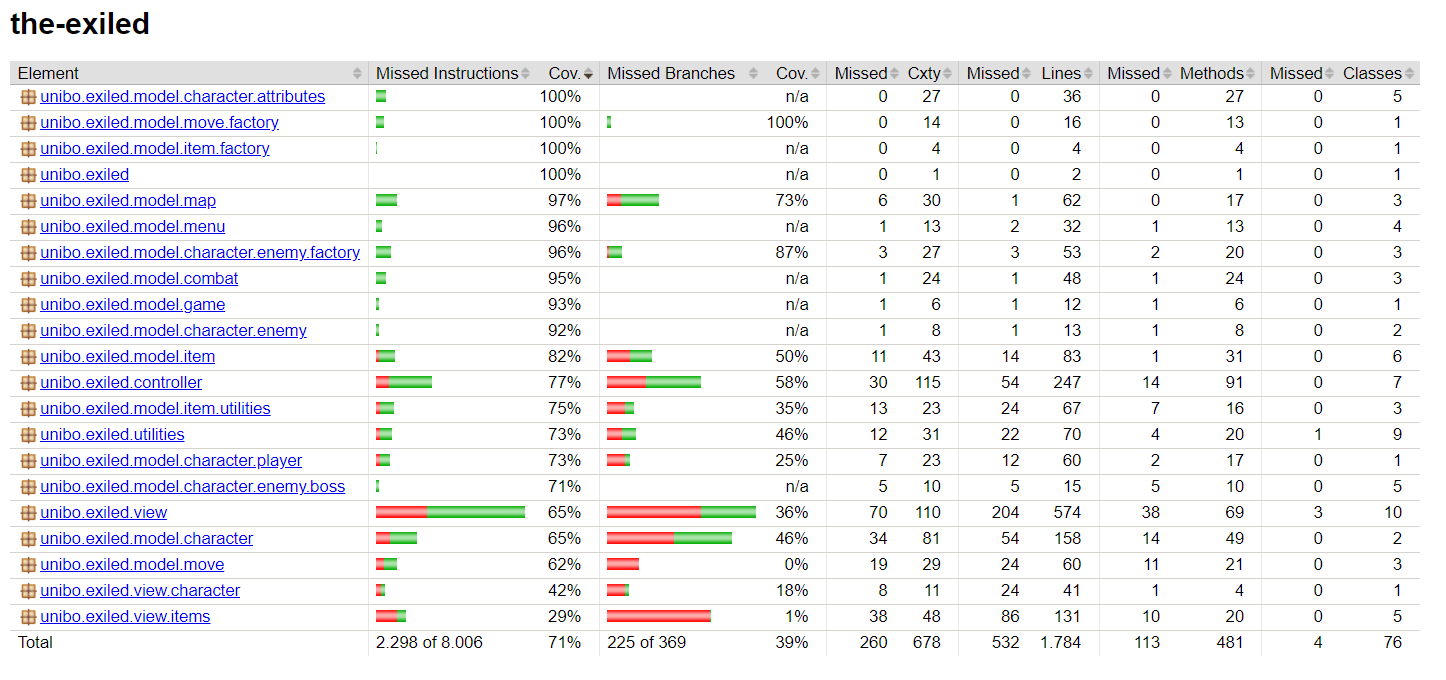
\includegraphics[scale=0.45]{jacoco-report.png}
\end{figure}

\section{Note di sviluppo}

\subsection{Luca Casadei}
Elencherò solamente un'occasione in cui si presentano queste parti di codice più avanzato, questo non impedisce che siano state usate anche in altre parti del progetto.
\begin{itemize}
	\item \textbf{Espressioni Lambda} e \textbf{Optional}: Utilizzati nella classe \textit{CharacterModel} nel metodo \textit{isCellEmpty} per verificare se una cella della mappa contiene qualcuno.\\
	\url{https://github.com/luca-casadei/the-exiled/blob/9a97a74beb0dd351cf5b1f72e6dd4cbeed1acc43/src/main/java/unibo/exiled/model/character/CharacterModelImpl.java#L99-L100}
	\item \textbf{Record}: Gli attributi sono gestiti come dei \textit{Java Records}, in particolare \textit{AdditiveAttributeImpl} e \textit{MultiplierAttributeImpl}.\\
	\url{https://github.com/luca-casadei/the-exiled/blob/9a97a74beb0dd351cf5b1f72e6dd4cbeed1acc43/src/main/java/unibo/exiled/model/character/attributes/AdditiveAttributeImpl.java#L8}
	\item \textbf{Libreria Mockito}: Usata per alcuni tests di JUnit, in particolare il test della classe \textit{CharacterControllerImpl}. Il permalink è relativo ad una piccola parte del codice dove viene usata questa libreria.\\
	\url{https://github.com/luca-casadei/the-exiled/blob/506d8a5ed7be7028e52f6b9613cb84fc03198110/src/test/java/unibo/exiled/controller/TestCharacterControllerImpl.java#L49}
	\item \textbf{\textit{AtomicReference}, \textit{Optional} e Stream}: Ho utilizzato \textit{AtomicReference\textlangle MagicMove\textrangle} per poter avere un riferimento modificabile in maniera atomica in un contesto in cui ho usato ifPresent() di optional per poter utilizzare gli stream. In questo caso mi è servito per poter ritornare il valore desiderato al metodo.
	\url{https://github.com/luca-casadei/the-exiled/blob/4213b41b965a44db1f1a6ffffef8d3c11aab9434/src/main/java/unibo/exiled/model/move/Moves.java#L29-L34}
\end{itemize}

\subsection{Francesco Pazzaglia}

\begin{itemize}
	\item \textbf{Espressioni Lambda}: Utilizzate per le \textit{ActionListener} dei JButton in \textit{EndGameView}. \\
	\url{https://github.com/luca-casadei/the-exiled/blob/a59eb1a55ef30e4a8236a7833d634999110a64a6/src/main/java/unibo/exiled/view/EndGameView.java#L62}
	
	\item \textbf{Optional}: Utilizzati nel \textit{Player}(metodo \textit{getNewMove()}) per la generazione di una nuova mossa. \\
	\url{https://github.com/luca-casadei/the-exiled/blob/b5d735949ba7e010ffae414b746d4d7f464148ba/src/main/java/unibo/exiled/model/character/player/PlayerImpl.java#L127}
	
	\item \textbf{Stream}: Utilizzati nei Controller per controllare che il \textit{Player} abbia vinto il gioco. \\
	\url{https://github.com/luca-casadei/the-exiled/blob/b5d735949ba7e010ffae414b746d4d7f464148ba/src/main/java/unibo/exiled/controller/CharacterControllerImpl.java#L197}
	
	\item \textbf{Font}: Utilizzato nella classe \textit{FontManager} per poter cambiare il font-style del gioco inserendo un font personalizzato. \\
	\url{https://github.com/luca-casadei/OOP23-the-exiled/blob/884364614a6dbfb22a62d7c36e7baecd75401f6a/src/main/java/unibo/exiled/utilities/FontManager.java#L12} \\
	Ho preso spunto dalla documentazione Oracle: \\ \url{https://docs.oracle.com/javase/tutorial/2d/text/fonts.html}.
\end{itemize}

\subsection{Marco Magnani}
\begin{itemize}
	\item \textbf{Stream e Optional}: Utilizzati sia nell' \textit{ItemContainer} che nelle \textit{Moves} per ricavare esempio un item in base al tipo.\\ \url{https://github.com/luca-casadei/the-exiled/blob/71356cacbbef08c33f96d68802a33514823d3571/src/main/java/unibo/exiled/model/item/utilities/ItemsContainer.java#L76C7-L76C8}
	\item \textbf{Stream}: In \textit{CharacterModelImpl} utilizzato per evitare la compenetrazione di enemy all'interno della mappa, aggiunto nel commit con hash: f25b577fb319fbbcb38154b3f2b8a3233d5c561b\\
	\url{https://github.com/luca-casadei/the-exiled/blob/71356cacbbef08c33f96d68802a33514823d3571/src/main/java/unibo/exiled/model/character/CharacterModelImpl.java#L159C1-L160C1} 
	\item \textbf{Optional}: In \textit{ElementalType} e \textit{ItemNames} il metodo per prendere le relative immagini ritorna un Optional per gestire il caso in cui la mossa non sia presente nel progetto\\
	\url{https://github.com/luca-casadei/the-exiled/blob/71356cacbbef08c33f96d68802a33514823d3571/src/main/java/unibo/exiled/model/item/utilities/ItemNames.java#L83C1-L84C55}
	\item \textbf{Stream}: Nella \textit{ItemsModel} utilizzata per la conversione da \textit{Map\textless Item,Integer\textgreater} a \textit{Map\textless String,Integer\textgreater} ed anche per filtrare gli oggetti in base al nome, aggiunto nel GameModel commit con hash: 2e72b6911f473bfa3ee8685cd61f14ae8922f936\\
	\url{https://github.com/luca-casadei/the-exiled/blob/71356cacbbef08c33f96d68802a33514823d3571/src/main/java/unibo/exiled/model/item/ItemsModelImpl.java#L28C1-L28C90}
	\item \textbf{Stream}: In \textit{InventoryView} quando vengono aggiornati i bottoni contenenti gli item li ordino in modo da migliorarne la visualizzazione.
	\url{https://github.com/luca-casadei/the-exiled/blob/b0f1e9a189dbf365a0413e7249402b7342fd88a7/src/main/java/unibo/exiled/view/InventoryView.java#L106C1-L108C47}
\end{itemize}


\subsection{Manuel Baldoni}
\begin{itemize}
	\item \textbf{Stream}: Utilizzato nel metodo \textit{getEnemyRandomMoveName}. Per avere il nome di una mossa randomica.\\ \url{https://github.com/luca-casadei/OOP23-the-exiled/blob/2607859d3adef7b5c23090199e0807cd852fc256/src/main/java/unibo/exiled/controller/CombatControllerImpl.java#L137C5-L148C6}
	\item \textbf{Stream}: Utilizzato nel metodo \textit{attack}. Per trovare la mossa effettuata dall'attaccante dal suo moveset.\\ \url{https://github.com/luca-casadei/OOP23-the-exiled/blob/2607859d3adef7b5c23090199e0807cd852fc256/src/main/java/unibo/exiled/controller/CombatControllerImpl.java#L156C2-L259C6}
	\item \textbf{Optional ed Espressioni Lambda}: Utilizzate per le verificare la presenza dell'item droppato dal nemico e per aggiungerlo all'inventario.
	\url{https://github.com/luca-casadei/OOP23-the-exiled/blob/2607859d3adef7b5c23090199e0807cd852fc256/src/main/java/unibo/exiled/controller/CombatControllerImpl.java#L203C9-L214C10}
	\item \textbf{Espressione Lambda}: Utilizzata per gestire il listener del comando del menu.
	\url{https://github.com/luca-casadei/OOP23-the-exiled/blob/2607859d3adef7b5c23090199e0807cd852fc256/src/main/java/unibo/exiled/view/MenuView.java#L67C9-L91C12}
	\url{https://github.com/luca-casadei/OOP23-the-exiled/blob/2607859d3adef7b5c23090199e0807cd852fc256/src/main/java/unibo/exiled/view/CombatView.java#L95C17-L99C20}
\end{itemize}

\subsection{Codice preso da esterni}
\begin{itemize}
	\item \textbf{Wrap Layout}: E' un componente che estende il FlowLayout di \textit{java.awt}, consente ai componenti del Layout stesso di "andare a capo" quando occupano troppo spazio rispetto alla dimensione(altezza e larghezza) della finestra.\\ 
	\url{https://gist.github.com/jirkapenzes/4560255}
\end{itemize}

\chapter{Commenti finali}

\section{Autovalutazione e lavori futuri}

\subsection{Luca Casadei}
Personalmente ritengo che il mio contributo all'interno del team di sviluppo sia stato importante, sia per la parte realizzativa che per quella decisionale, ma non più importante di quella degli altri componenti del gruppo, con i quali è stato possibile lo confrontare le proprie idee di realizzazione, la corretta suddivisione dei compiti e uno sviluppo continuativo dell'applicazione anche se non necessariamente tutti presenti allo stesso momento o nello stesso luogo. Anche il caricamento del codice in parallelo con sistemi di controllo della versione è avvenuto in maniera secondo me pulita, perché tutti sono stati in grado di adottare questi strumenti in modo efficace senza creare troppi intoppi. Siccome la progettazione finale del progetto secondo me risulta abbastanza scalabile, non è esclusa l'ipotesi di arricchire ulteriormente il contenuto del gioco e le sue componenti, anche prendendo in forte considerazione la valutazione dei docenti.

\subsection{Francesco Pazzaglia}

Nonostante le parti complesse del progetto e il fatto di sviluppare un progetto in team mi avesse inizialmente intimorito, sono soddisfatto di come siamo riusciti a completare e consegnare il gioco. Di solito sono abituato a lavorare da solo, ma ho trovato la collaborazione del team piuttosto soddisfacente. Lo scambio di idee e il confronto ci hanno aiutato a coordinarci efficacemente, individuando i metodi e le classi necessarie per varie parti del progetto. Lavorare in team è stato molto formativo e mi ha permesso di apprezzare come si possa realizzare un progetto insieme, nonostante stili di programmazione talvolta diversi.

\subsection{Marco Magnani}
Il progetto è stato svolto con colleghi con cui ho avuto modo di collaborare già in precedenza alle superiori, quindi sapevo già prima cosa aspettarmi. La centralità della collaborazione e della discussione di idee è stata una costante durante lo sviluppo di questo progetto. Nel complesso, ritengo che il nostro lavoro sia stato soddisfacente, e in particolare, credo di aver gestito una buona parte del progetto sfruttando le competenze acquisite durante le lezioni.

\subsection{Manuel Baldoni}
Credo che tutti i componenti del gruppo siano individualmente molto preparati a livello di competenze di sviluppo e credo che siamo riusciti a collaborare in maniera efficace. Personalmente credo di aver svolto la mia parte di progetto in maniera efficace ed efficiente. Il mio contributo nelle altri parti del progetto sicuramente non è stato nel volume degli altri componenti del gruppo, tuttavia penso che alcuni miei interventi siano stati fondamentali per la realizzazione del progetto.

\section{Difficoltà incontrate e commenti per i docenti}
Nessun commento o difficoltà da segnalare.

\appendix
\chapter{Guida utente}
Per la maggior parte delle azioni compibili nel gioco sono presenti bottoni sull'interfaccia, non è quindi necessario conoscere nessun particolare comando. Ne sono stati aggiunti alcuni aggiuntivi nell'inventario per l'apertura e la chiusura, come sottodescritto.
\section{Movimento}
Per muoversi sulla mappa a celle si usano i comandi:
\begin{itemize}
	\item \textit{W} per andare su.
	\item \textit{S} per andare giù.
	\item \textit{A} per andare a sinistra.
	\item \textit{D} per andare a destra.
\end{itemize}
\section{Inventario}
Si può aprire l'inventario con \textit{E} e richiuderlo con \textit{ESC}
\section{Menu}
Si può aprire il menu di gioco utilizzando \textit{ESC} quando si visualizza la mappa, e richiuderlo in maniera analoga.

\chapter{Esercitazioni di laboratorio}
Elenco dei Permalink delle consegne nel forum studenti del modulo di laboratorio.
\section*{Consegne}
\subsection{luca.casadei27@studio.unibo.it}
\begin{itemize}
	\item Laboratorio 06: \url{https://virtuale.unibo.it/mod/forum/discuss.php?d=146511#p208401}
	\item Laboratorio 07: \url{https://virtuale.unibo.it/mod/forum/discuss.php?d=147598#p209323}
	\item Laboratorio 08: \url{https://virtuale.unibo.it/mod/forum/discuss.php?d=148025#p209782}
	\item Laboratorio 09: \url{https://virtuale.unibo.it/mod/forum/discuss.php?d=149231#p211336}
	\item Laboratorio 10: \url{https://virtuale.unibo.it/mod/forum/discuss.php?d=150252#p212475}
\end{itemize}

\end{document}